% Unlike a LaTeX article or report, this slide presentation is done with the beamer class
\documentclass{beamer}
%\usepackage{etex}
% This information is compiled into the title page
\title{Master's Project Defense}
\subtitle{Infinite Levels of Complexity in a Family\\ of One-Dimensional Singular Dynamical Systems}
\author{Evan Oman}
\institute{\normalsize University of Minnesota Duluth}
\date{May 14, 2015}


% The following package allows for different themes.
\usepackage{beamerthemesplit,fancyvrb}
\usetheme{Copenhagen} %Antibes Bergen Berkeley Berlin Boadilla Copenhagen Darmstadt DresdenFrankfurt Goettingen Hannover IlmenauJuanlespins Madrid Malmoe MarburgMontpellier Paloalto Pittsburgh Singapore

% These packages allow use of some of the more common math commands
\usepackage{amsmath,amssymb, wrapfig, float, subcaption, caption,multicol}

\usepackage{graphicx}
% \usepackage{html}

\usepackage{float}
%\usepackage{graphicx}
\useoutertheme{sidebar}
%\patchcmd{\chapter}{\if@openright\cleardoublepage\else\clearpage\fi}{}{}{}
%\makeatother

\floatstyle{plaintop}

\DeclareGraphicsRule{.JPG}{eps}{*}{`jpeg2ps #1}


\newtheorem{innercustomthm}{\bf Proposition}
\newenvironment{customthm}[1]
{\renewcommand\theinnercustomthm{#1}\innercustomthm\itshape}
{\endinnercustomthm}
\usepackage{color}
% \setbeamercolor*{palette tertiary}{bg=Brown}
\setbeamercolor{frametitle}{fg=white}%},bg=Brown!20}

\renewcommand*{\thefootnote}{\fnsymbol{dagger}}

\newtheorem{proposition}{\bf Proposition}


%Some nice commands from my header file:
\newcommand{\ds}{\displaystyle}
\newcommand{\R}{\mathbb{R}}
\newcommand{\Q}{\mathbb{Q}}
\newcommand{\Z}{\mathbb{Z}}
\newcommand{\C}{\mathbb{C}}
\newcommand{\N}{\mathbb{N}}
\newcommand{\<}{\left\langle}
\renewcommand{\>}{\right\rangle} %Better check at some point to make sure \> isn't anything important
\renewcommand{\*}{\cdot} %Better check at some point to make sure \* isn't anything important
\newcommand{\inv}{^{-1}}
\newcommand{\sol}[1]{\begin{solution}#1\end{solution}}
\newcommand{\al}[1]{\begin{align*}#1\end{align*}}
\newcommand{\ov}[1]{\overline{#1}}

\newcommand{\ra}{\rightarrow}
\newcommand{\Ra}{\Rightarrow}

\newcommand{\pl}{p^{-C}_1}
\newcommand{\pr}{h^{CrP_c}_2}
\newcommand{\inte}[2]{\text{int}\{#1,#2\}}



%CHANGE TO ADD INDENTATION
\setlength{\parindent}{0in}
\mode <presentation>

\begin{document}


\maketitle

\tableofcontents

\section{Introduction}
\begin{frame}
	\frametitle{Introduction}
	\begin{itemize}
		\item The goal of Dynamical Systems is to develop a characterization of the behavior of all points under some map of interest
		\item A great amount of effort has been dedicated to studying rational maps of the plane such that $f: \R^2 \ra \R^2$
		\item One well known rational map is the quadratic map 
		\[z_n \mapsto Q_c (z_n) = z_n^2 + c = z_{n+1}\]
		\item In this talk we will discuss the perturbed system 
		\[z_n \mapsto f_{c, \beta} (z_n) = z_n^2 + c + \frac{\beta}{\overline{z_n}^2} = z_{n+1}\]
	\end{itemize}
\end{frame}

\section{Background}
\subsection{Definitions}
\begin{frame}
	\frametitle{Orbits and Long Term Behavior}
	\begin{itemize}
		\item Suppose we want to describe the dynamics of some map $f_{\alpha_1,\alpha_2, \cdots, \alpha_n} : S\ra S$ ($\R$ or $\R^2$)
		\item More specifically, our goal is to characterize the long term behavior of the orbit of every point in the domain as the set of parameters vary
	\end{itemize}

	\begin{definition}{Forward Orbit of a Discrete System\cite{Dev2}:}
		The forward orbit of some $x \in S$ is the set of points $x, f (x), f^2 (x),\ldots$ and is denoted by $O^+ (x)$.
	\end{definition}

	\begin{itemize}
		\item Thus we will attempt to determine some way of describing the limiting behavior of all points in the domain
	\end{itemize}
\end{frame}

\begin{frame}
	\frametitle{Boundedness}
	\begin{itemize}
		\item Generally this is impossible so we start with a more general dichotomy: bounded vs. unbounded
		\item Unbounded orbits grow arbitrarily large and limit to $\infty$
		\item Bounded orbits remain within some ball of finite radius
		\item There are many ways that a point may stay bounded
	\end{itemize}
\end{frame}

\begin{frame}
	\frametitle{Fixed and Periodic Points}
	\begin{definition}{Fixed and Periodic Orbits\cite{Dev2}:}
		The point $x$ is a fixed point for $f$ if $f (x) = x$. The point $x$ is a periodic point of period $n$ if $f^n (x) = x$. The least positive $n$ such that $f^n (x) = x$ is called the prime period of $x$. The set of points in the orbit of a periodic point form a periodic orbit. 
	\end{definition}

	\begin{definition}{Attracting and Repelling Fixed Points\cite{Dev1}:}
		Suppose $x_0$ is a fixed point for $f$ where $f$ is a one dimensional map. Then $x_0$ is an attracting fixed point if $|f' (x_0) | < 1$. The point $x_0$ is a repelling fixed point if $|f' (x_0)| > 1$. Finally, if $|f' (x_0)| = 1$, the fixed point is called (linearly)neutral or indifferent.
	\end{definition}
\end{frame}

\begin{frame}
	\frametitle{Critical Points}
	\begin{itemize}
		\item Points may also be eventually fixed/periodic or in some cases remain bounded while densely filling an interval (such as in the case of a chaotic system)
		\item Another way to simplify the problem is to look at points affect the behavior of the entire system, such as critical points
	\end{itemize}
	\begin{definition}{Critical Point \cite{Dev2}:}
		A point $x$ is a critical point of a one dimensional map $f$ if $f' (x) =0$. The critical point is degenerate if $f'' (x)  = 0$ or non-degenerate otherwise.
	\end{definition}
	% \begin{itemize}

	% \end{itemize}
\end{frame}
\subsection{Visualization Methods}
\begin{frame}
	\frametitle{Visualization Techniques}
	\begin{itemize}
		\item Graphical Iteration: A method of displaying a small number of iterates for a one dimensional system in $ (x_n, x_{n+1})$ space
		\item Orbit Diagram: A method of showing approximate long term behavior over a range of parameter values by plotting hundreds of points. Orbit Diagrams exist in parameter $\times$ phase space.
		\item Escape Diagrams: A method for two dimensional systems where we have a plane of initial conditions (each represented by a pixel) such that each pixel is then colored by the relative escape ``time'' of that initial condition. Escape pictures can exist in phase space ($x = (x_1, x_2)$) or parameter space ($c = (c_1, c_2)$)
	\end{itemize}
\end{frame}

\begin{frame}
	\frametitle{Graphical Iteration}
	\begin{figure}
		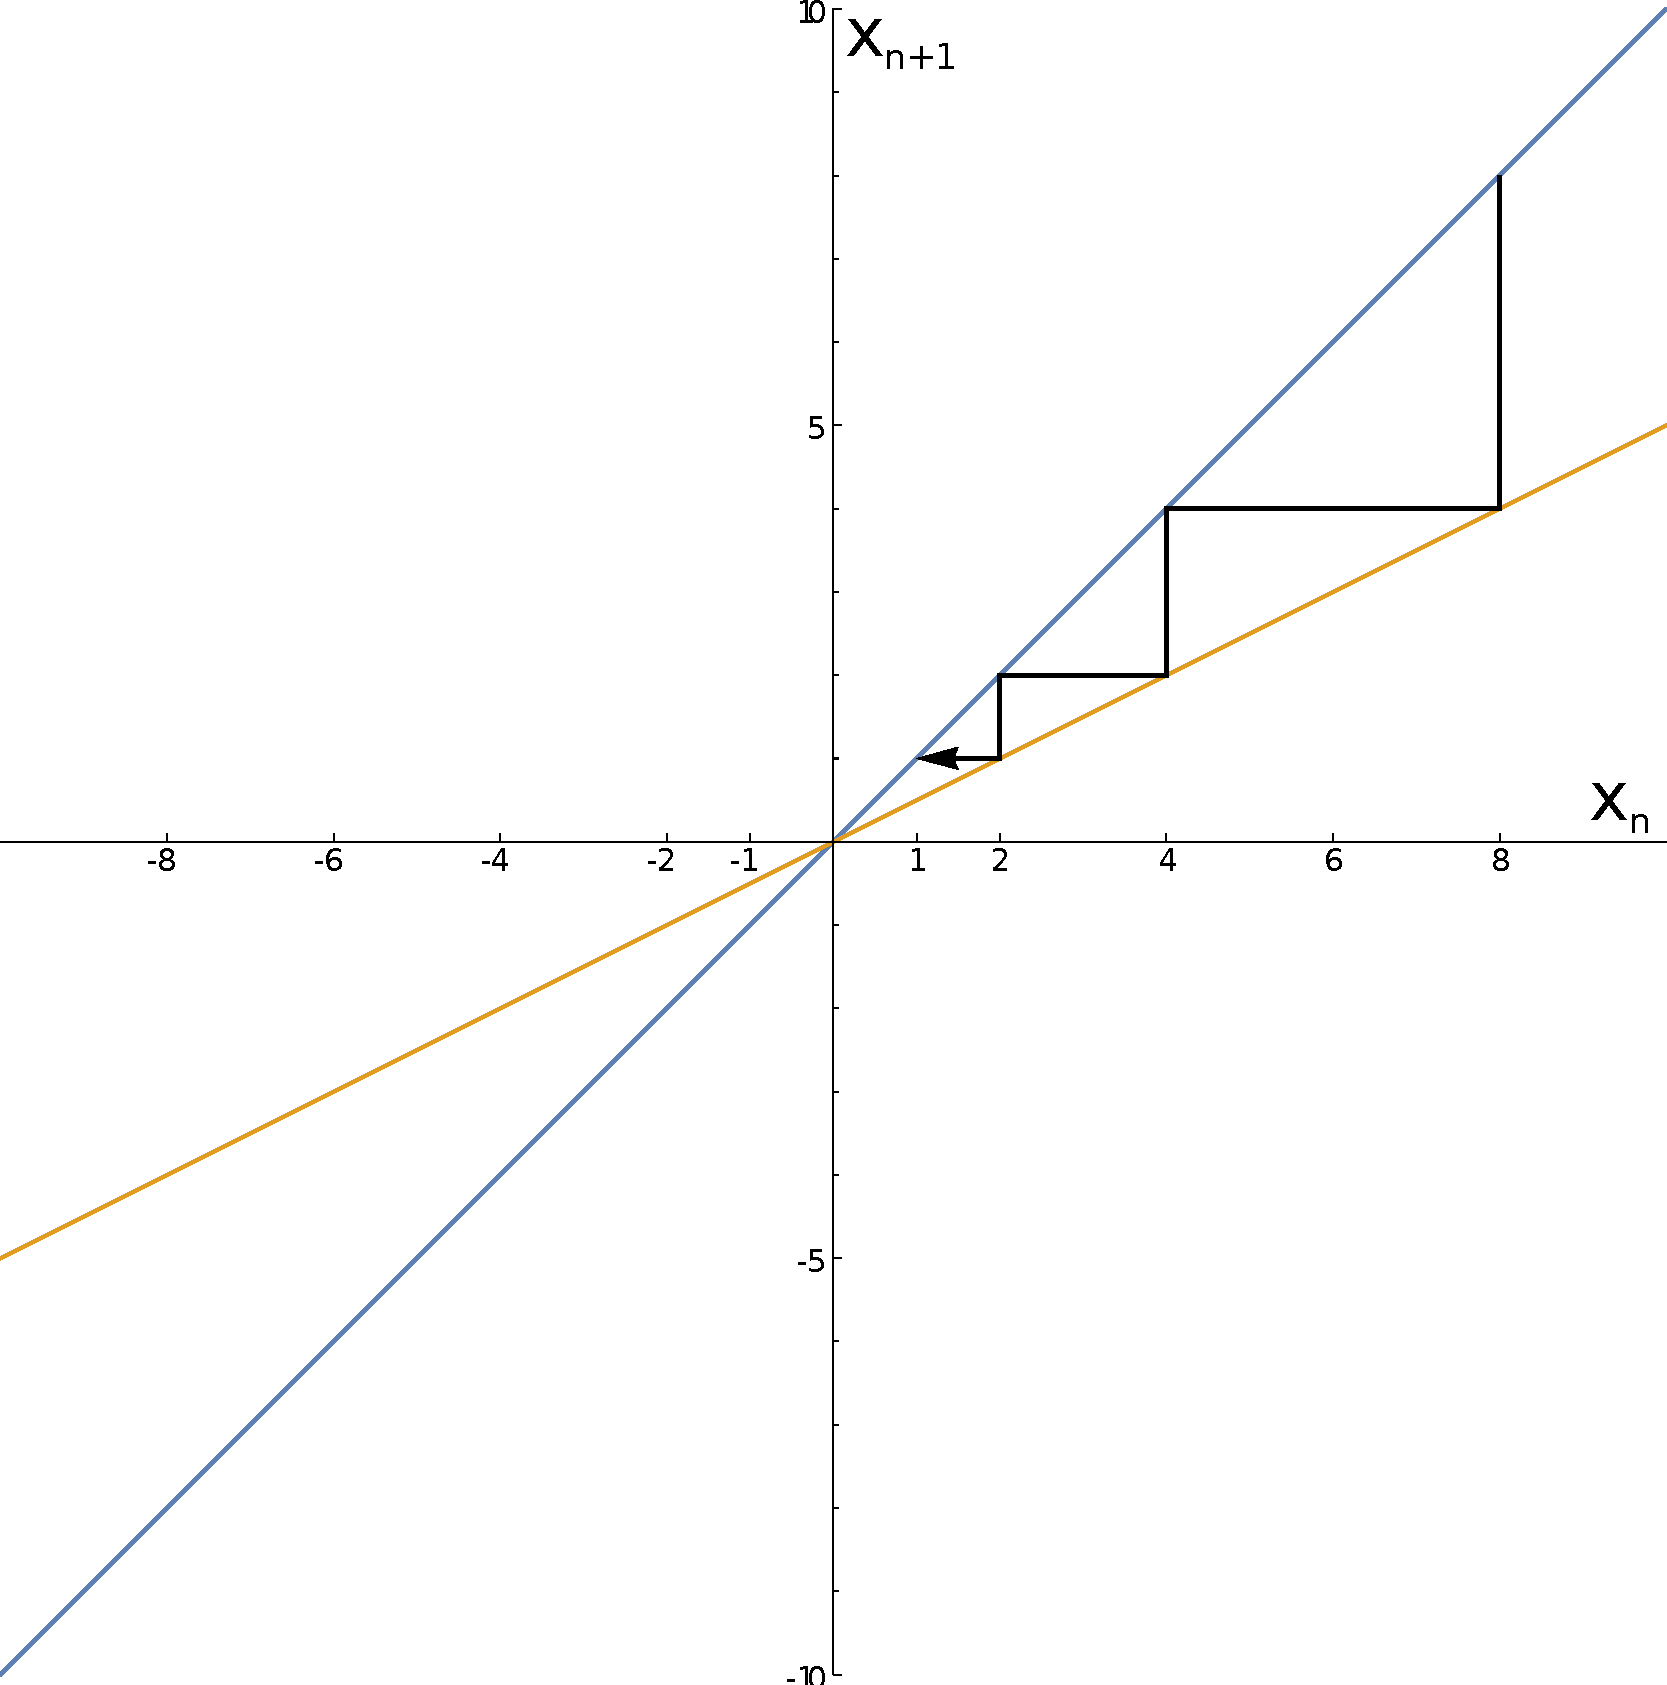
\includegraphics[height=.85\textheight]{./img/simplegraphit}
		\caption{Graphical iteration of $x_0 = 8$ on $x_{n+1} = \frac{1}{2}x_n$}
	\end{figure}
\end{frame}

\begin{frame}
	\frametitle{Orbit Diagram}
	\begin{figure}
		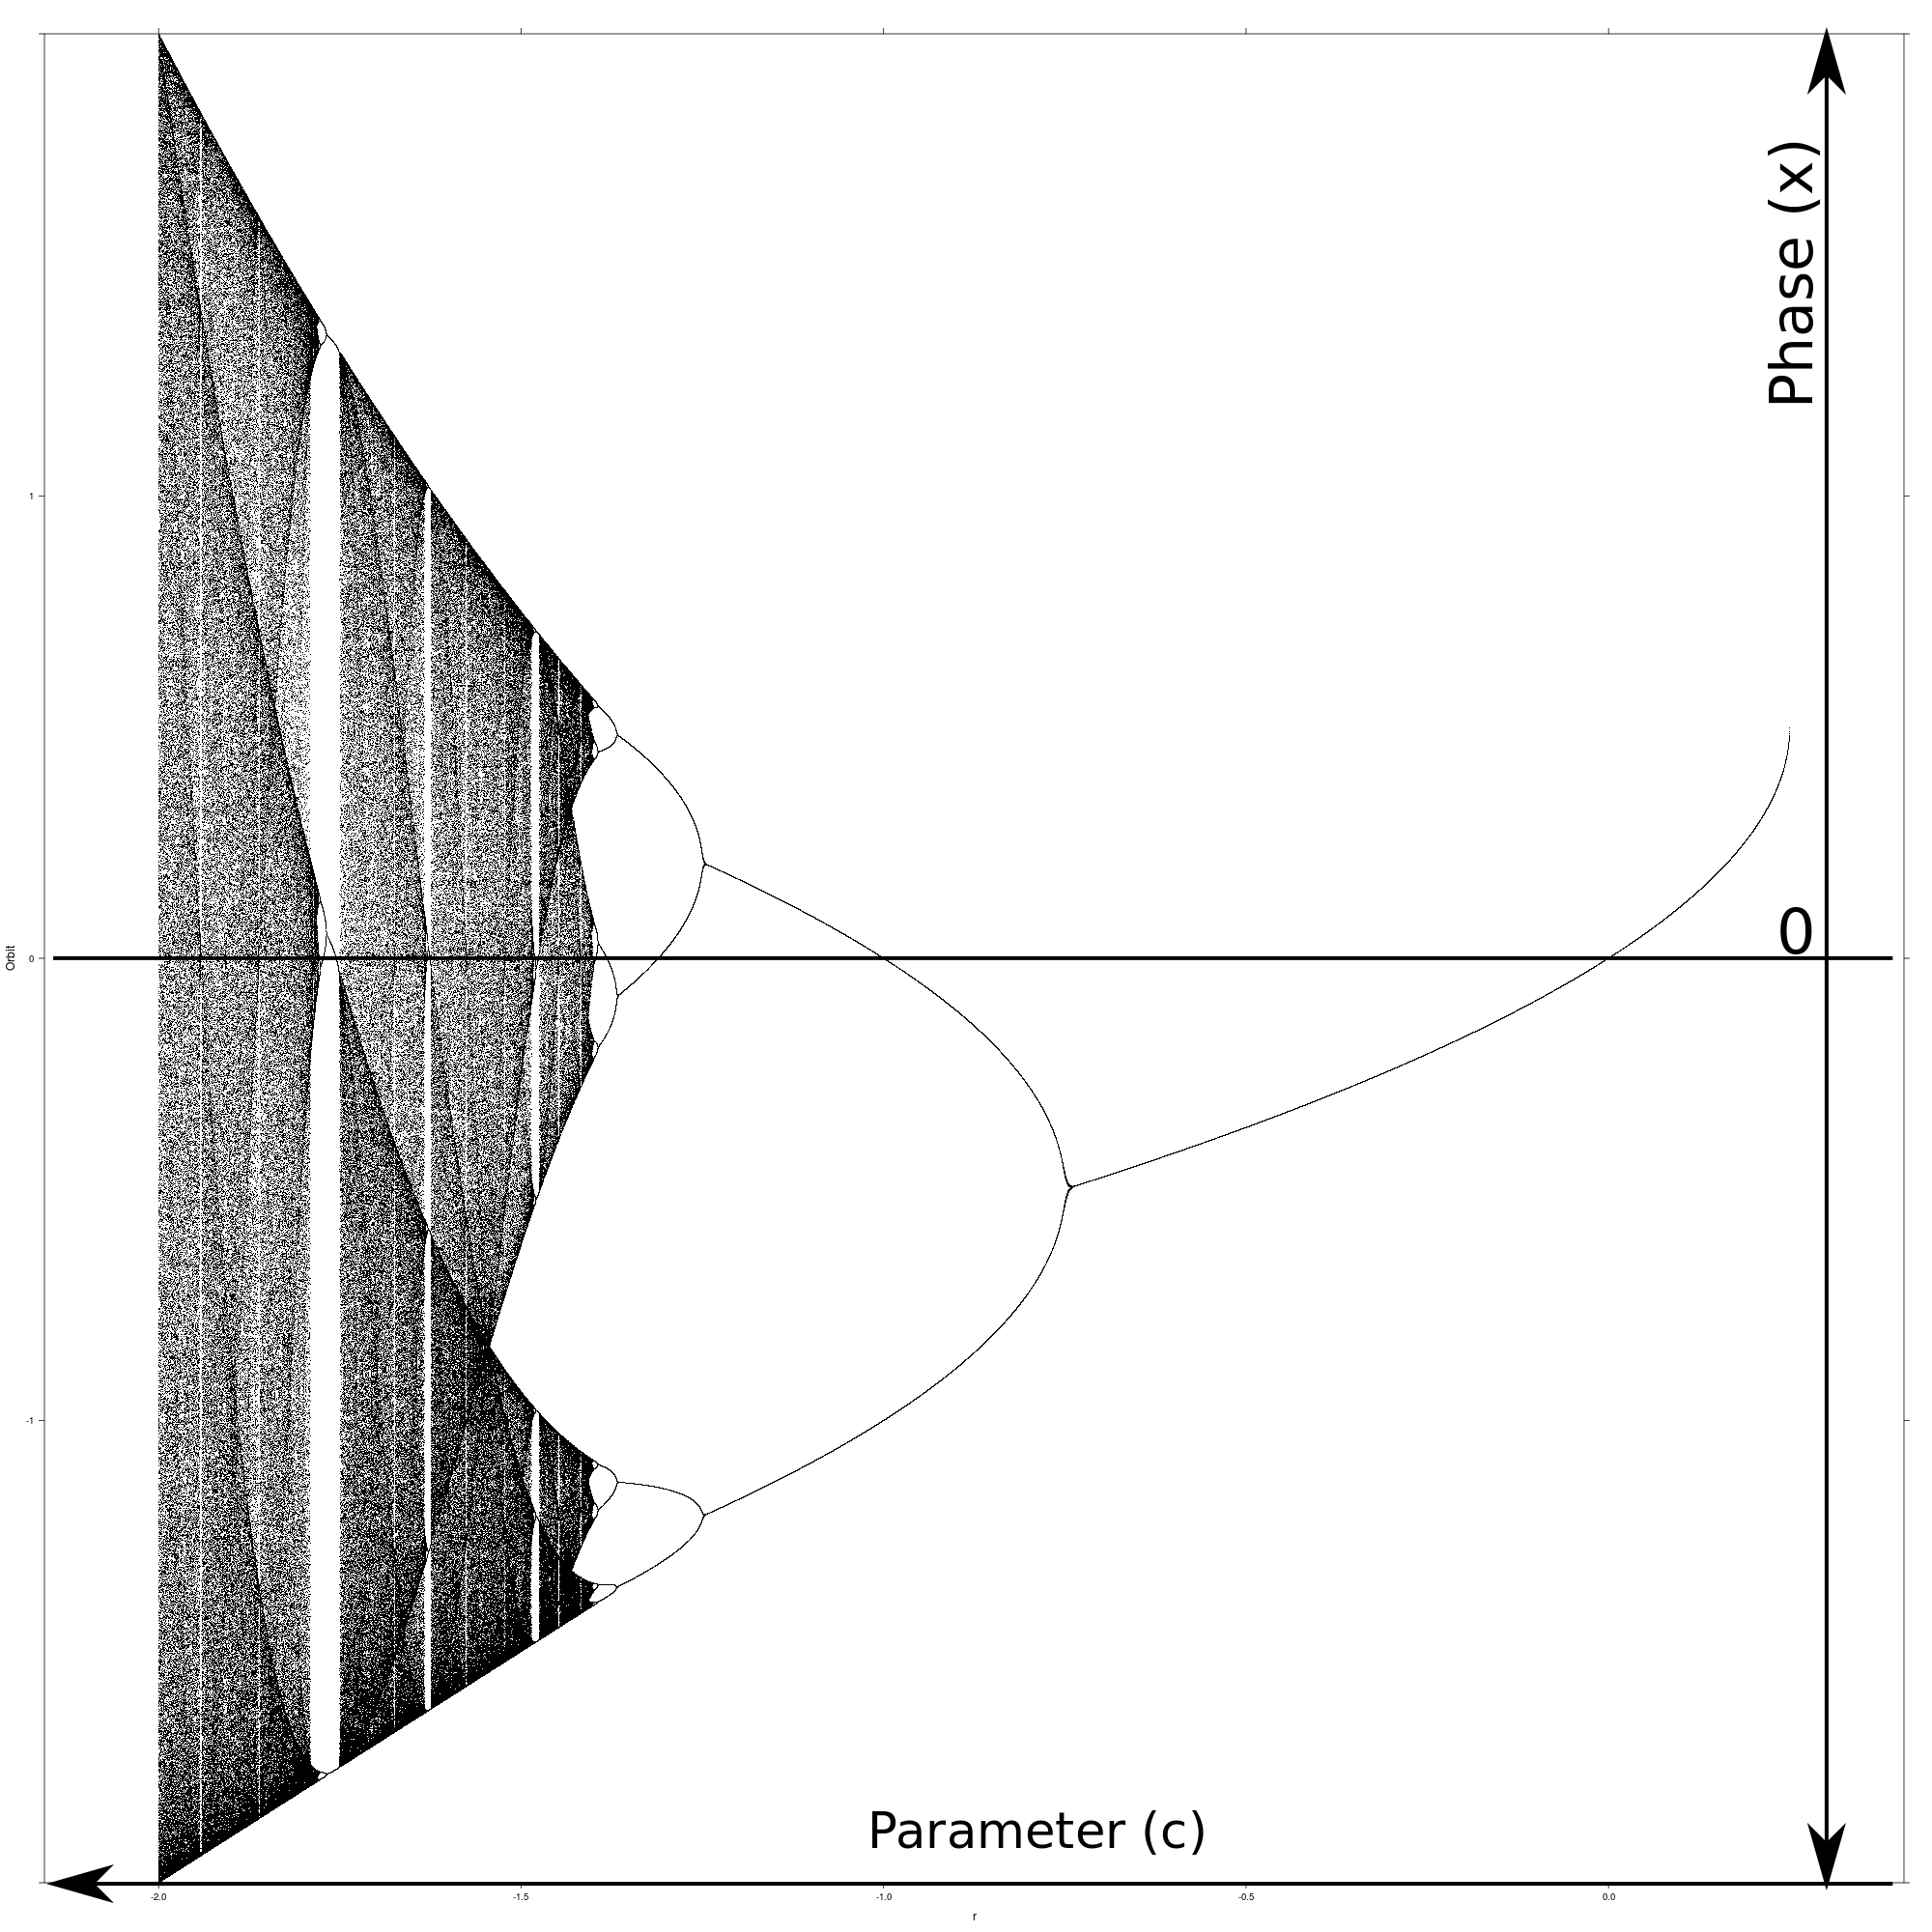
\includegraphics[height=.85\textheight]{./img/original.png}
		\caption{Orbit Diagram for $Q_c (x) = x^2 + c$}
	\end{figure}
\end{frame}

\begin{frame}
	\frametitle{Orbit Diagram + Graphical Iteration}
	\begin{figure}
		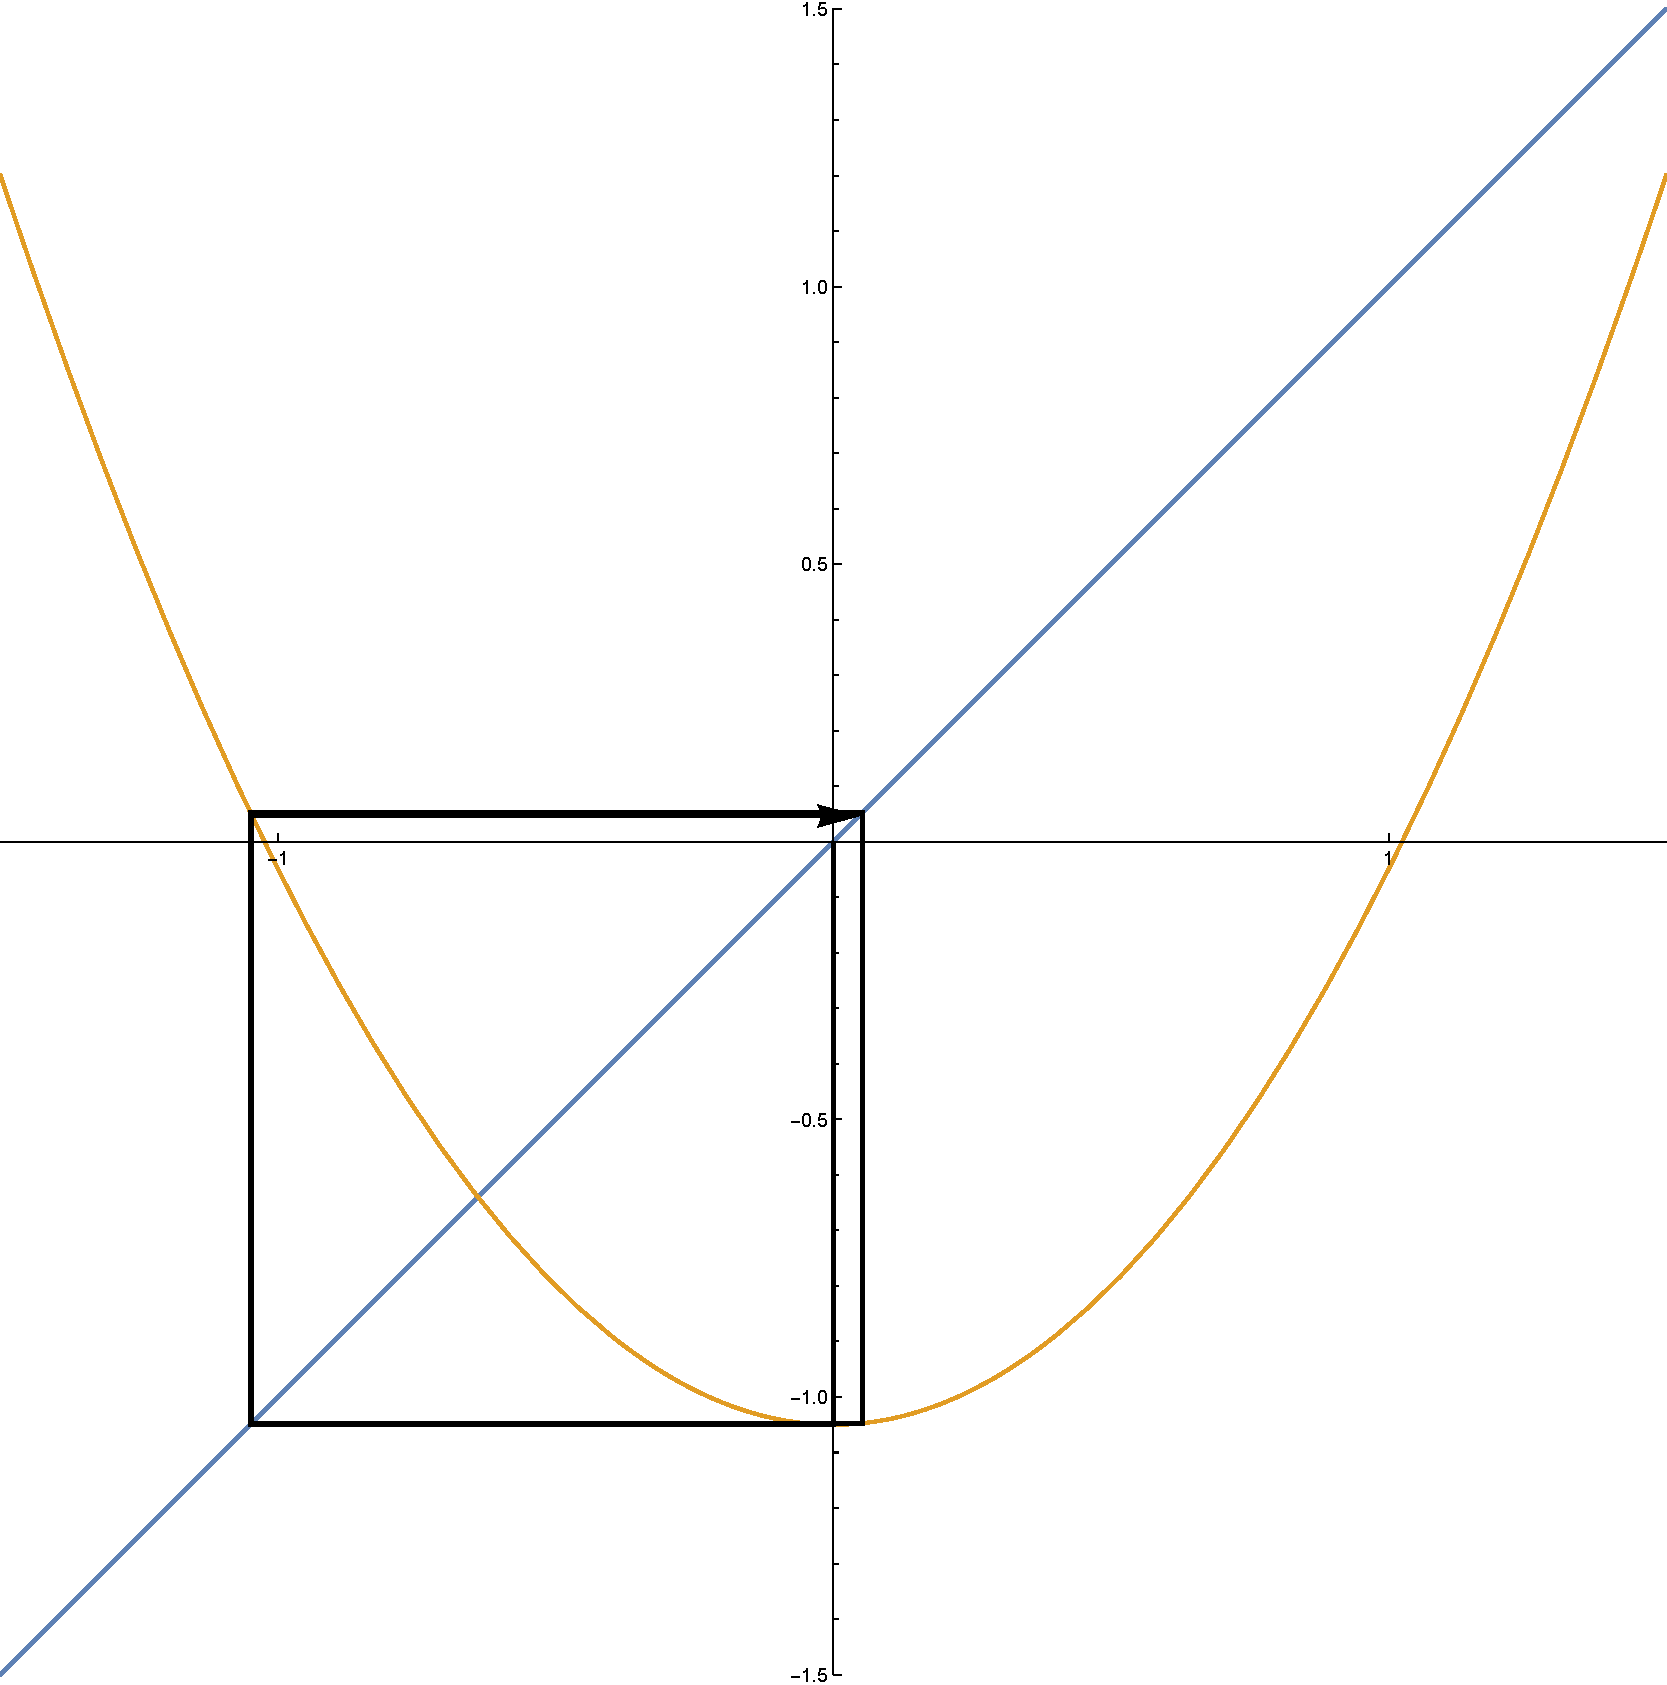
\includegraphics[height=.85\textheight]{./img/plot3_-105}
		\caption{Graphical iteration of the critical point on $x_{n+1} = x_{n}^2 - 1.05$}
	\end{figure}
\end{frame}

\begin{frame}
	\frametitle{Escape Picture}
	\begin{figure}
		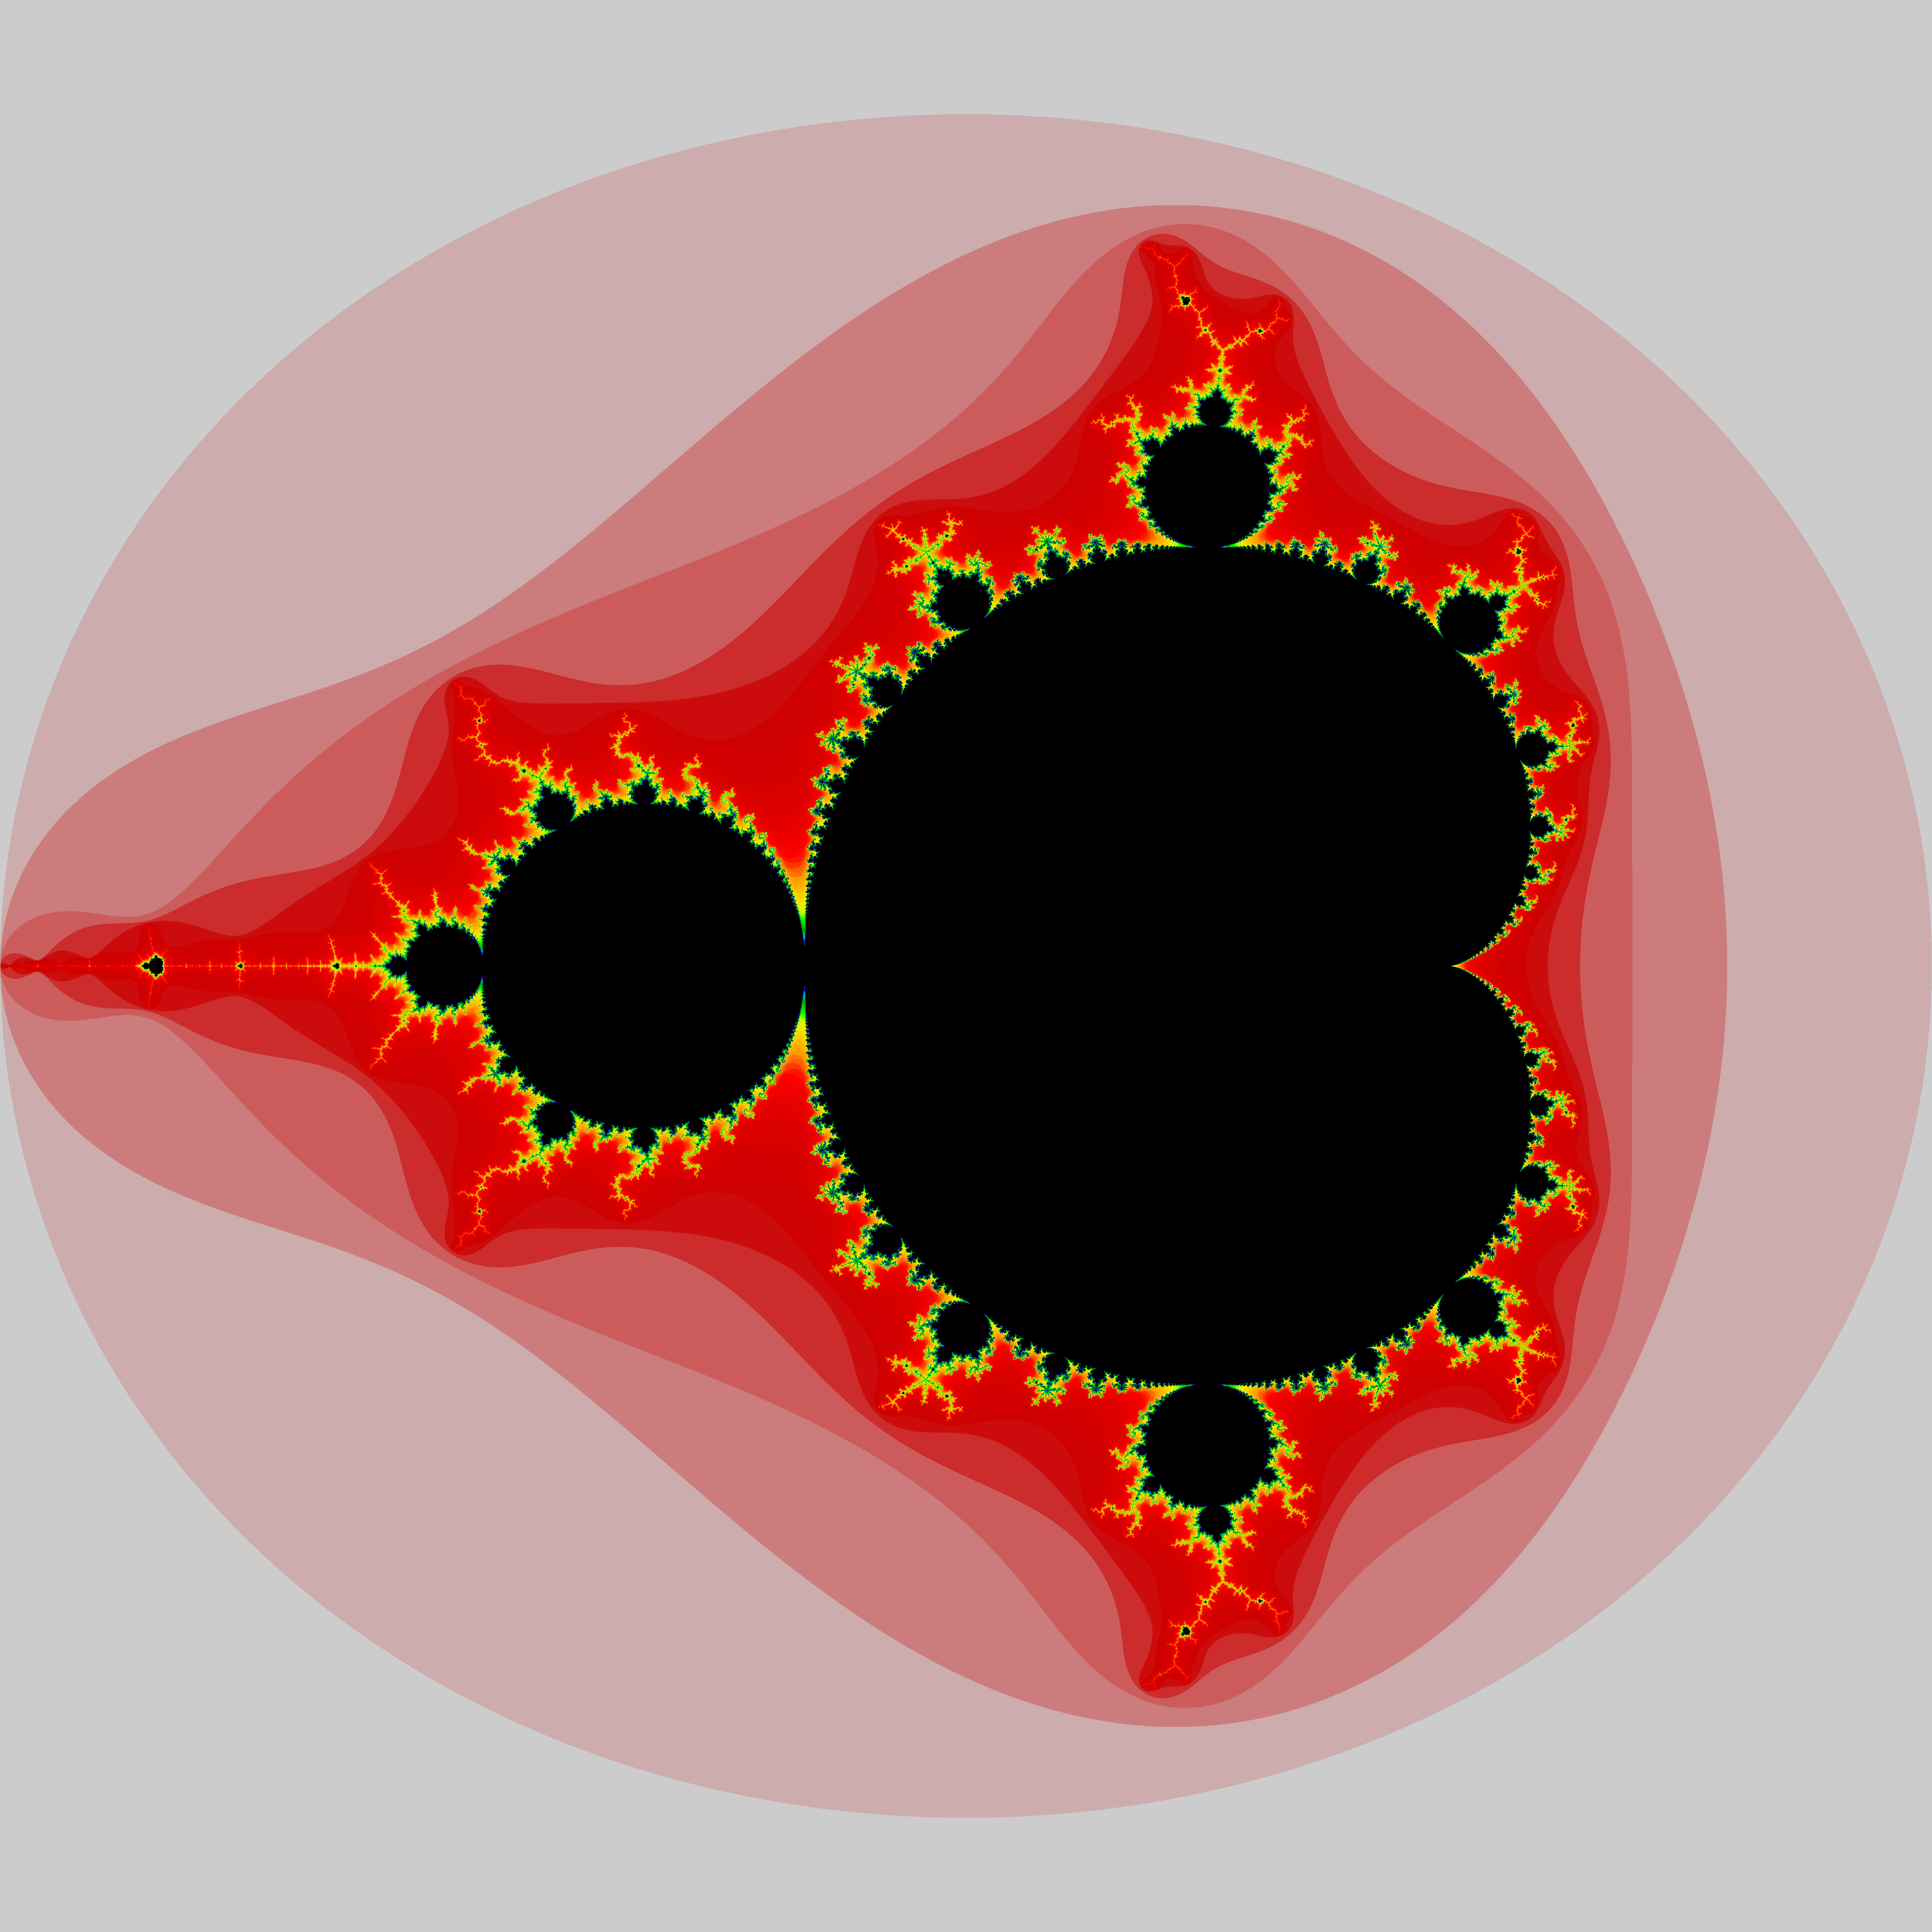
\includegraphics[height=.75\textheight]{./img/b000.png}
		\caption{Parameter Escape Picture for $Q_c (z) = z^2 + c$}
	\end{figure}
\end{frame}
\section{Results}
\subsection{Numerical Experimentation}
\begin{frame}
	\frametitle{Perturbed Map}
	\begin{itemize}
		\item We can now move on to a discussion our system:
	\end{itemize}
		{\small\[
			f_{c, \beta} (x) = z^2 + c + \frac{\beta}{\overline{z}^2} \text{ for } z,c, \beta \in \C 
		\]
		\[
			f_{c, \beta} (x) = x^2 + c + \frac{\beta}{x^2} \text{ for } x,c, \beta \in \R 
		\]}
		\begin{figure}
			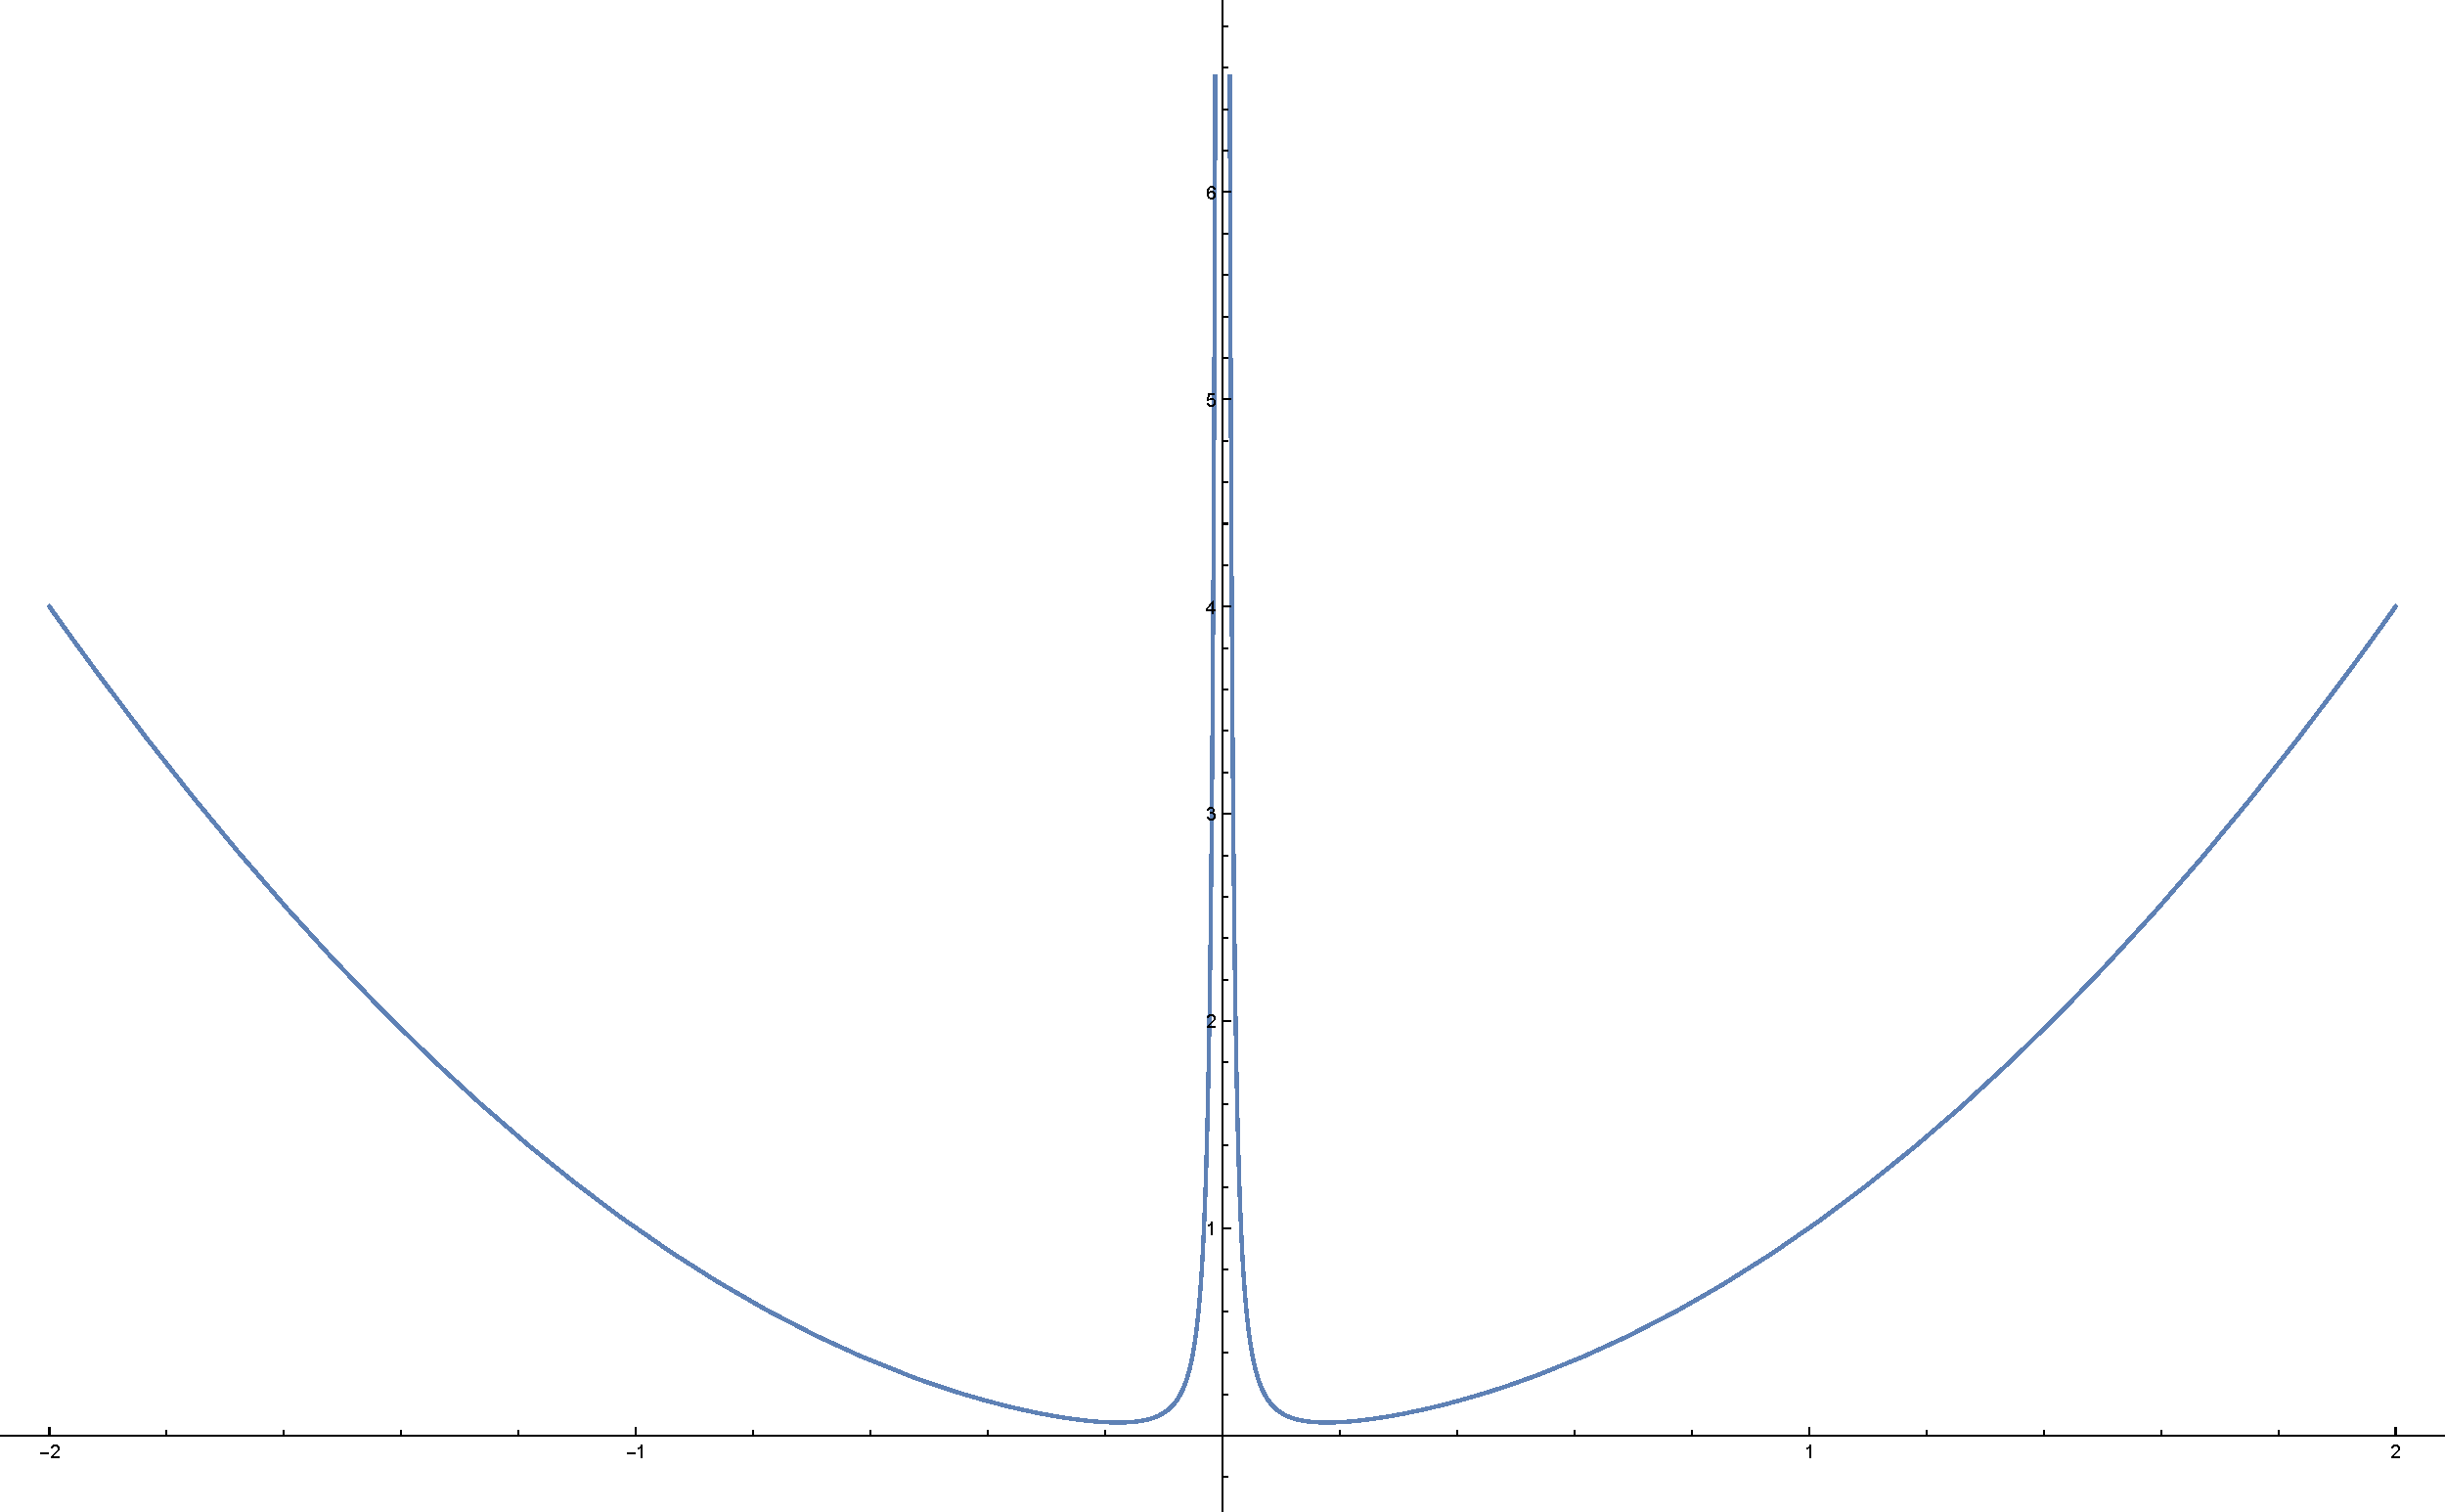
\includegraphics[height = .5\textheight]{./img/singplot}
			\caption{Plot of $f_{0,.001} = x^2 + \frac{.001}{x^2}$}
		\end{figure}
\end{frame}

\begin{frame}
	\frametitle{Comparison of Orbit Diagrams}
	\begin{figure}[h]
		\centering
		\begin{subfigure}[b]{0.5\textwidth}
				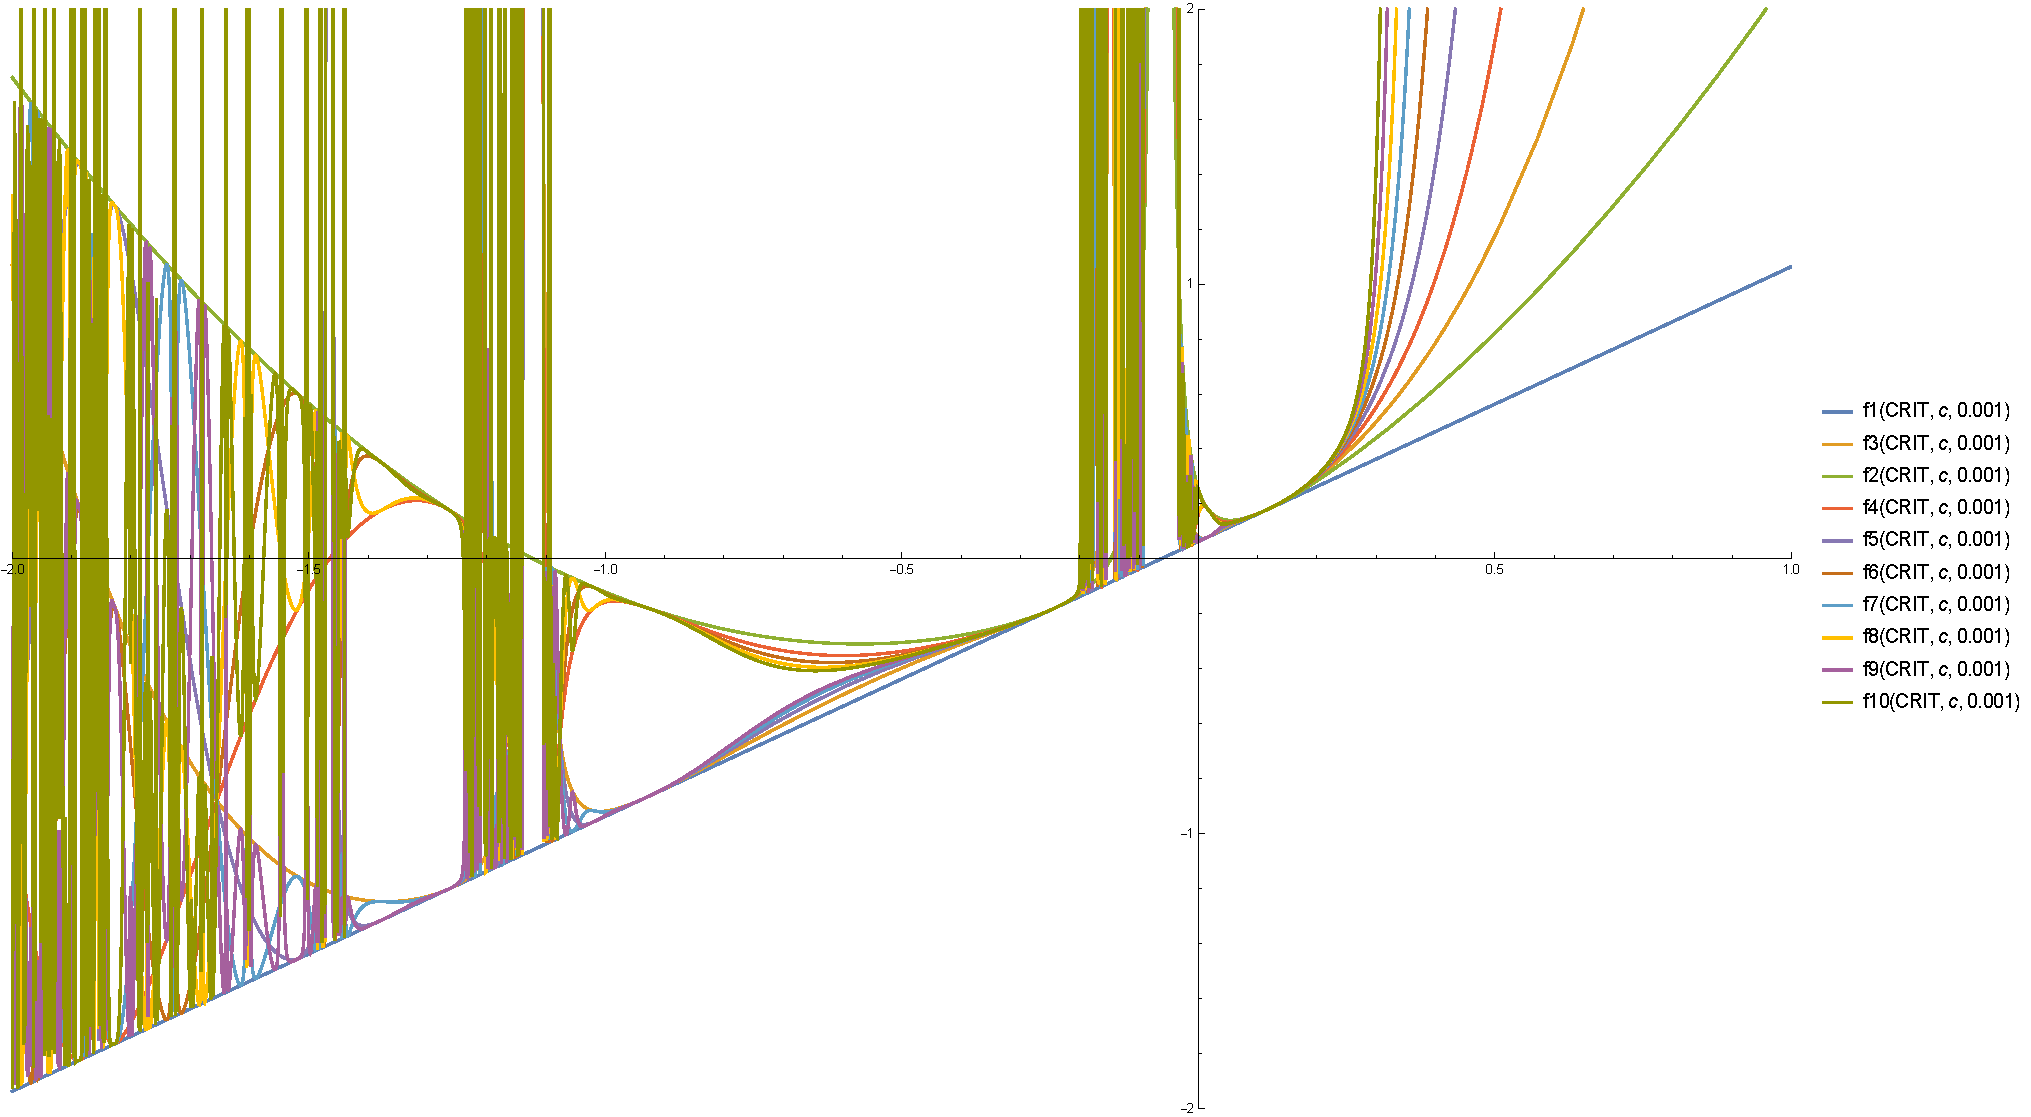
\includegraphics[width=\textwidth]{./img/pert}
				\caption{Orbit diagram of $x^2 + c + \frac{.001}{x^2}$}
				\label{pert}
		\end{subfigure}%
		\begin{subfigure}[b]{0.5\textwidth}
				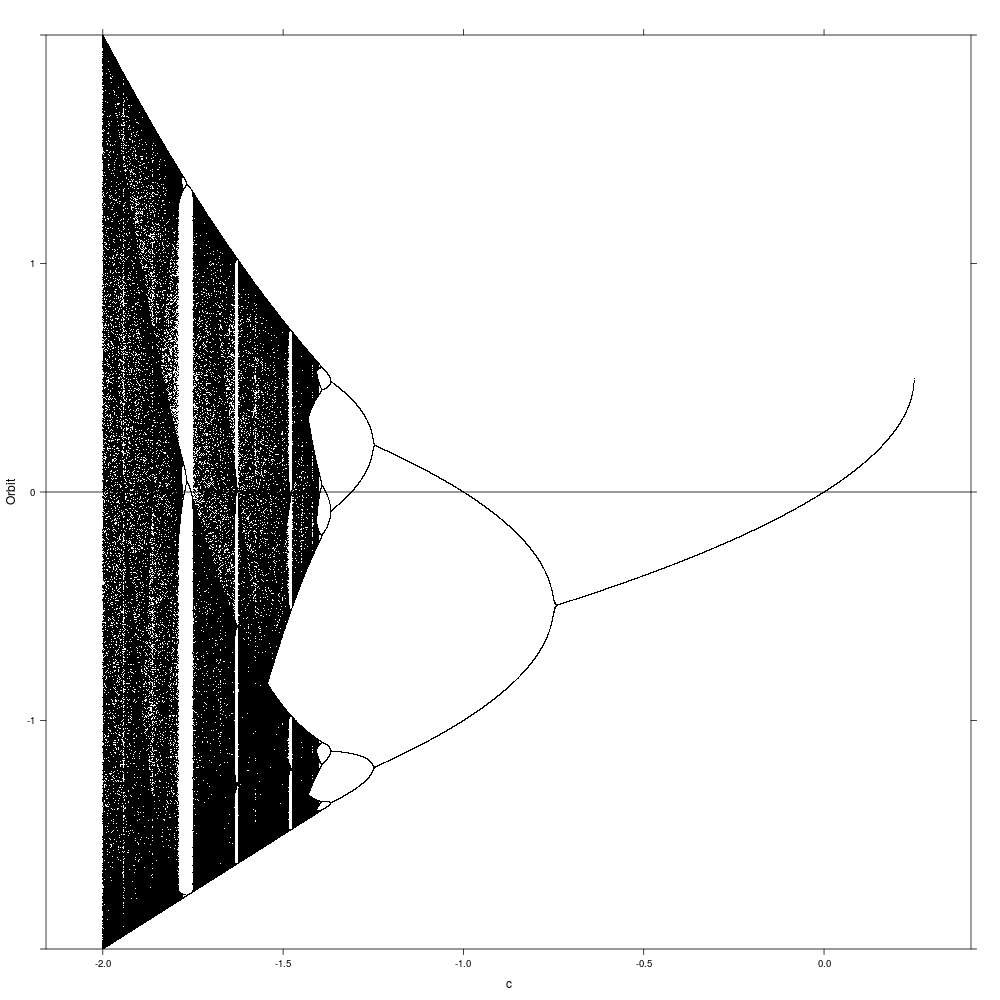
\includegraphics[width=\textwidth]{./img/orig}
				\caption{Orbit diagram of $x^2 + c$}
				\label{stand}%
		\end{subfigure}
		\caption{Orbit diagrams of the original and perturbed systems}\label{fig:orbits}
	\end{figure}
\end{frame}

\begin{frame}
	\frametitle{Other Interesting Intervals}
	\begin{figure}[h]
	\centering
	\begin{subfigure}[b]{0.5\textwidth}
			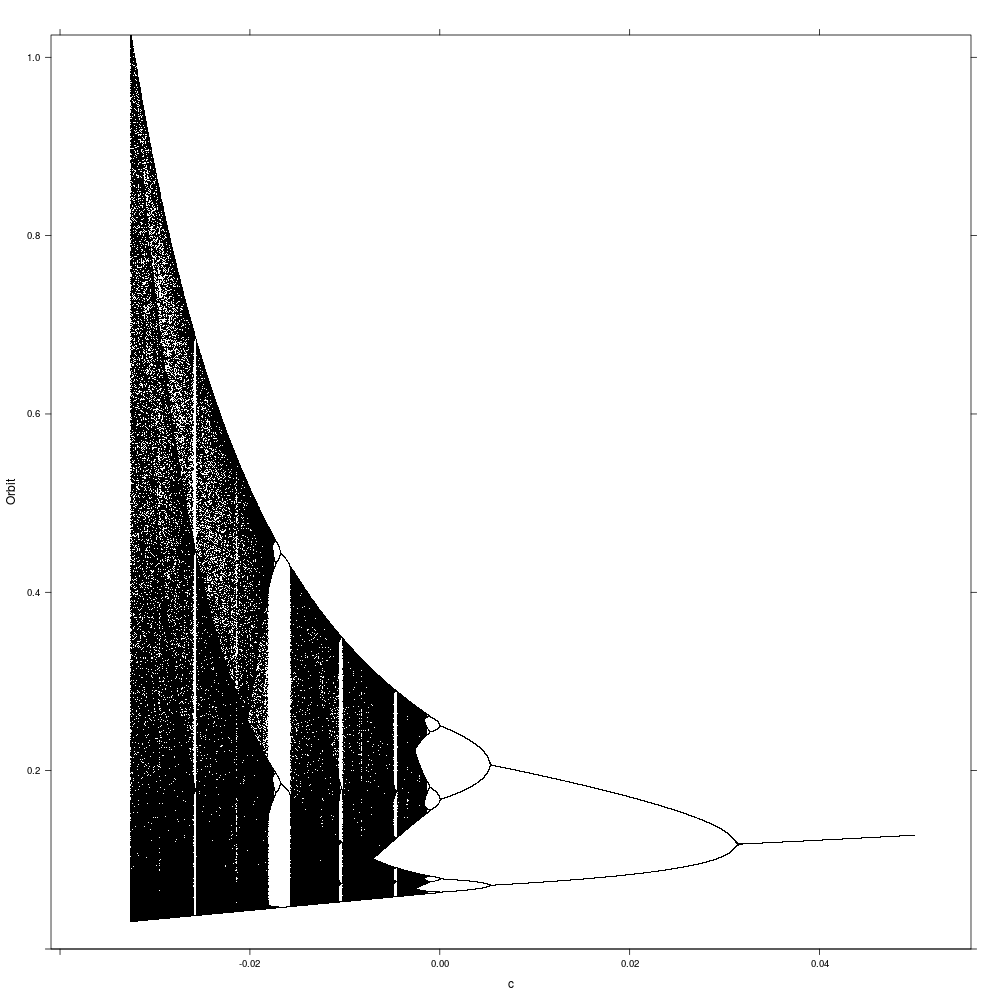
\includegraphics[width=\textwidth]{./img/pertperdub}
			\caption{Orbit Diagram for $Q_c (x)$ where $c\in (-.035, .05)$}
	\end{subfigure}%
	\begin{subfigure}[b]{0.5\textwidth}
			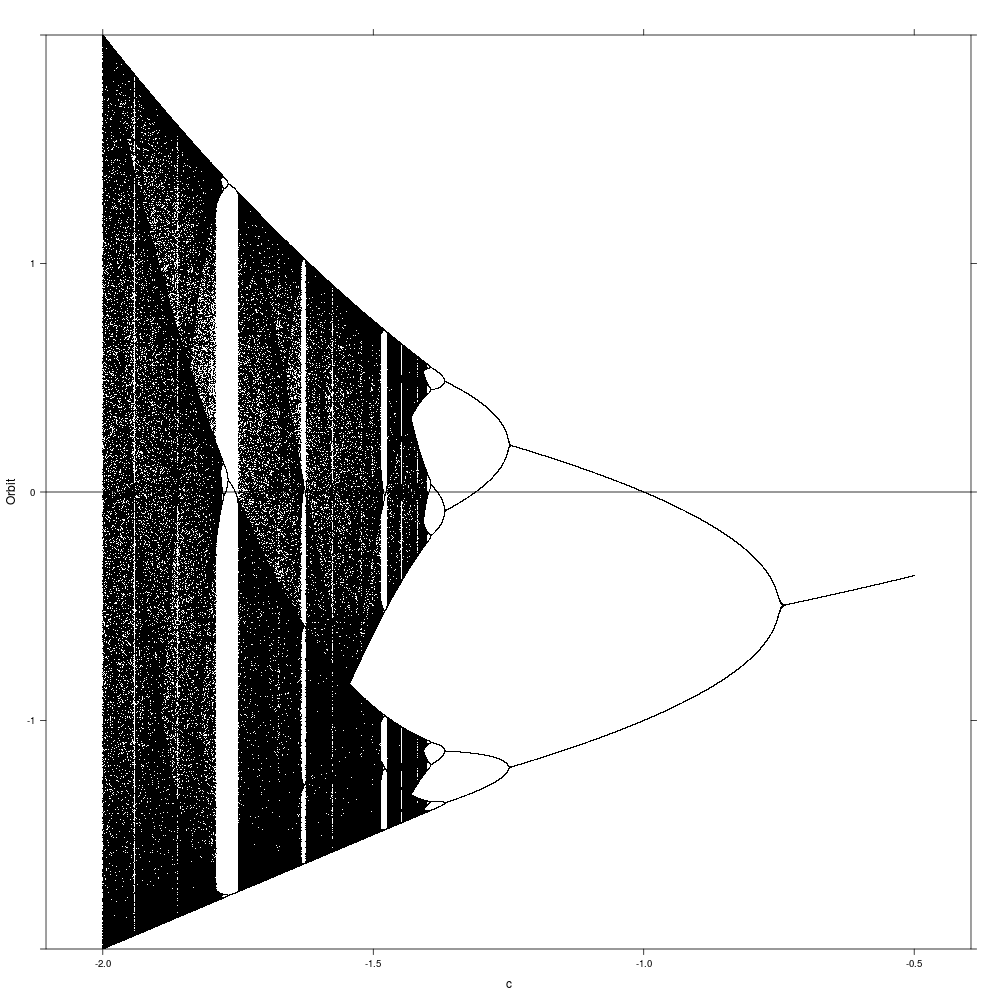
\includegraphics[width=\textwidth]{./img/stdperdub}
			\caption{Orbit Diagram for $Q_c (x)$ where $c\in (-2, -.5)$}
	\end{subfigure}
	\caption{Orbit diagrams of the original and perturbed systems}\label{fig:perdub}
\end{figure}
\end{frame}
\begin{frame}
	\frametitle{Zoom on Important Interval}
	\begin{figure}
			\includegraphics[width = \textwidth]{./img/over_plain}
			%\caption{Zoom on $x^2 + c + \frac{.001}{x^2}$ for $c \in (-.24,.09)$}
	\end{figure}
\end{frame}

\begin{frame}{Orbit Codings}
	\begin{figure}
		\centering
		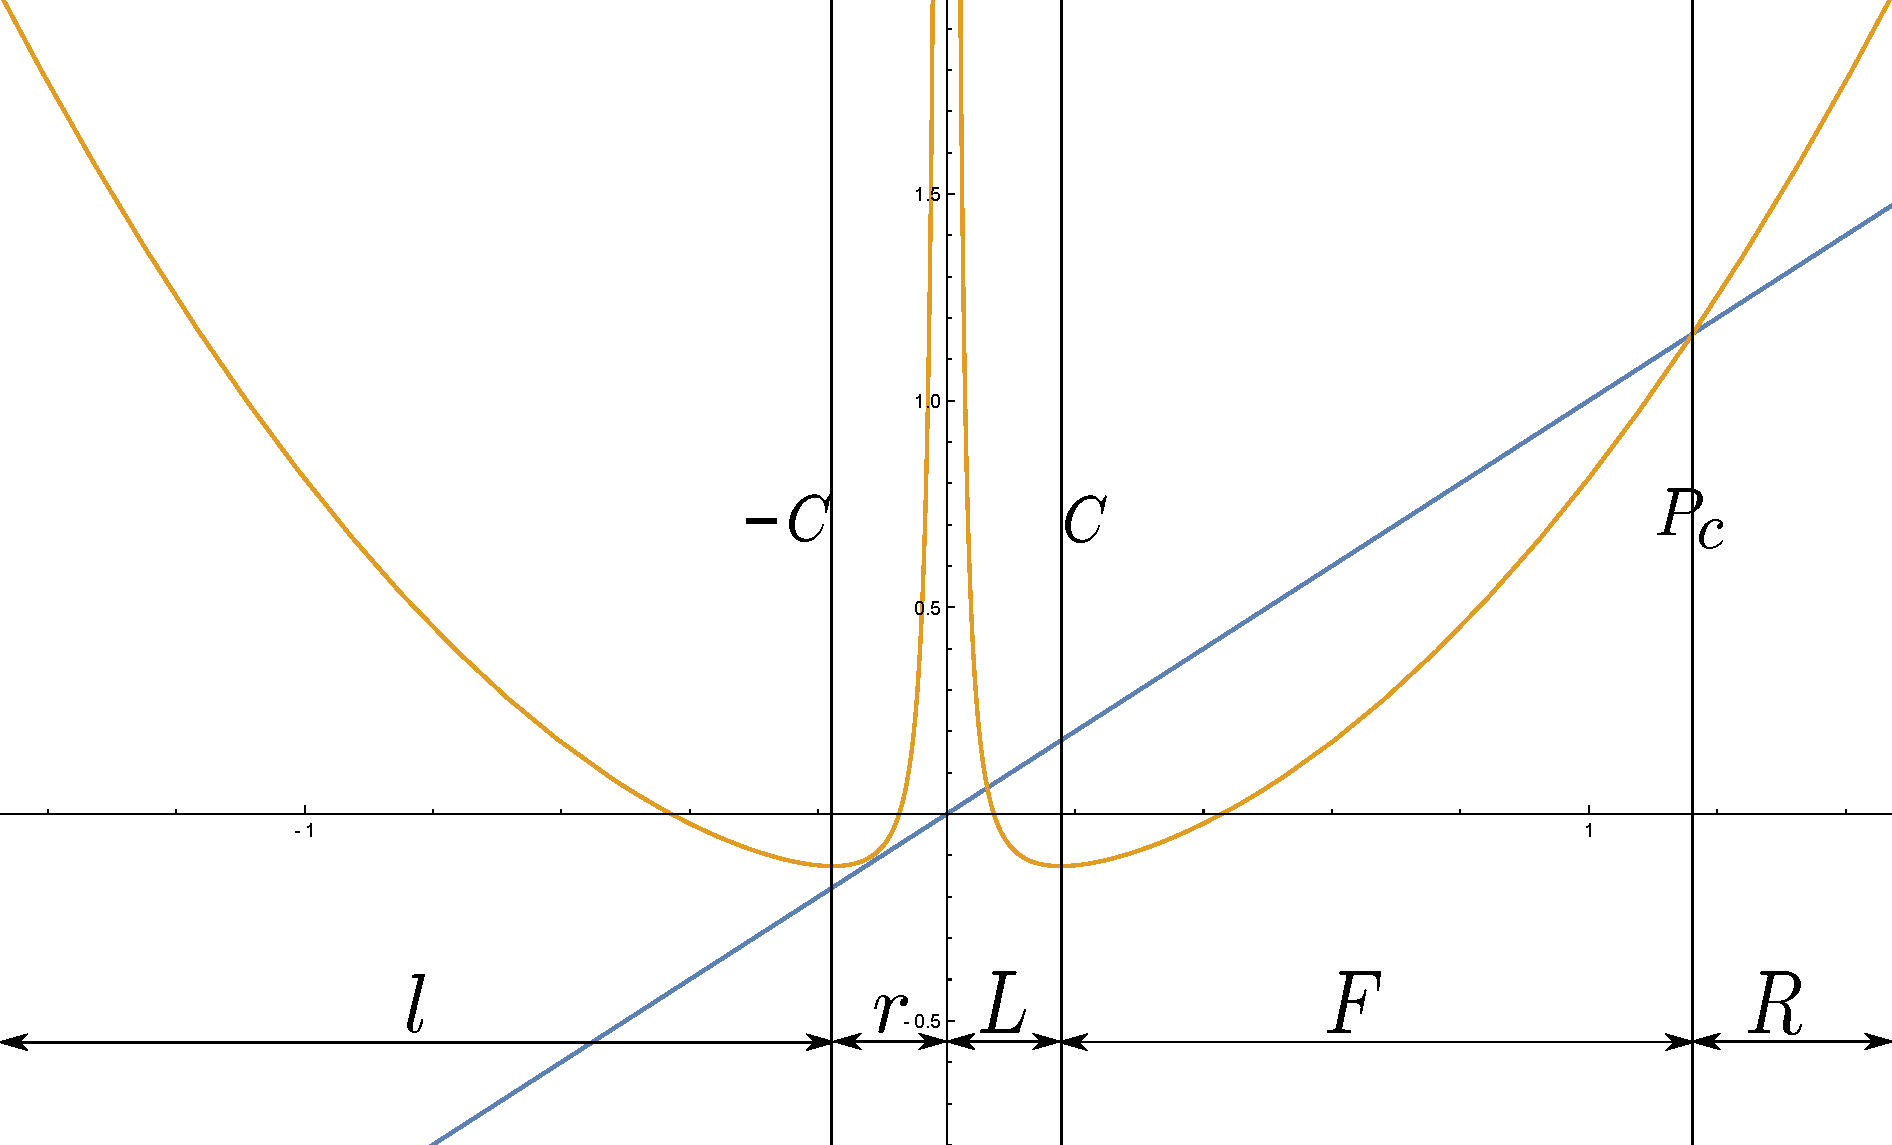
\includegraphics[width=.8\textwidth]{./img/codings}
		\caption{A partitioning of $\R$ into the intervals $l, r, L, F, R$}
	\end{figure}
\end{frame}

\begin{frame}{Example of Orbit Coding}
	\begin{figure}[h]
		\centering
		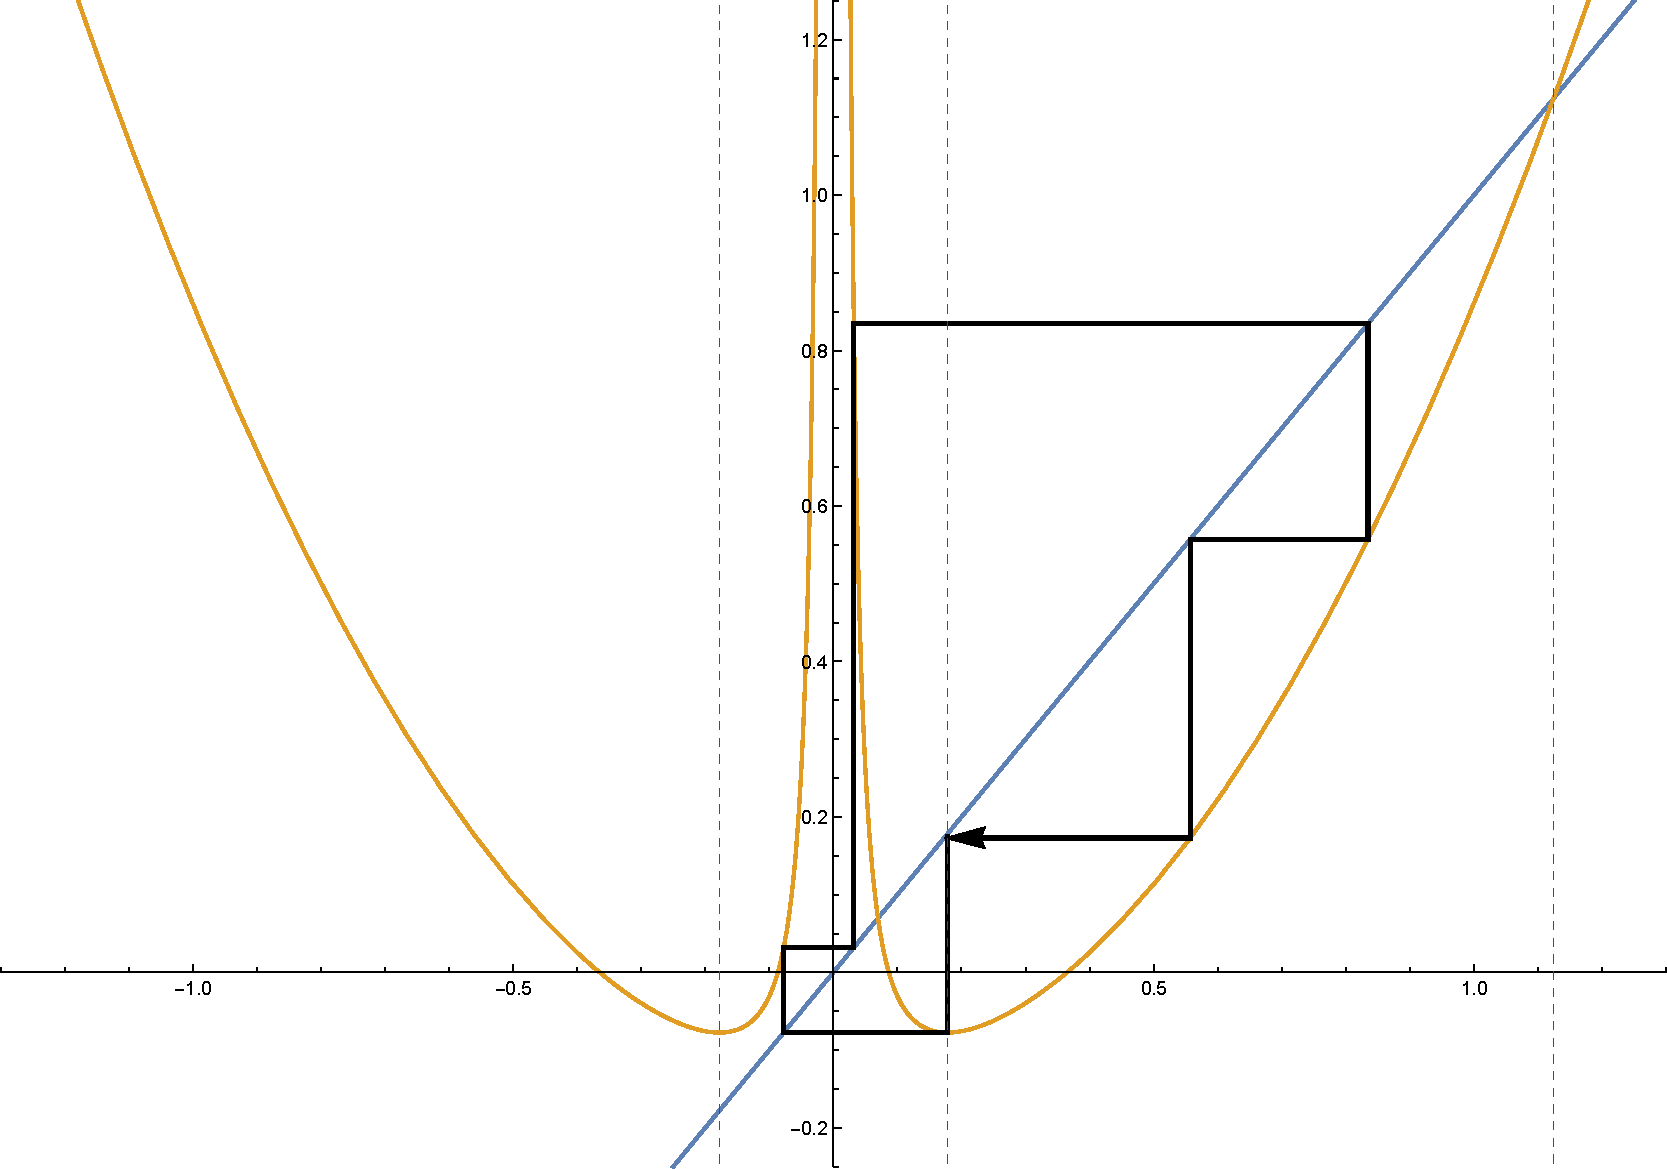
\includegraphics[width=.8\textwidth]{./img/orbitex}
		\caption{Graphical Iteration an periodic orbit with coding $CrLFFC$}
	\end{figure}
\end{frame}

\begin{frame}{Special Notation}
\begin{itemize}
		\item Let $C$ be the positive critical point
		\item Let $P_c$ be the right most fixed point (when it exists)
		\item Let $h_n$, $p_n$, $z_n$ be parameter values such that $f^n_{h_n} (C) = P_c$ (roughly corresponding to a homoclinic parameter value), $f^n_{p_n} (C) = C$ (corresponding to a superattracting periodic orbit parameter value), and $f^n_{z_n} (C) = 0$ (corresponding to a prezero parameter value) %Note that the solutions to these equations are typically not unique, we will refer to a specific parameter value with the coding of the critical orbit at that point by placing the coding at that parameter value in the superscript. For example, in Figure \ref{itright} we see graphical iteration of the critical point at the parameter value $\pr$ where we refer to the specific $h_2$ by listing the coding $CrP_c$
		\item Let $s_n$ be a parameter value where the $n^{th}$ iterate goes through a saddle node bifurcation
	\end{itemize}
\end{frame}

\begin{frame}{Fixed Points}
	\begin{figure}
		\centering
		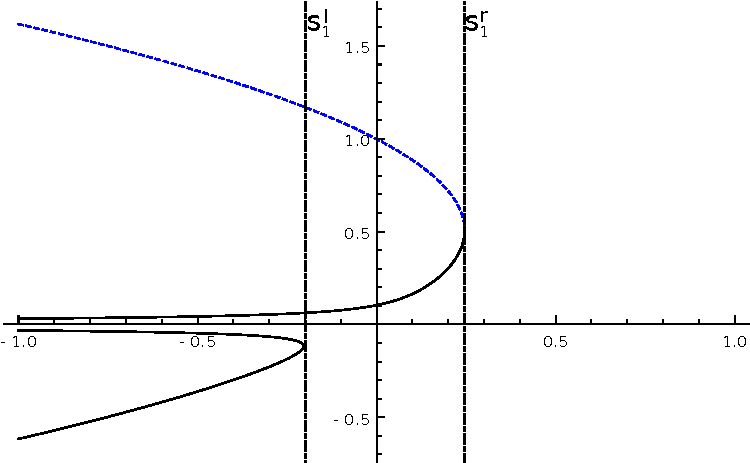
\includegraphics[width=.8\textwidth]{./img/pc}
		\caption{Plot of all of the fixed points of our system in parameter $\times$ phase space. The curve for $P_c$ is in blue/dashed}
	\end{figure}
\end{frame}

\subsection{Statement of 1-D Results}

\begin{frame}[allowframebreaks]{Statement of Results}
	% \frametitle{}
	\begin{proposition}
		On the interval $ (\pl, \pr)$, there is an accumulation of parameter values $p_n$ and $z_n$ which give critical orbit coding $CrF^{n-1}$ for any integer $n \geq 2$

		{\normalsize
		\[
		z_n < p_n < z_{n+1} < p_{n+1} < \cdots < h_2^{CrP_c}
		\]}

		The numerics suggest that the accumulation will limit to the point $h_2^{CrP_c}$.
	\end{proposition}
	\begin{proposition}
		On the interval $ (\pl, \pr)$, there is an accumulation of parameter values $p_n$, $z_n$, and $h_n$ which give critical orbit coding $Cr^{n-2}$ for any integer $n \geq 2$ such that

		{\normalsize 
		\[
		s^l_1 < \cdots < z_{n+1} < p_{n+1} < h_{n+1} < z_n < p_n < h_n
		\]}

		The numerics suggest that the accumulation will limit to the point $s^l_1$.
	\end{proposition}
\end{frame}


\begin{frame}{Plot of Critical Point}
	\begin{figure}
		\centering
		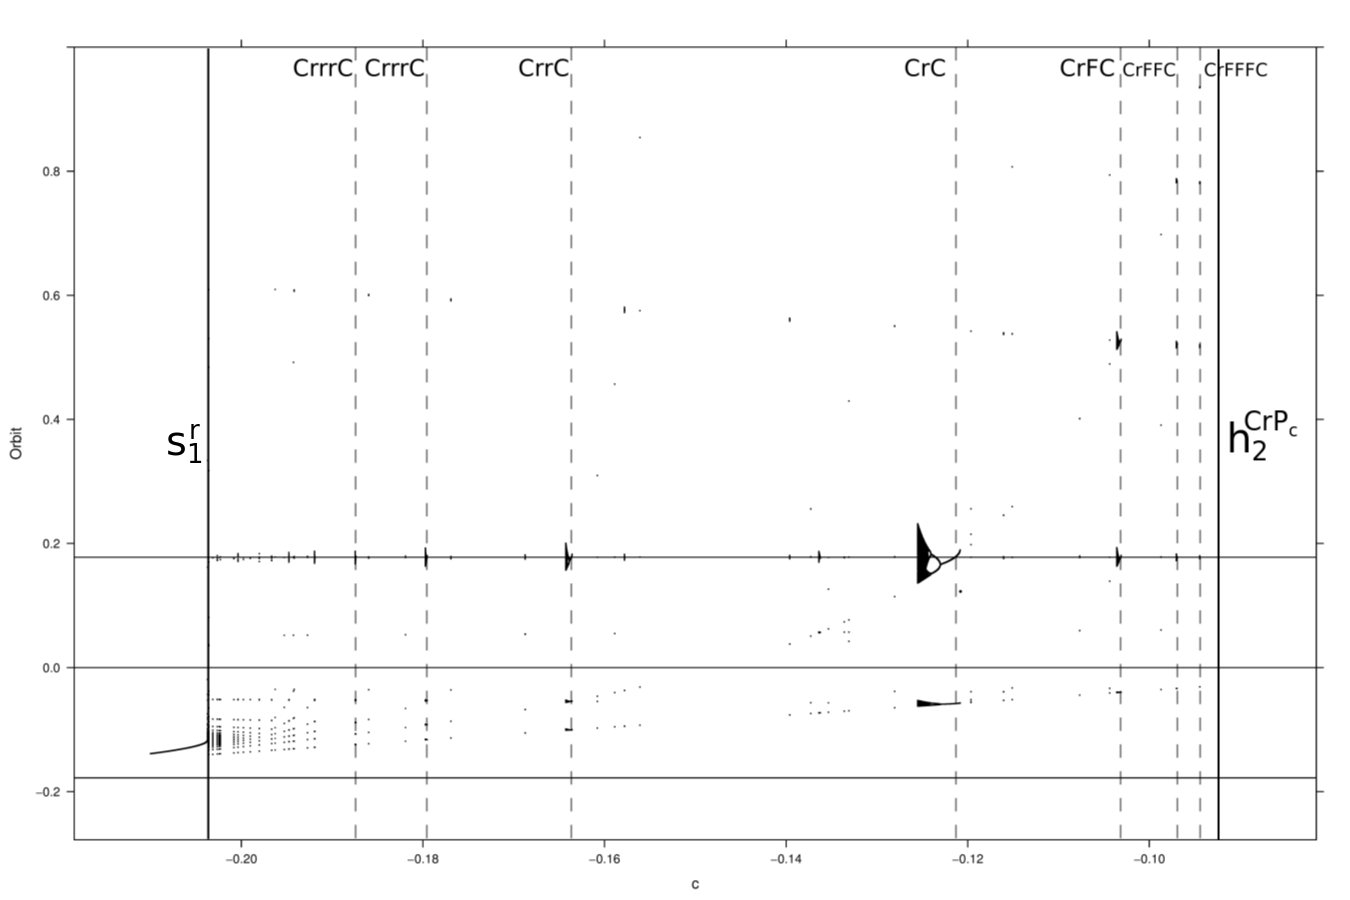
\includegraphics[width=.8\textwidth]{./img/over.png}
		\caption{Orbit Diagram for $x^2 + c + \frac{.001}{x^2}$}
	\end{figure}
\end{frame}



\subsection{Graphical Intuition}

\begin{frame}{Plot of Critical Point}
	\begin{figure}
		\centering
		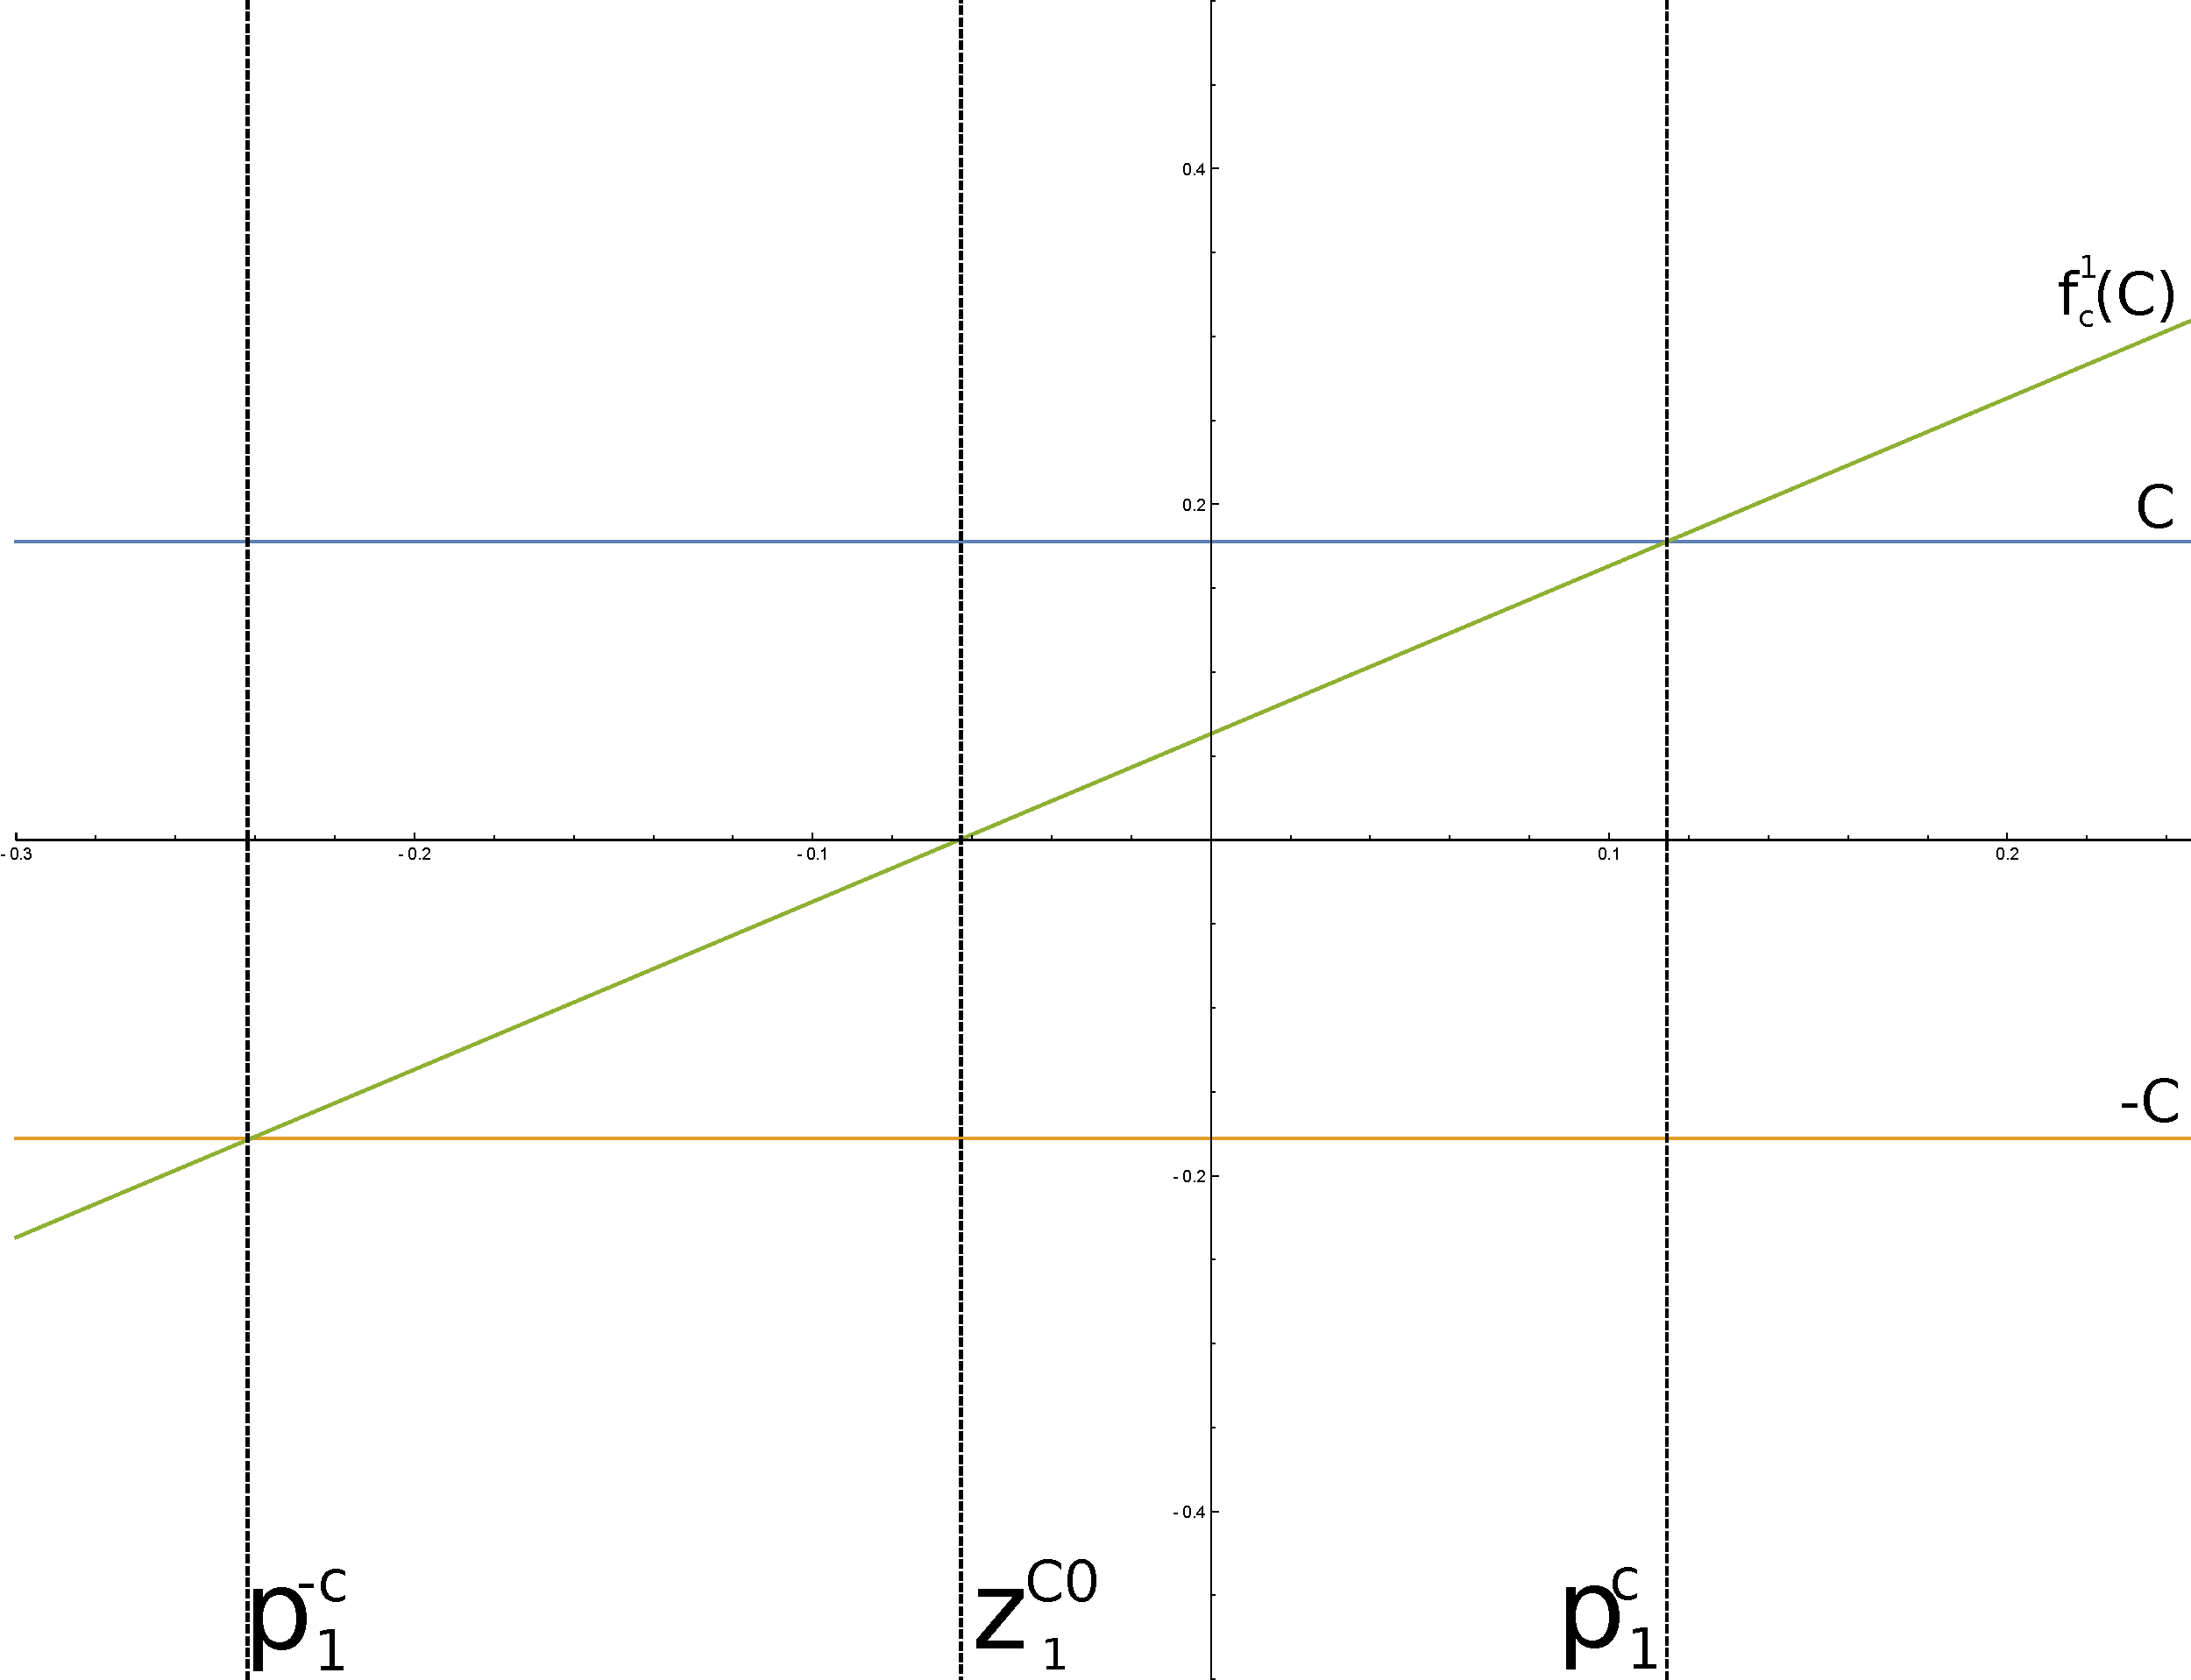
\includegraphics[width=.8\textwidth]{./img/1it}
		\caption{Plot of $f^1_c (C)$ for $c \in (-.3,.246)$}
	\end{figure}
\end{frame}

\begin{frame}{Graphical Iteration}
	\begin{figure}[h]
		\centering
		\begin{subfigure}[b]{0.4\textwidth}
				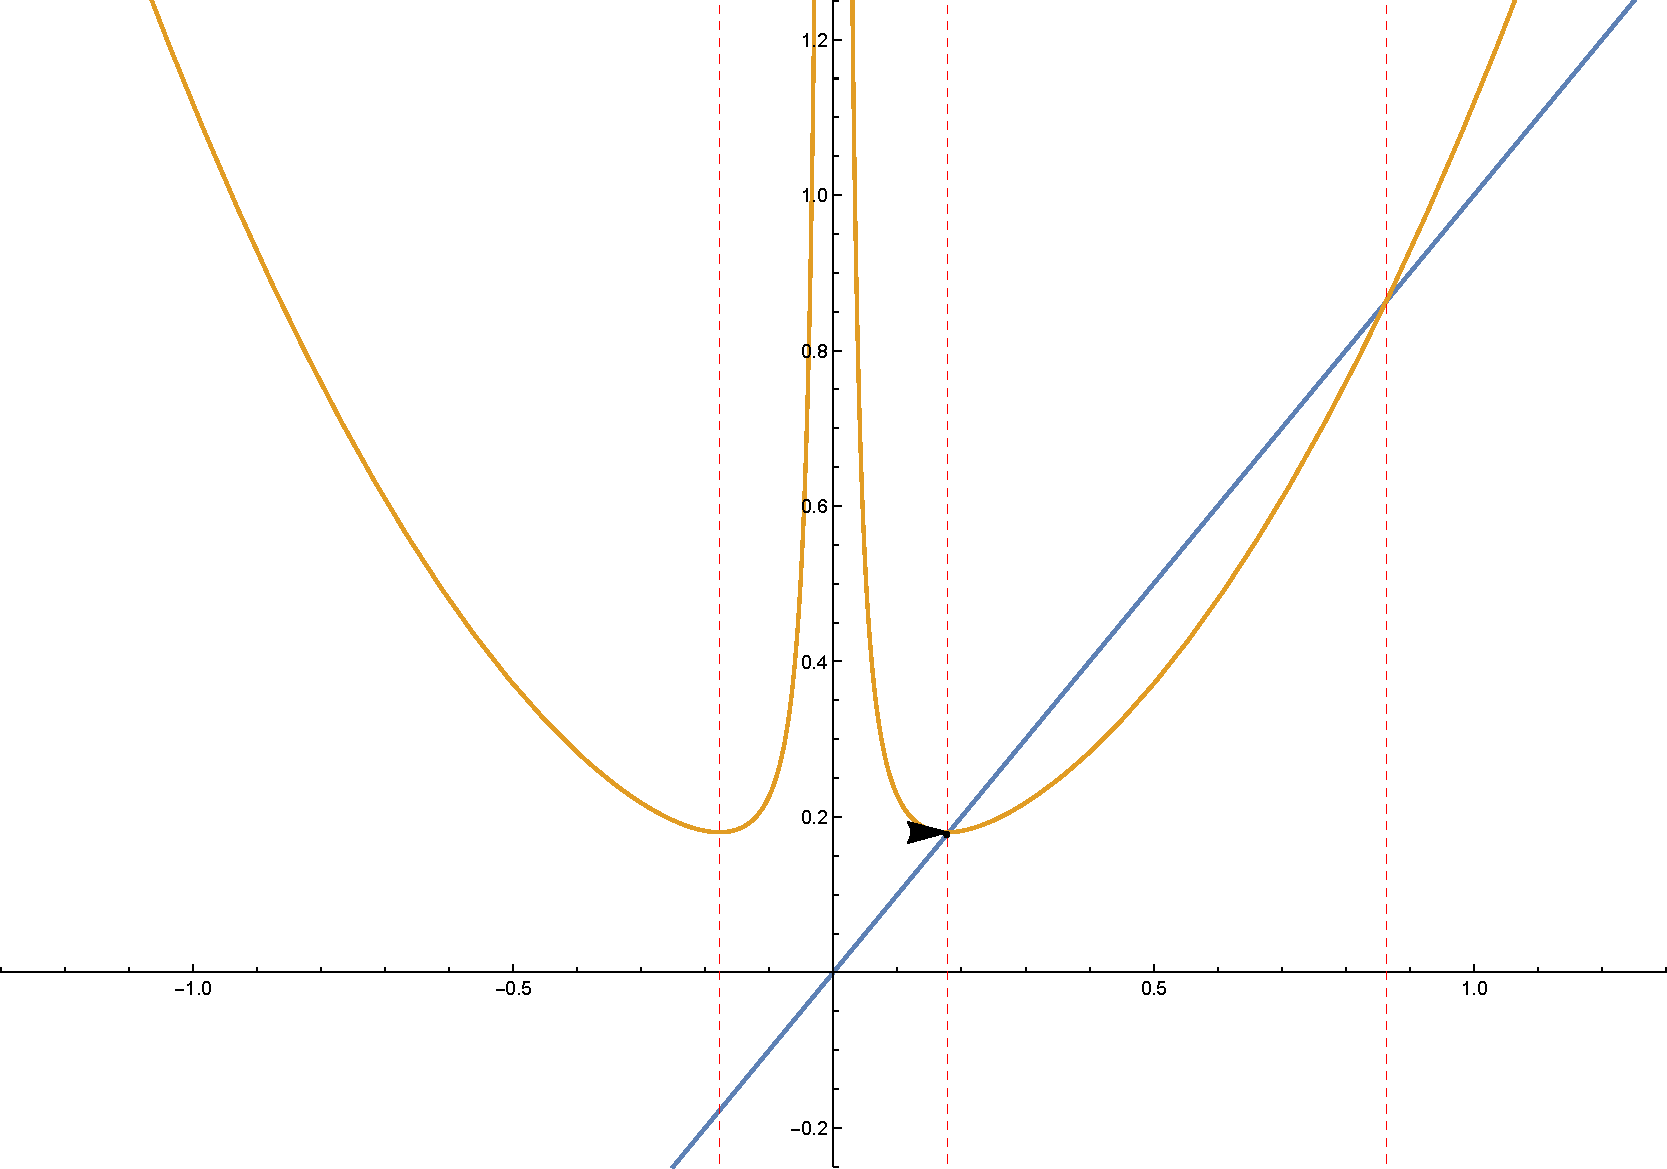
\includegraphics[width=\textwidth]{./img/it1-1}
				\caption{$c \approx p_1^{C}$}
		\end{subfigure}%
		\begin{subfigure}[b]{0.4\textwidth}
				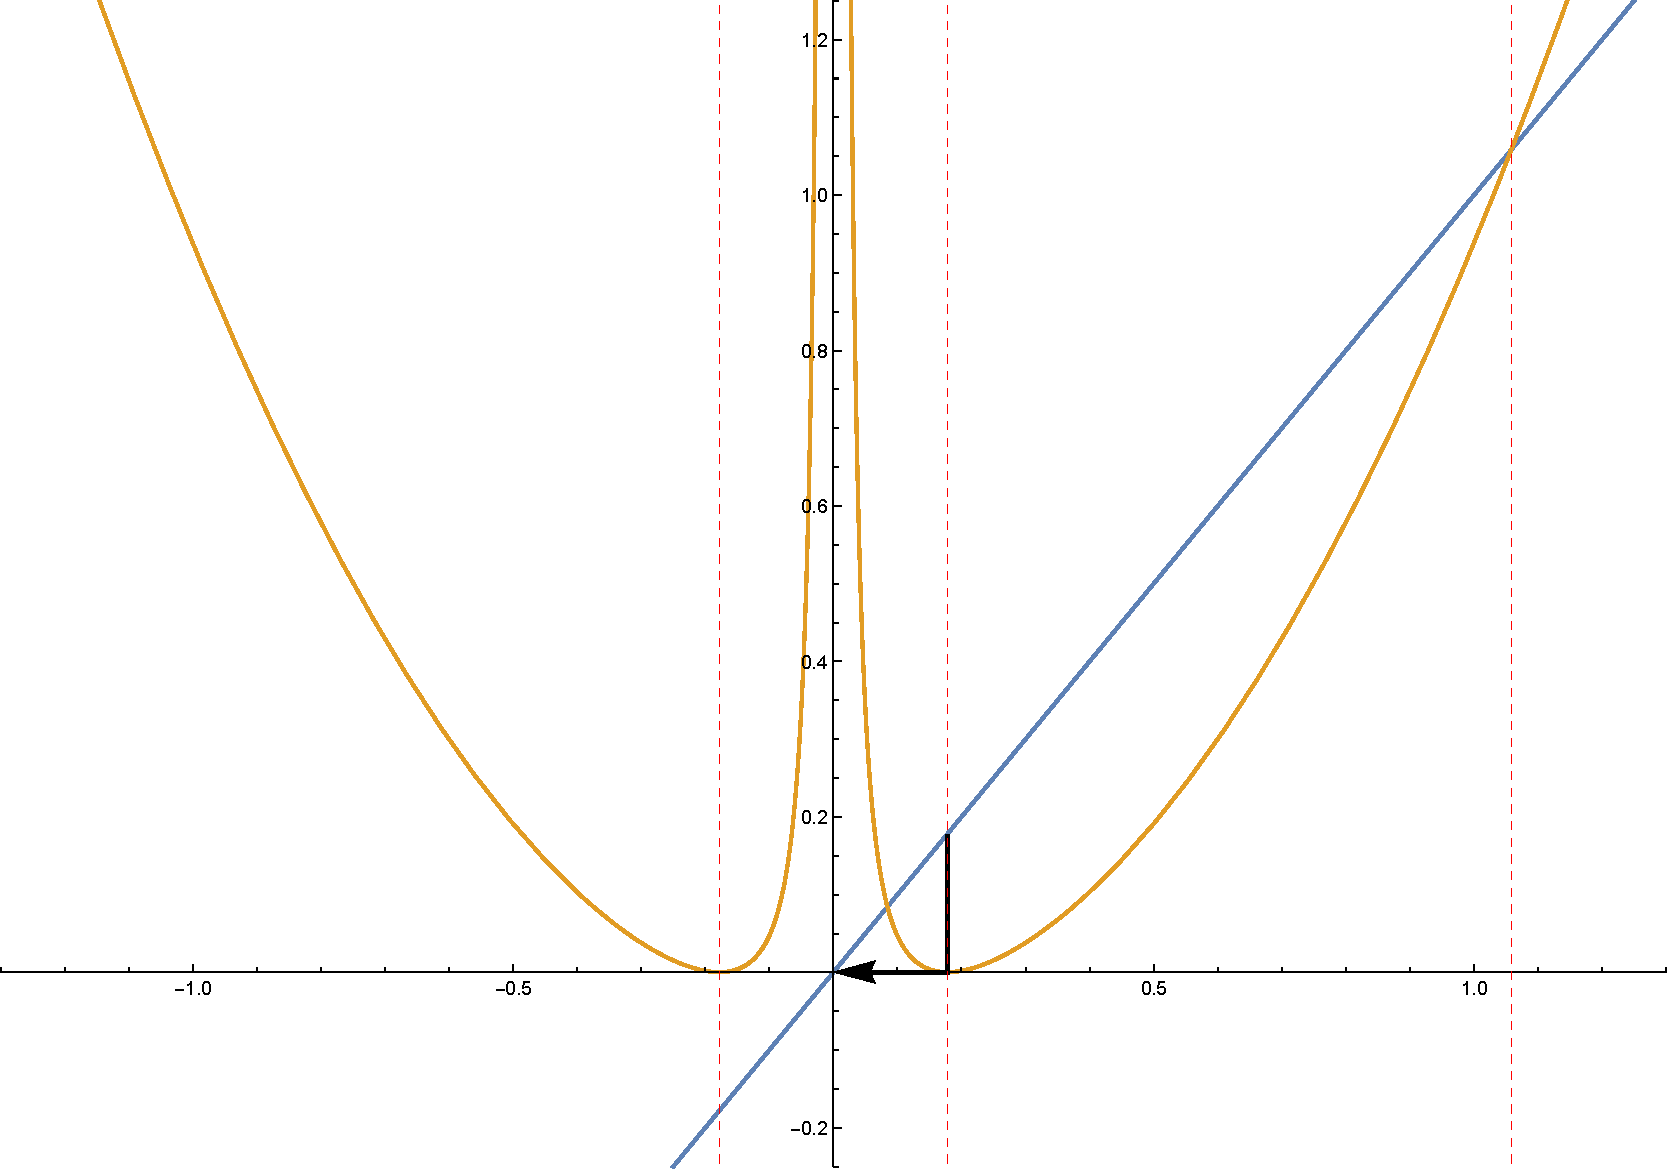
\includegraphics[width=\textwidth]{./img/it1-2}
				\caption{$c \approx z_1^{C0}$}
		\end{subfigure}
		\begin{subfigure}[b]{0.4\textwidth}
				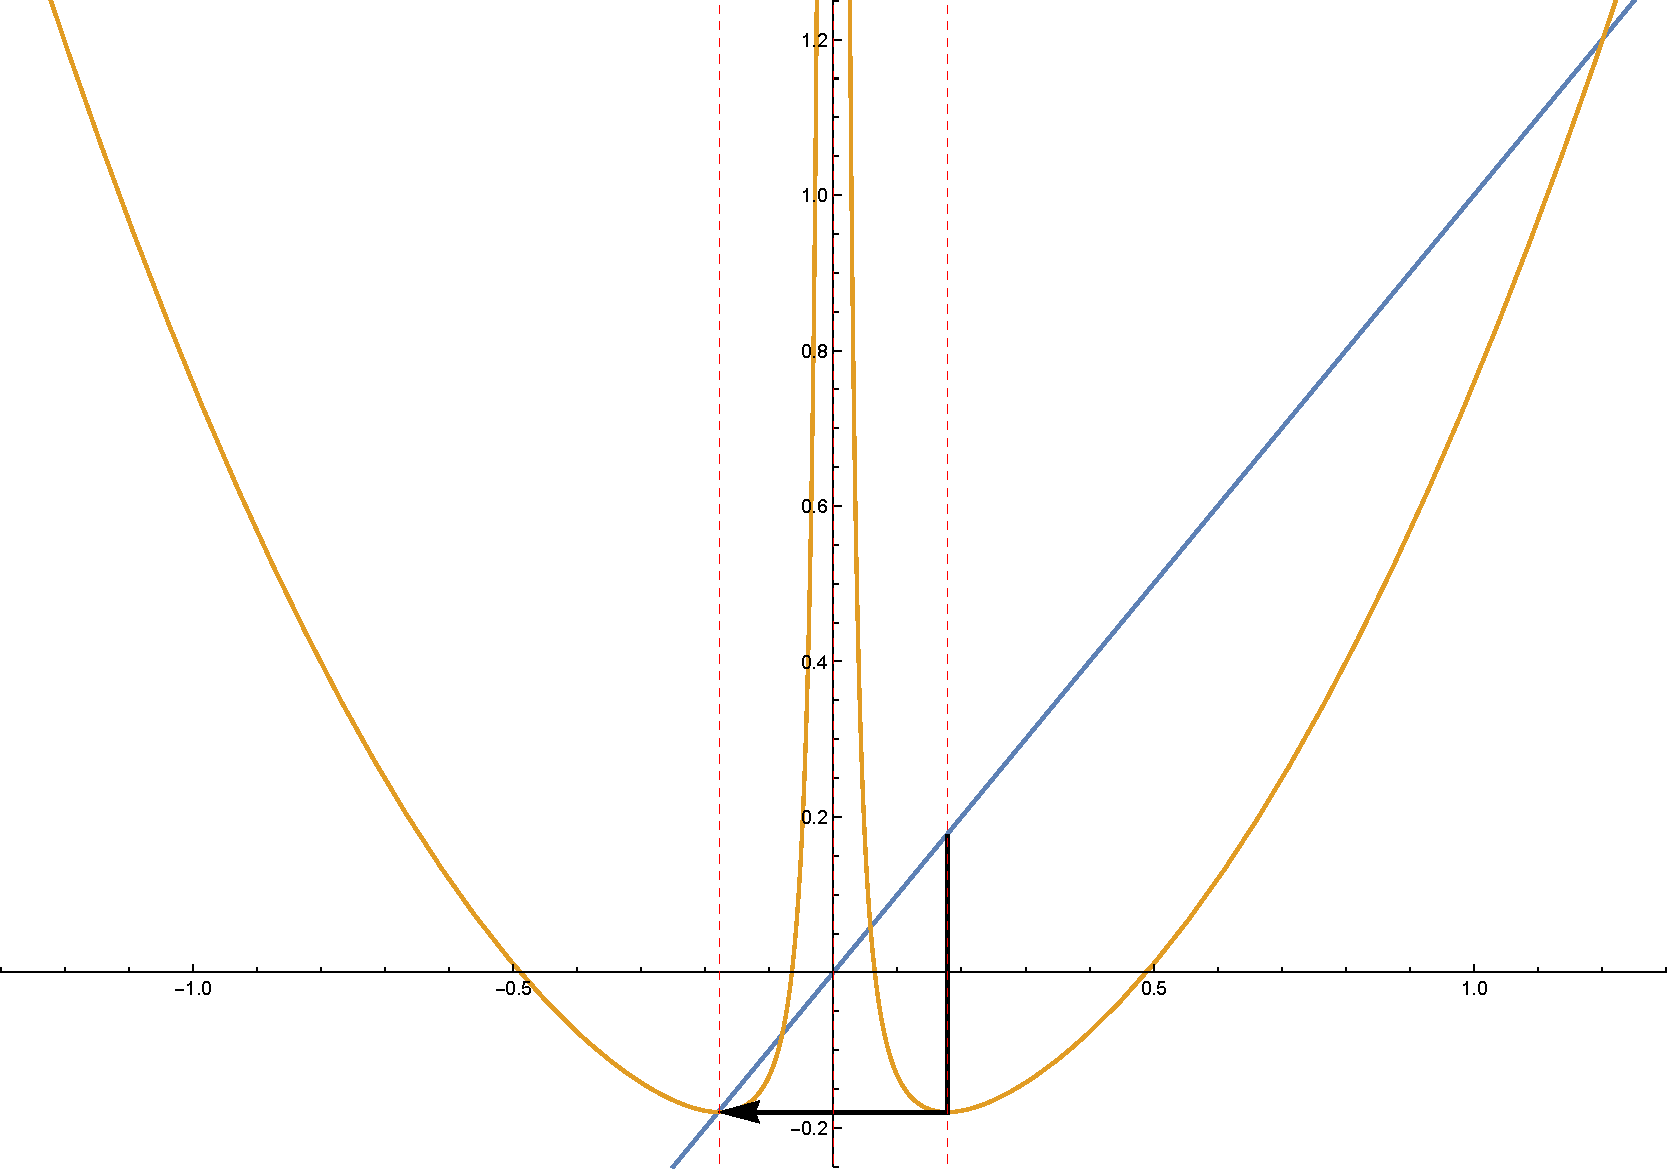
\includegraphics[width=\textwidth]{./img/it1-3}
				\caption{$c \approx p_1^{-C}$}
		\end{subfigure}
		% \caption{Orbit diagrams of the original and perturbed systems}\label{fig:perdub}
	\end{figure}
\end{frame}



\begin{frame}{Plot of Critical Point}
	\begin{figure}
		\centering
		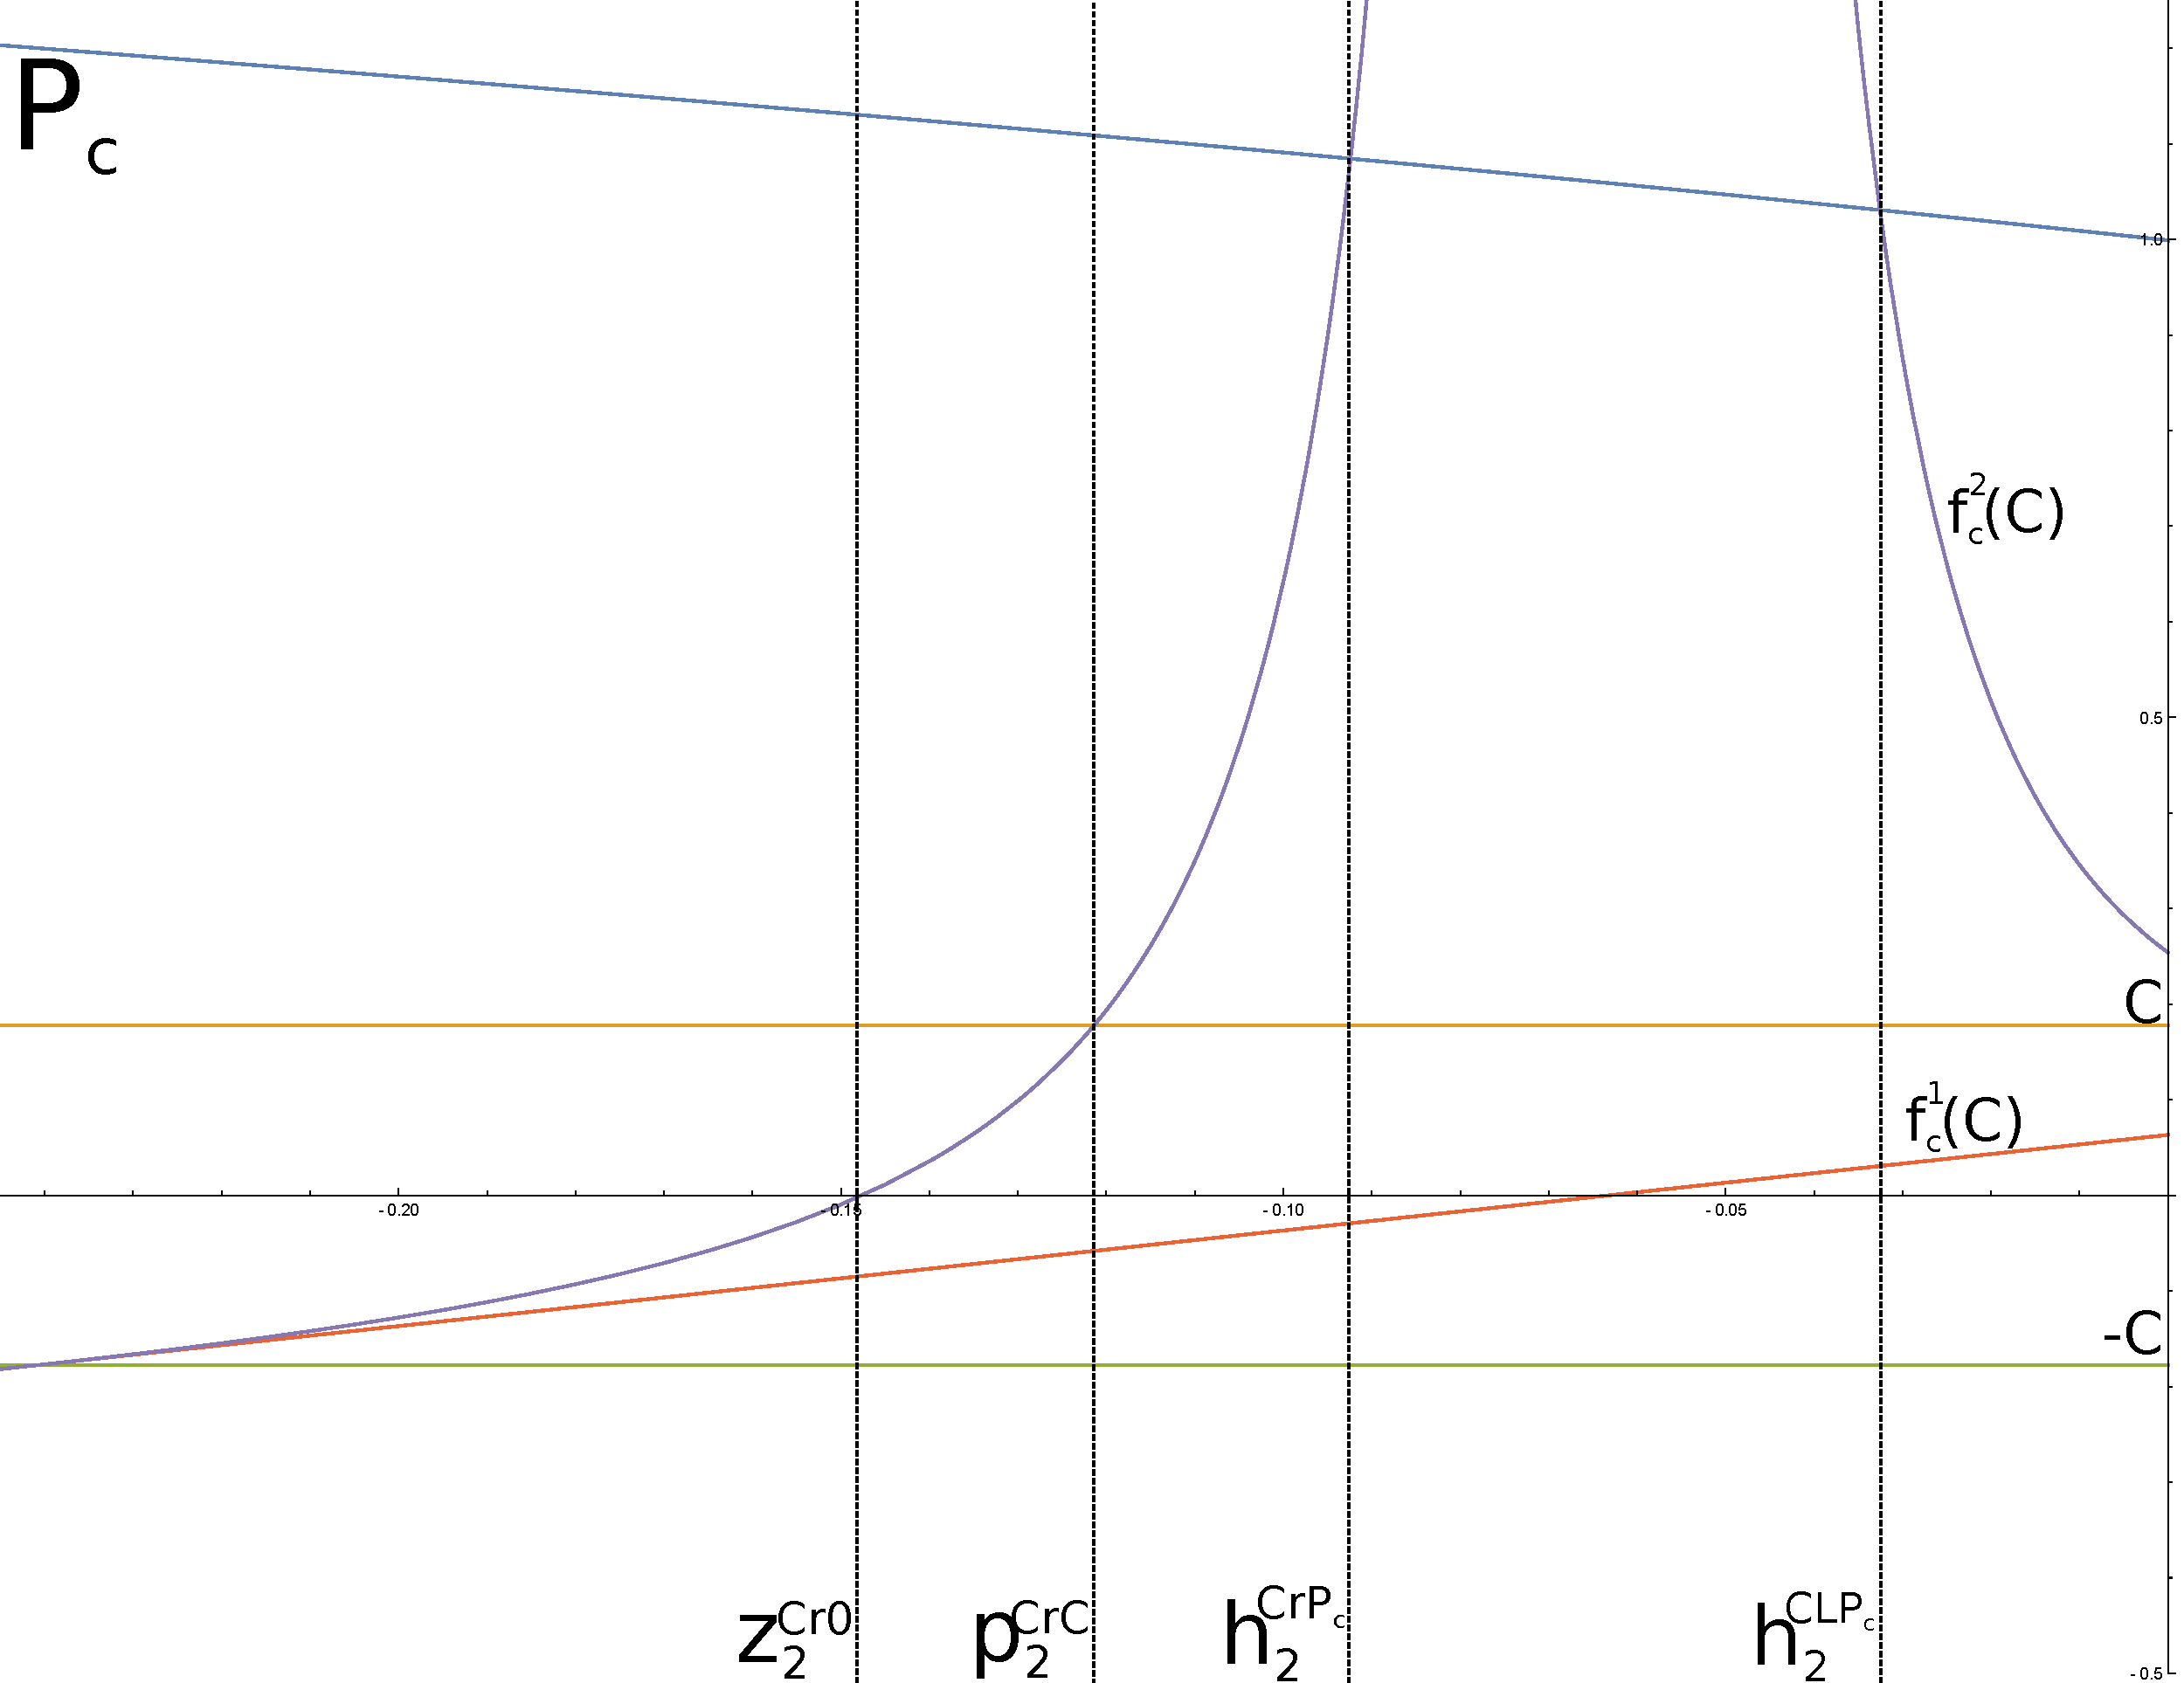
\includegraphics[width=.8\textwidth]{./img/2it}
		\caption{Plot of $f^1_c (C)$ and $f^2_c (C)$ for $c \in (-.245,0)$}
	\end{figure}
\end{frame}

\begin{frame}{Graphical Iteration}
	\begin{figure}[h]
		\centering
		\begin{subfigure}[b]{0.4\textwidth}
				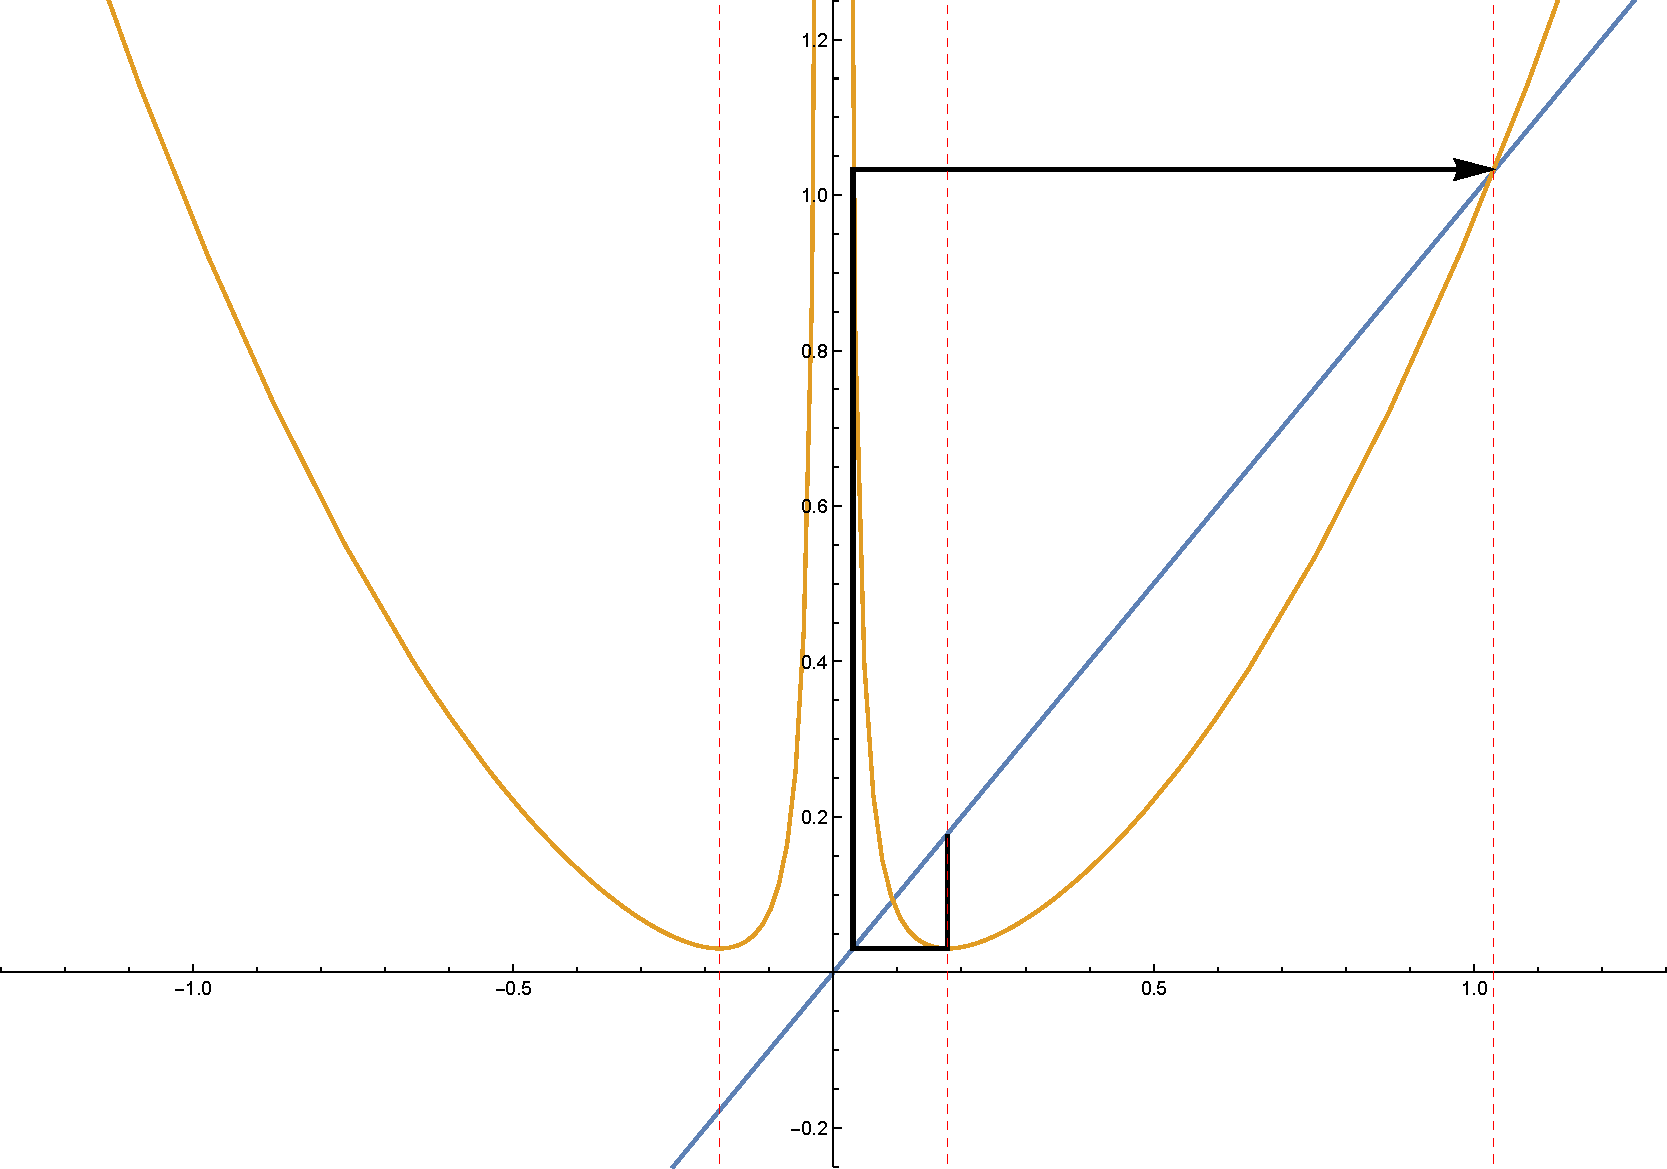
\includegraphics[width=\textwidth]{./img/it2-1}
				\caption{$c \approx h_2^{CLP_c}$}
		\end{subfigure}%
		\begin{subfigure}[b]{0.4\textwidth}
				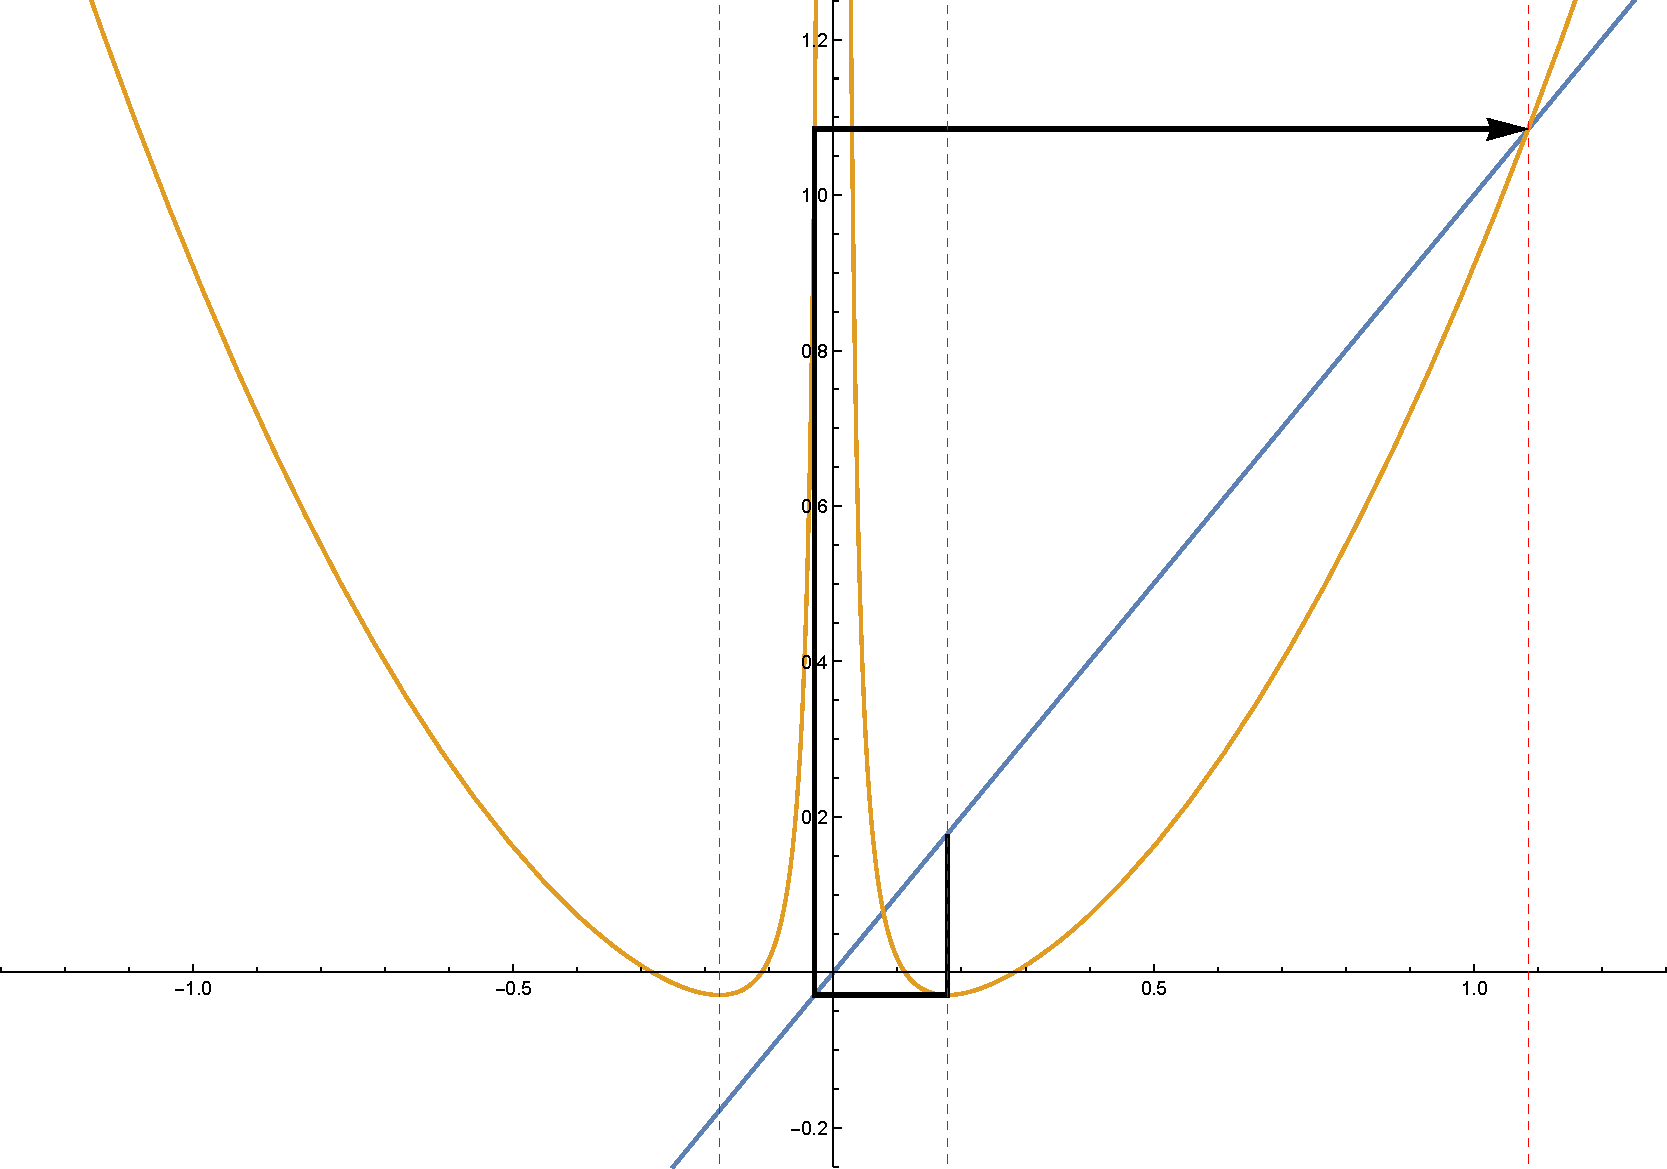
\includegraphics[width=\textwidth]{./img/it2-2}
				\caption{$c \approx h_2^{CrP_c}$}
		\end{subfigure}
		\begin{subfigure}[b]{0.4\textwidth}
				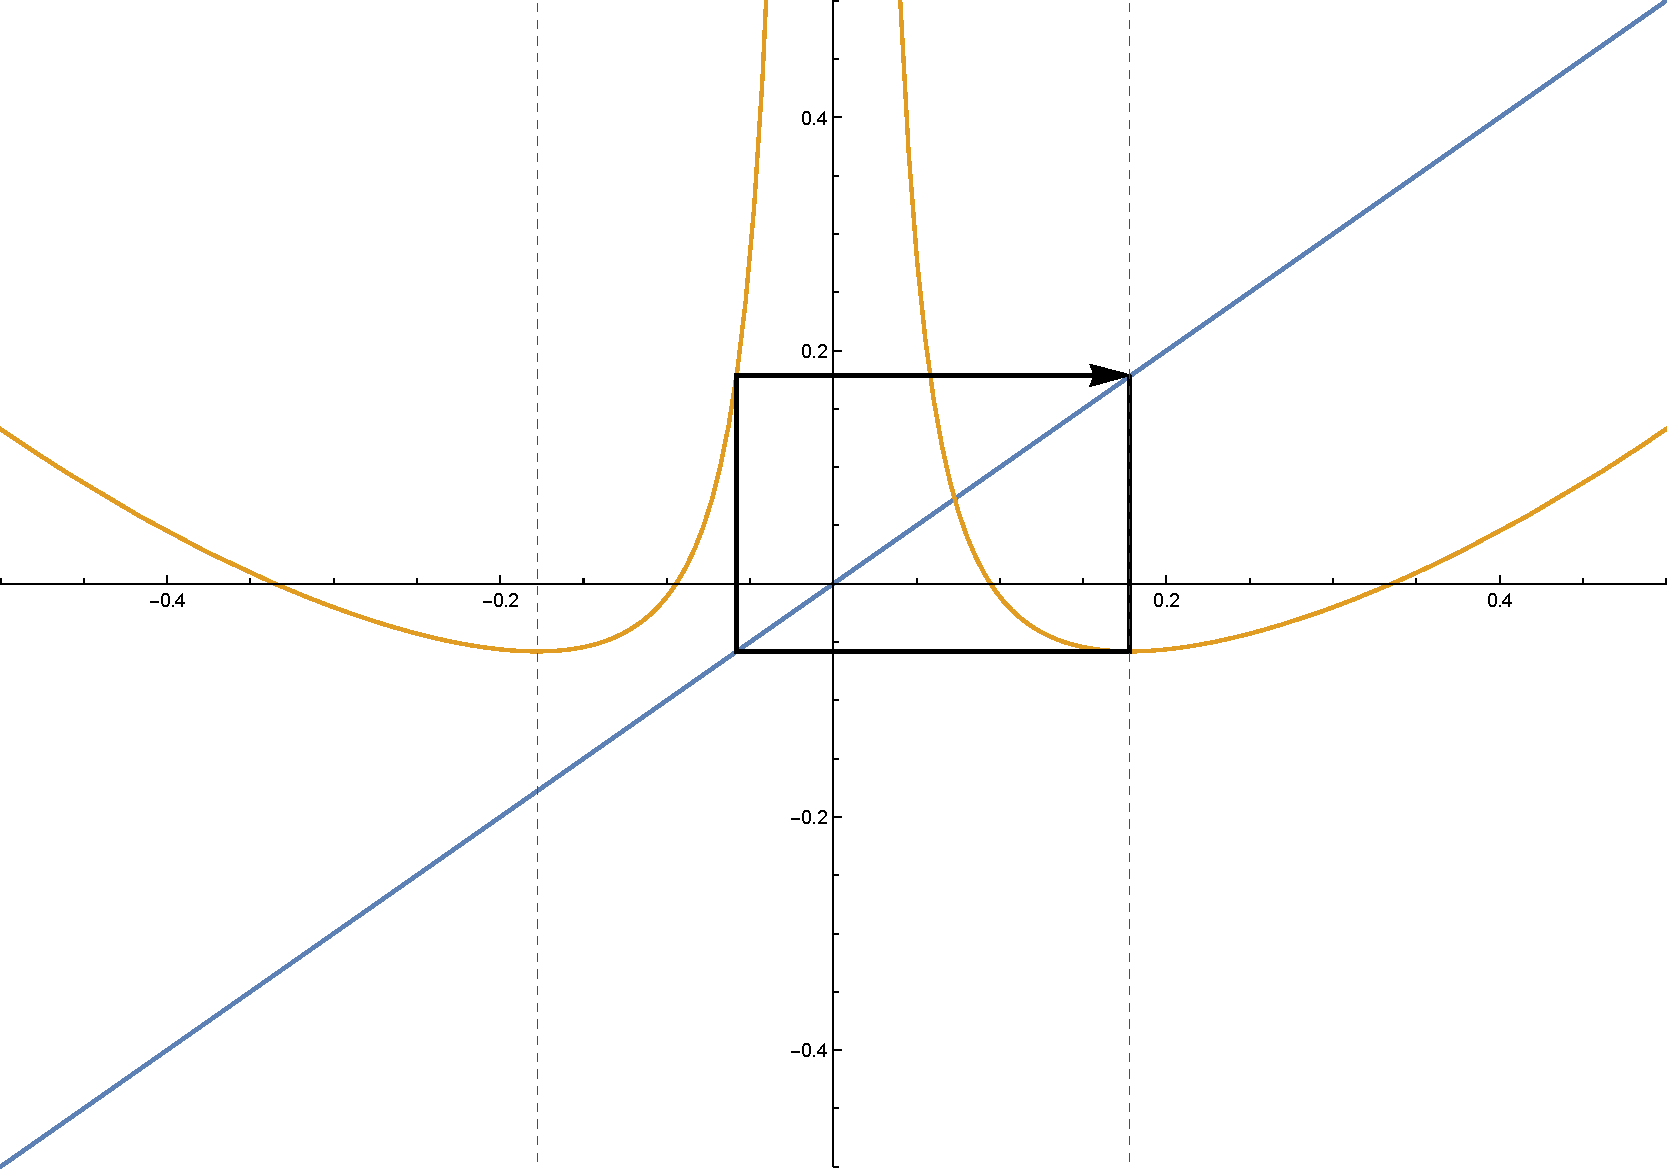
\includegraphics[width=\textwidth]{./img/it2-3}
				\caption{$c \approx p_2^{CrC}$}
		\end{subfigure}
		\begin{subfigure}[b]{0.4\textwidth}
			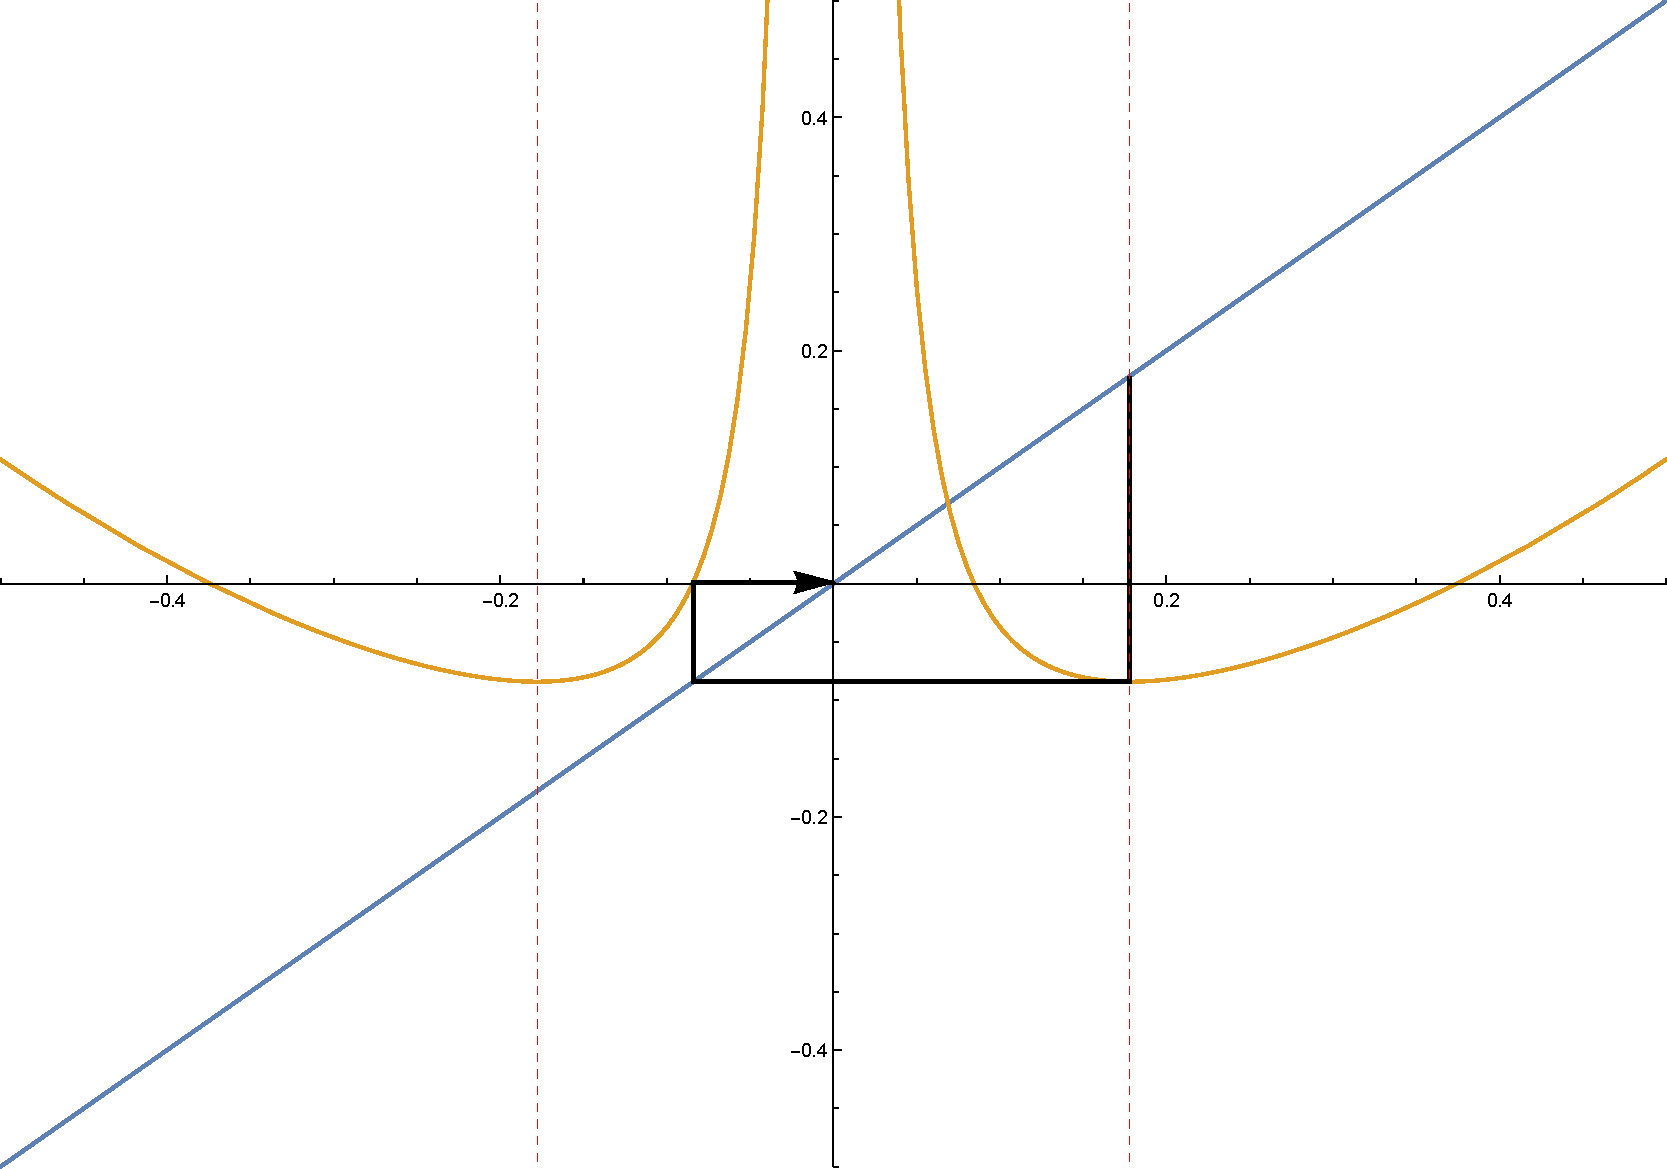
\includegraphics[width=\textwidth]{./img/it2-4}
			\caption{$c \approx z_2^{Cr0}$}
		\end{subfigure}
		% \caption{Orbit diagrams of the original and perturbed systems}\label{fig:perdub}
	\end{figure}
\end{frame}

\begin{frame}{Plot of Critical Point}
	\begin{figure}
		\centering
		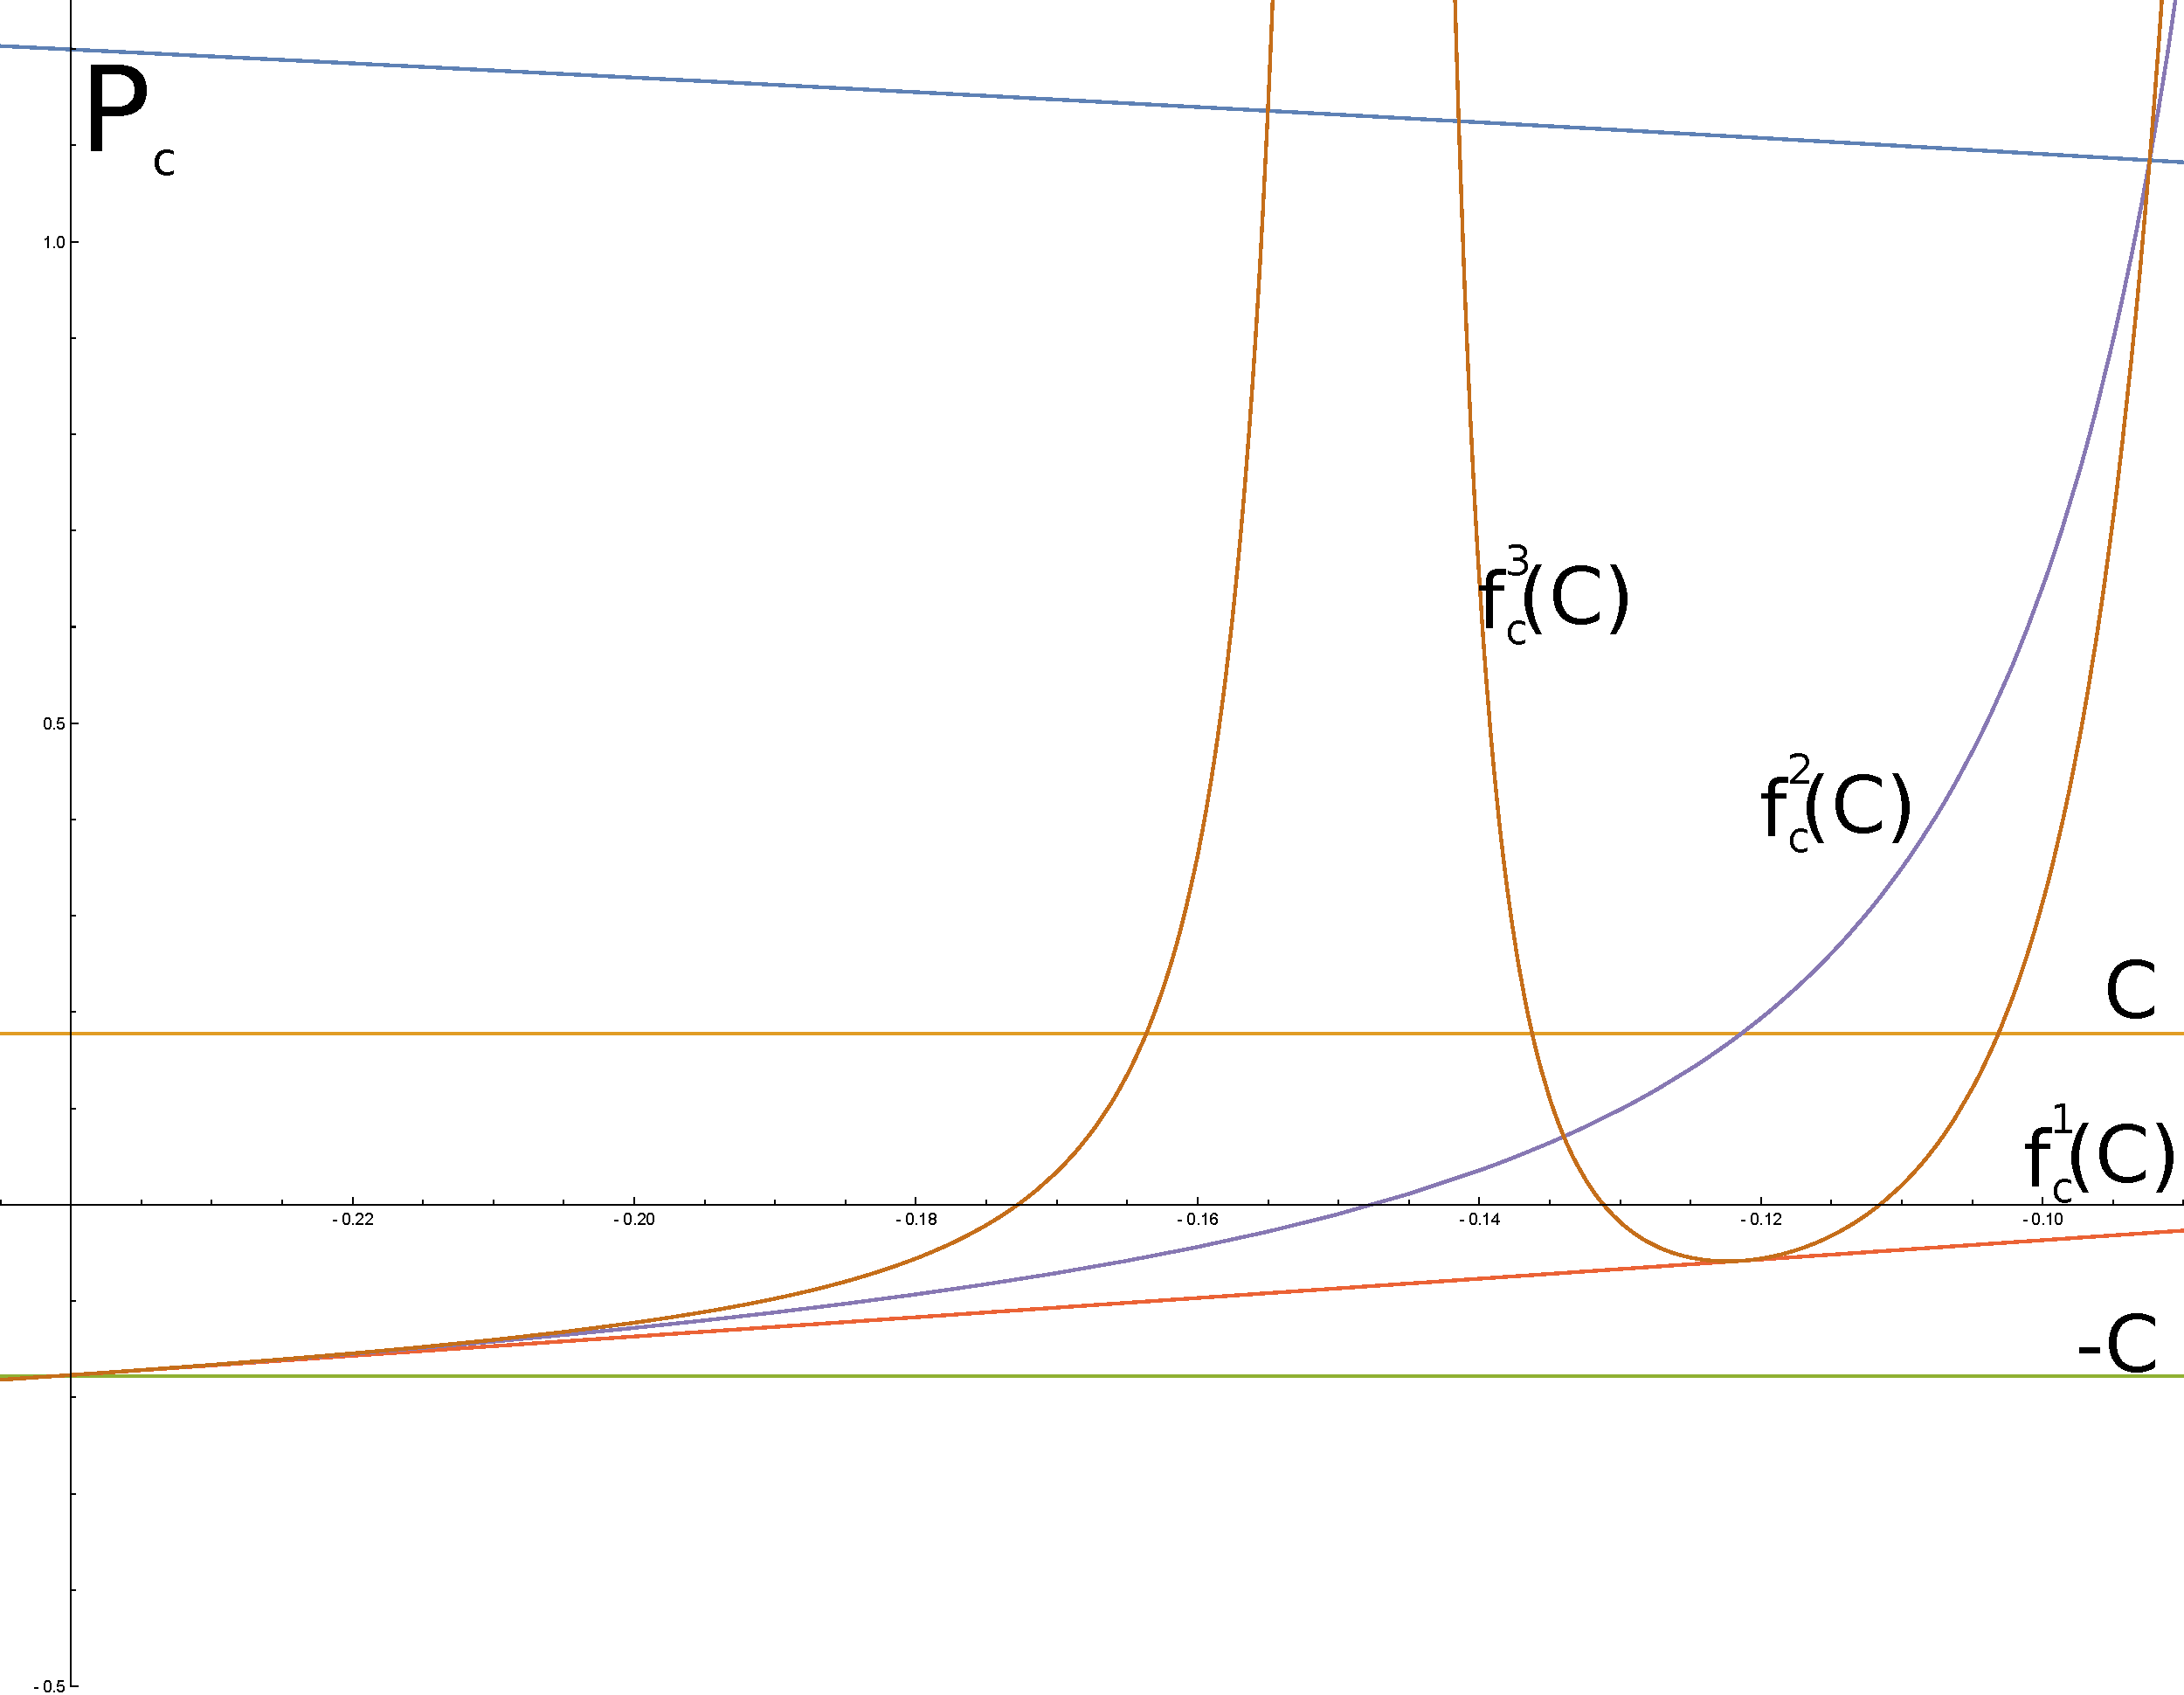
\includegraphics[width=.8\textwidth]{./img/3it}
		\caption{\footnotesize Plot of $f^1_c (C),f^2_c (C),f^3_c (C)$ for $c \in (-.245,-0.09) \approx (\pl,\pr)$}
	\end{figure}
\end{frame}

\begin{frame}{Right Hand Accumulation}
	% \frametitle{}
	\begin{proposition}
		On the interval $ (\pl, \pr)$, there is an accumulation of parameter values $p_n$ and $z_n$ which give critical orbit coding $Cr^{n-2}$ for any integer $n \geq 2$
		\[
		z_n < p_n < z_{n+1} < p_{n+1}
		\]
		The numerics suggest that the accumulation will limit to the point $h_2^{CrP_c}$.
	\end{proposition}
\end{frame}

\begin{frame}{Plot of Critical Point}
	\begin{figure}
		\centering
		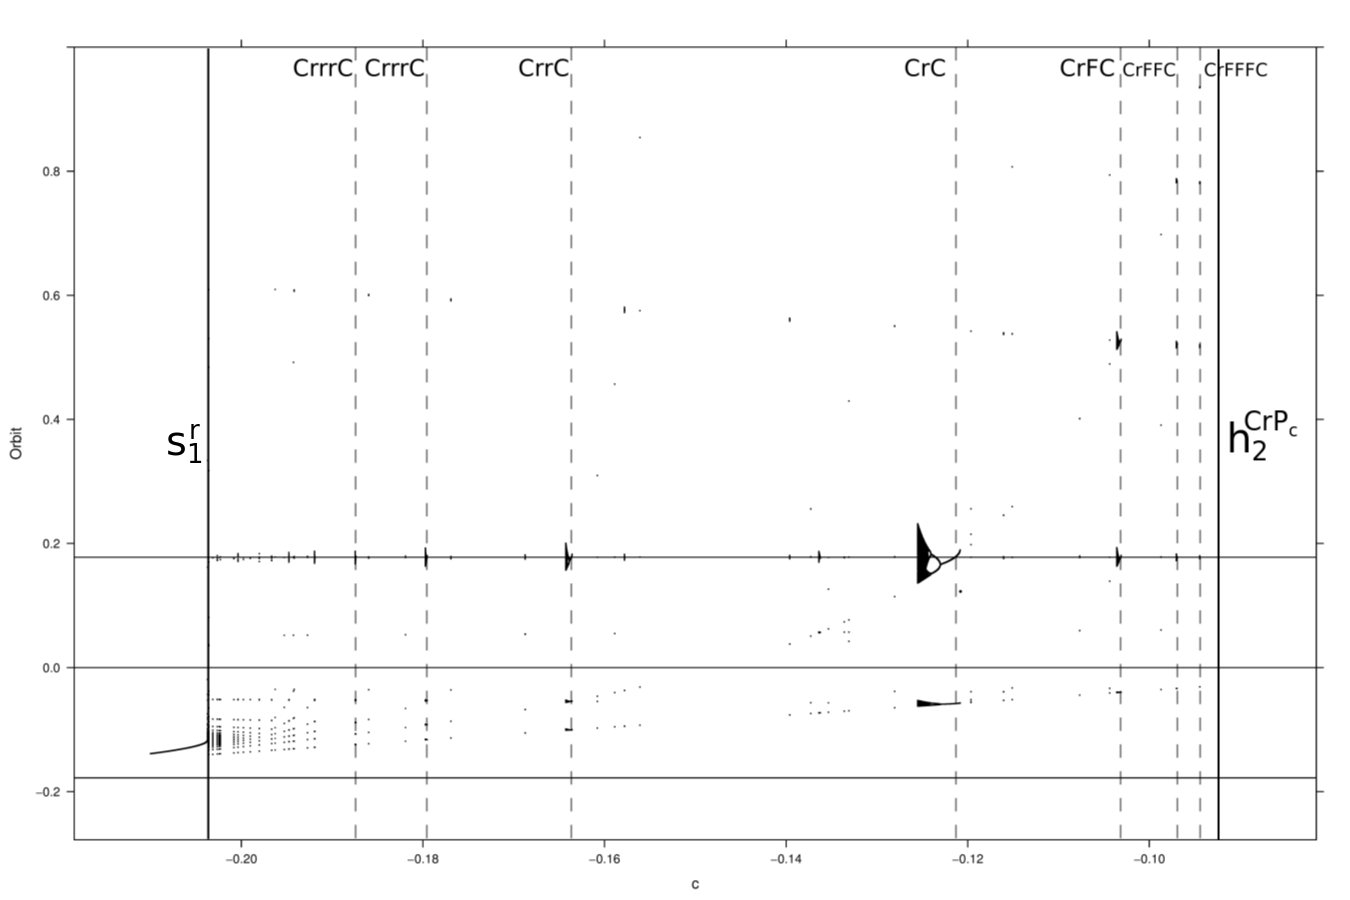
\includegraphics[width=.8\textwidth]{./img/over.png}
		\caption{Orbit Diagram for $x^2 + c + \frac{.001}{x^2}$}
	\end{figure}
\end{frame}

\begin{frame}[allowframebreaks]{Graphical Iteration}
\begin{figure}[ht]
		\centering
		% \begin{subfigure}[b]{.49\textwidth}
		% 		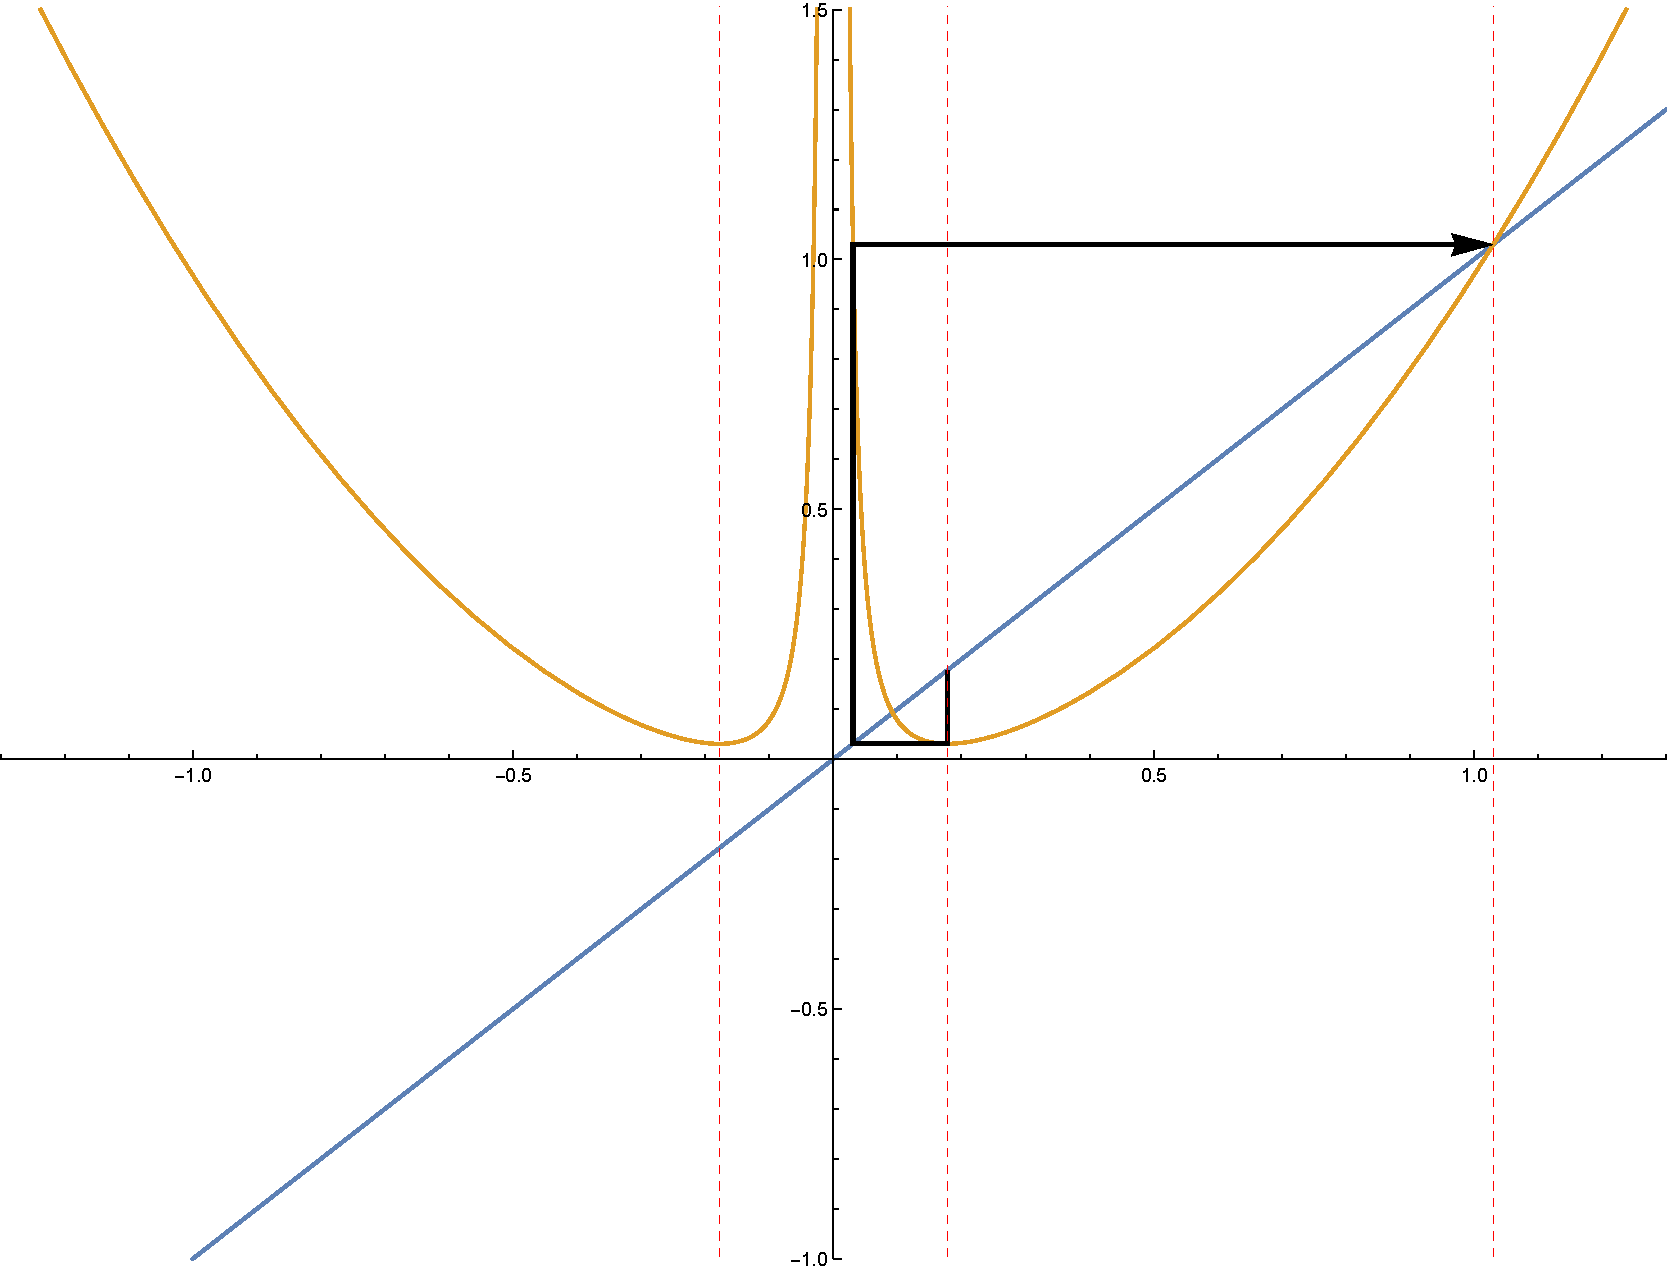
\includegraphics[width=\textwidth]{./img/plot-003255}
		% 		\caption{$c \approx h_2^{CLP_c}$}
		% \end{subfigure}
		% \begin{subfigure}[b]{.49\textwidth}
		% 		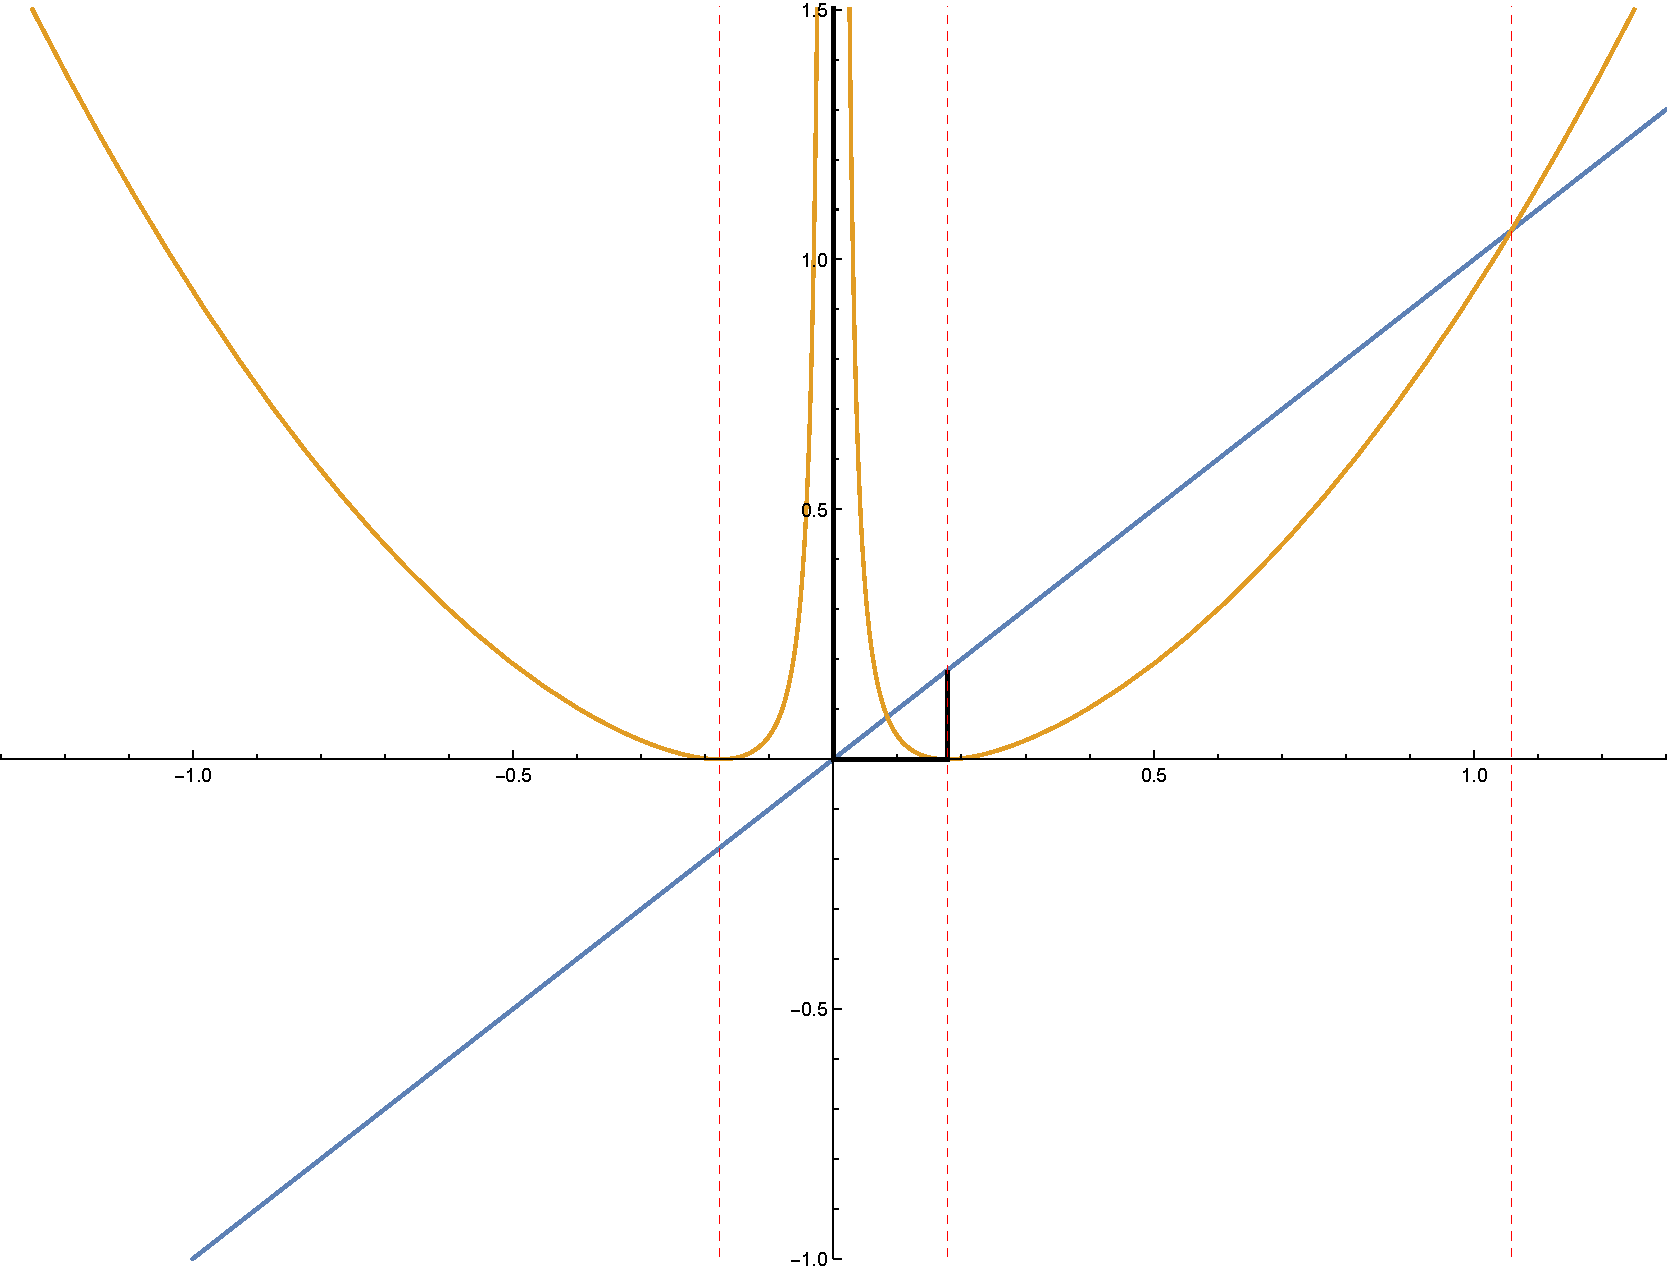
\includegraphics[width=\textwidth]{./img/plot-006355}
		% 		\caption{$c \approx z_1^{C0}$}
		% \end{subfigure}

		\begin{subfigure}[b]{.49\textwidth}
				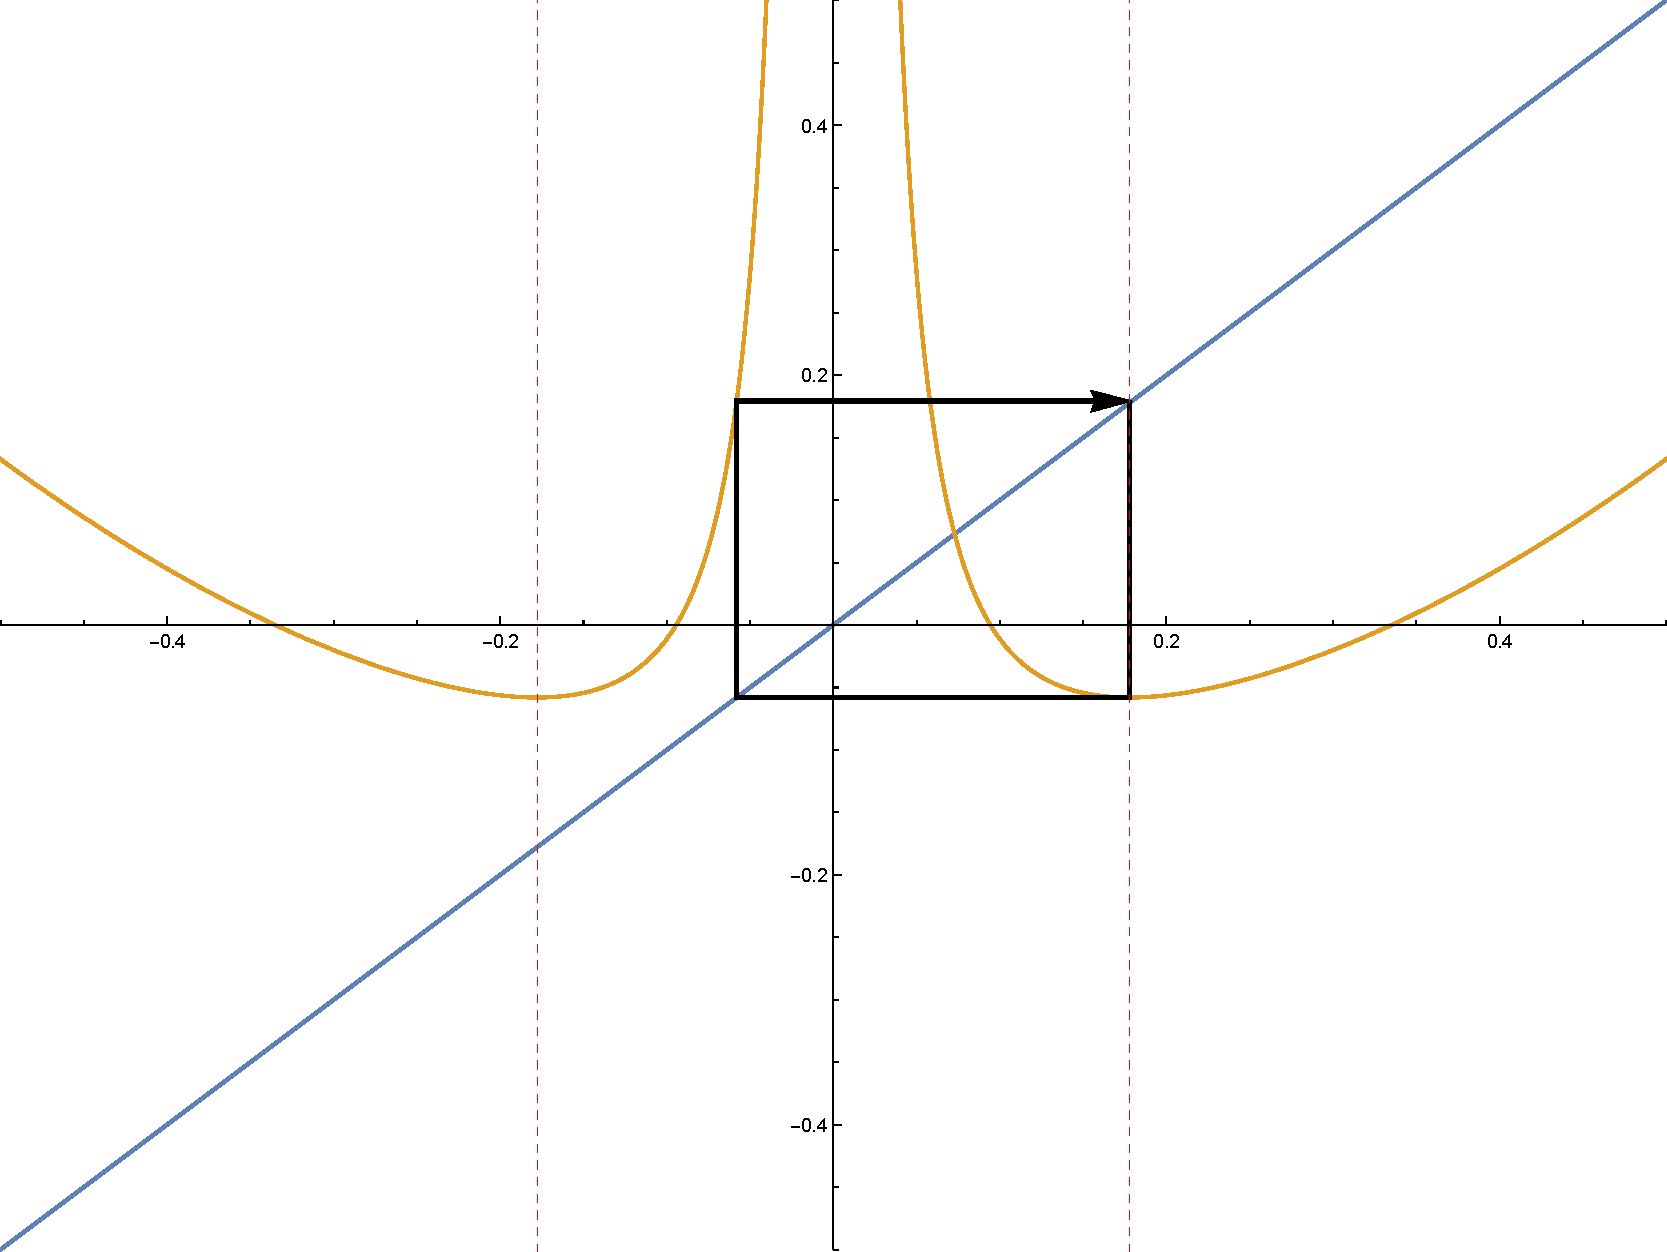
\includegraphics[width=\textwidth]{./img/plot-012125}
				\caption{$c \approx - .12125 \approx p_2^{Cr}$}
		\end{subfigure}
		\begin{subfigure}[b]{.49\textwidth}
				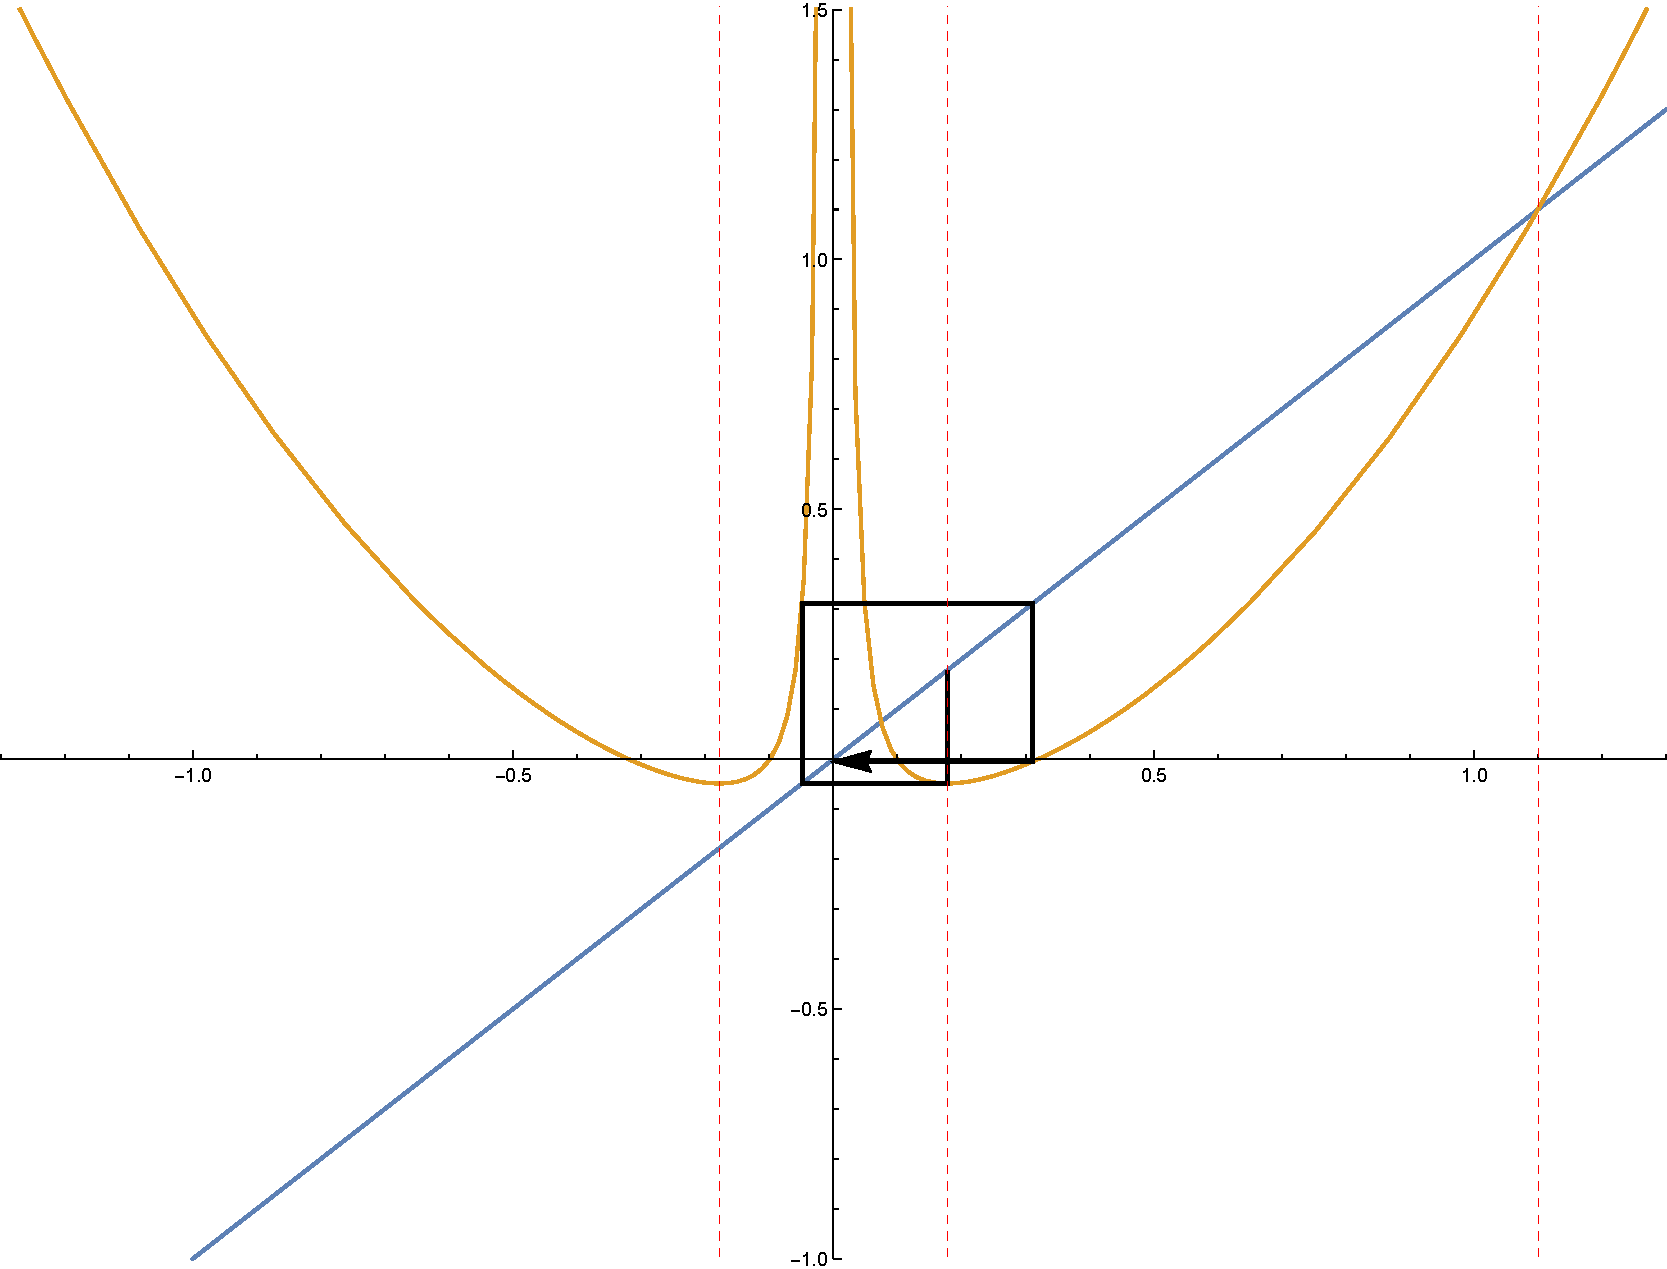
\includegraphics[width=\textwidth]{./img/plot-0112}
				\caption{$c \approx -.112 \approx z_3^{CrF0}$}
		\end{subfigure}

		\begin{subfigure}[b]{.49\textwidth}
				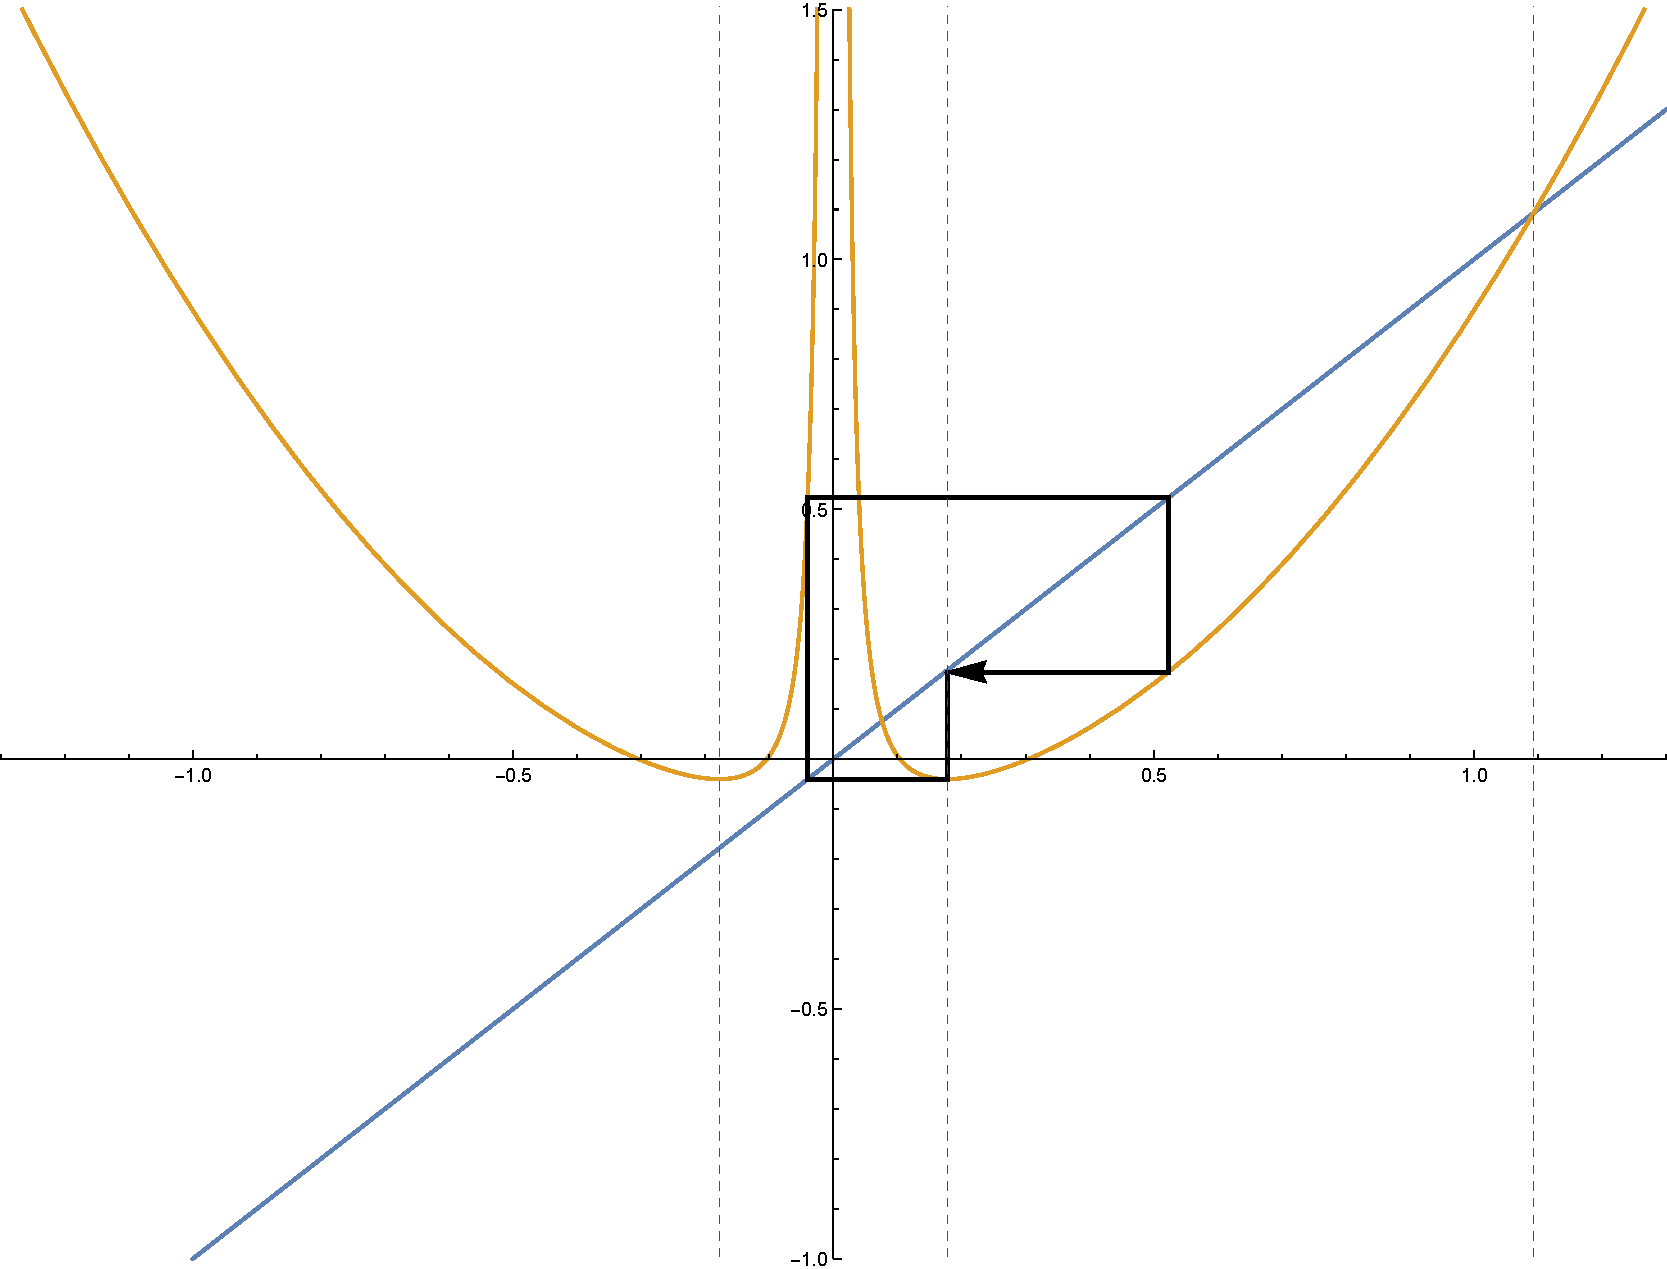
\includegraphics[width=\textwidth]{./img/plot-010325}
				\caption{$c \approx - .10325 \approx p_3^{CrF}$}
		\end{subfigure}
		\begin{subfigure}[b]{.49\textwidth}
				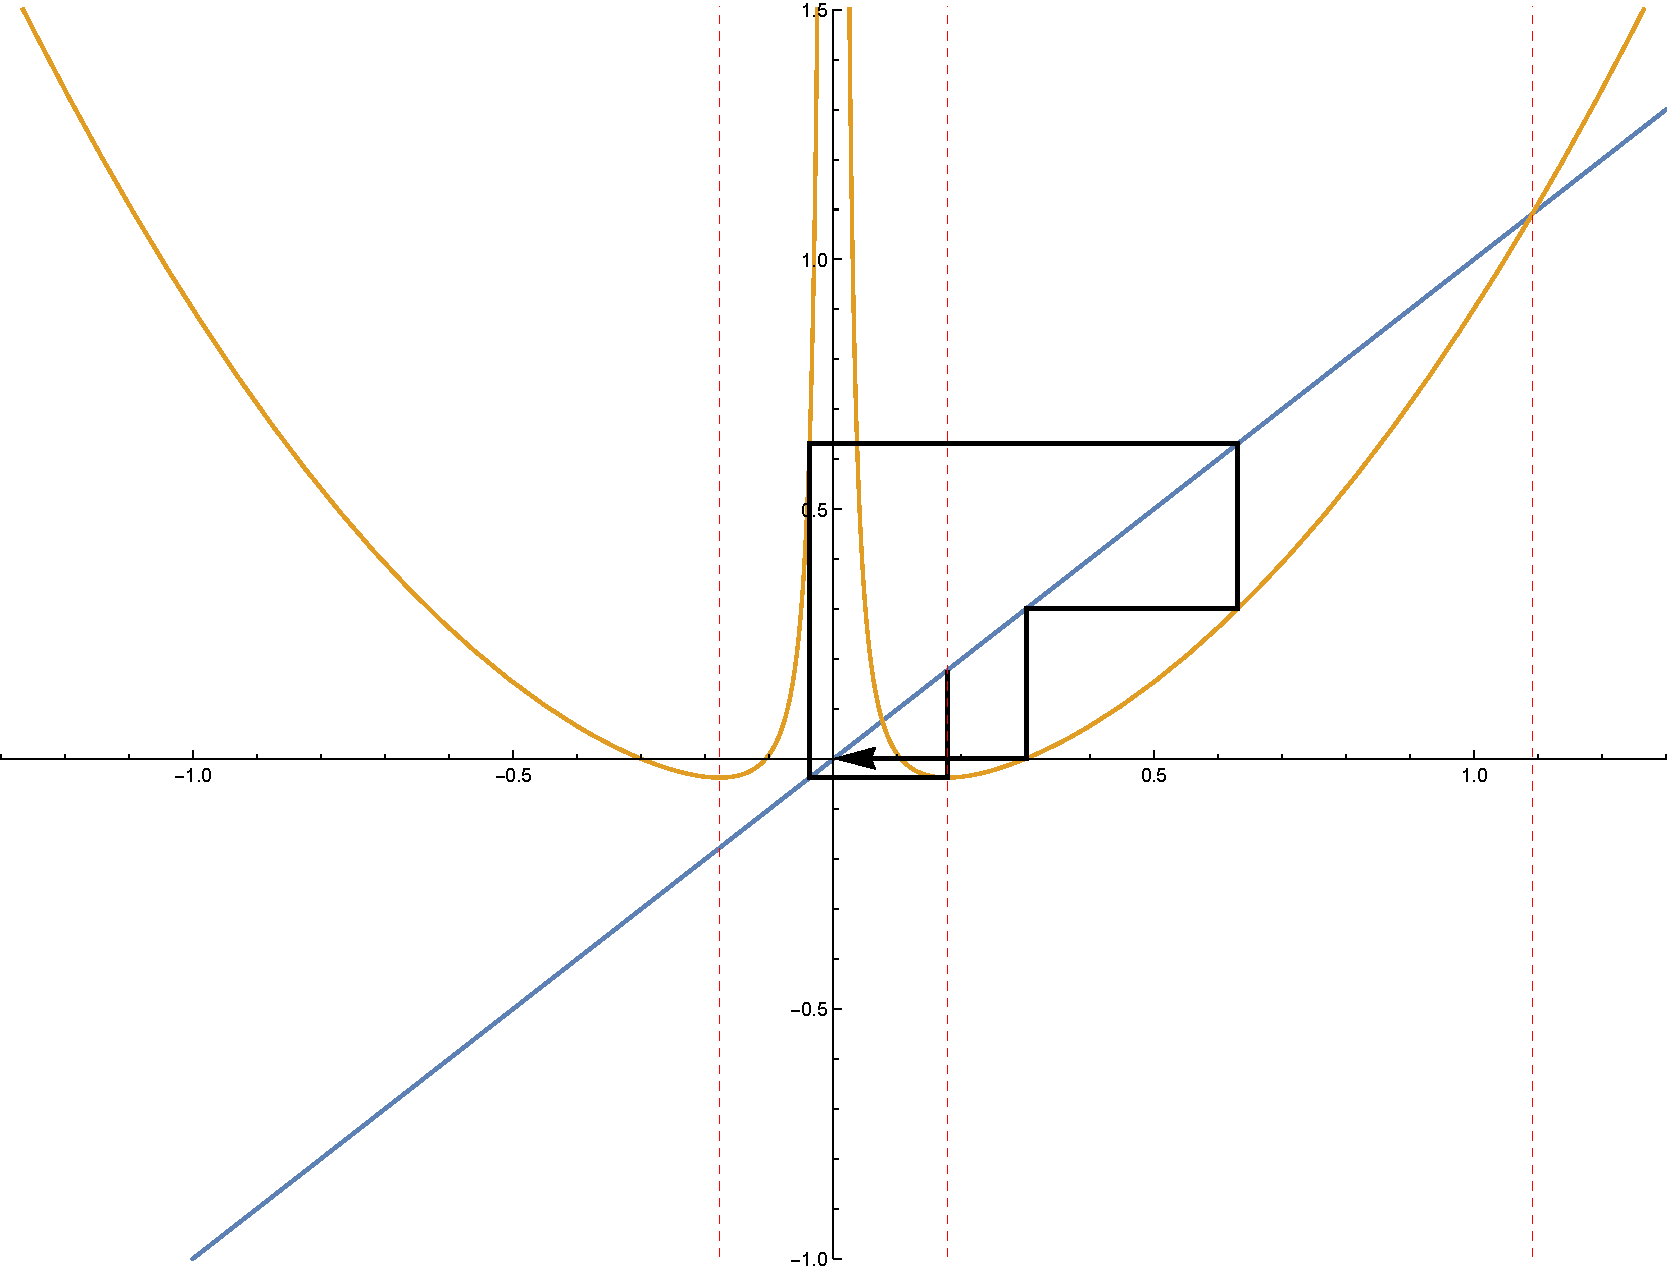
\includegraphics[width=\textwidth]{./img/plot-010025}
				\caption{$c \approx -.10025 \approx z_4^{CrFF0}$}
		\end{subfigure}
		
		\begin{subfigure}[b]{.49\textwidth}
				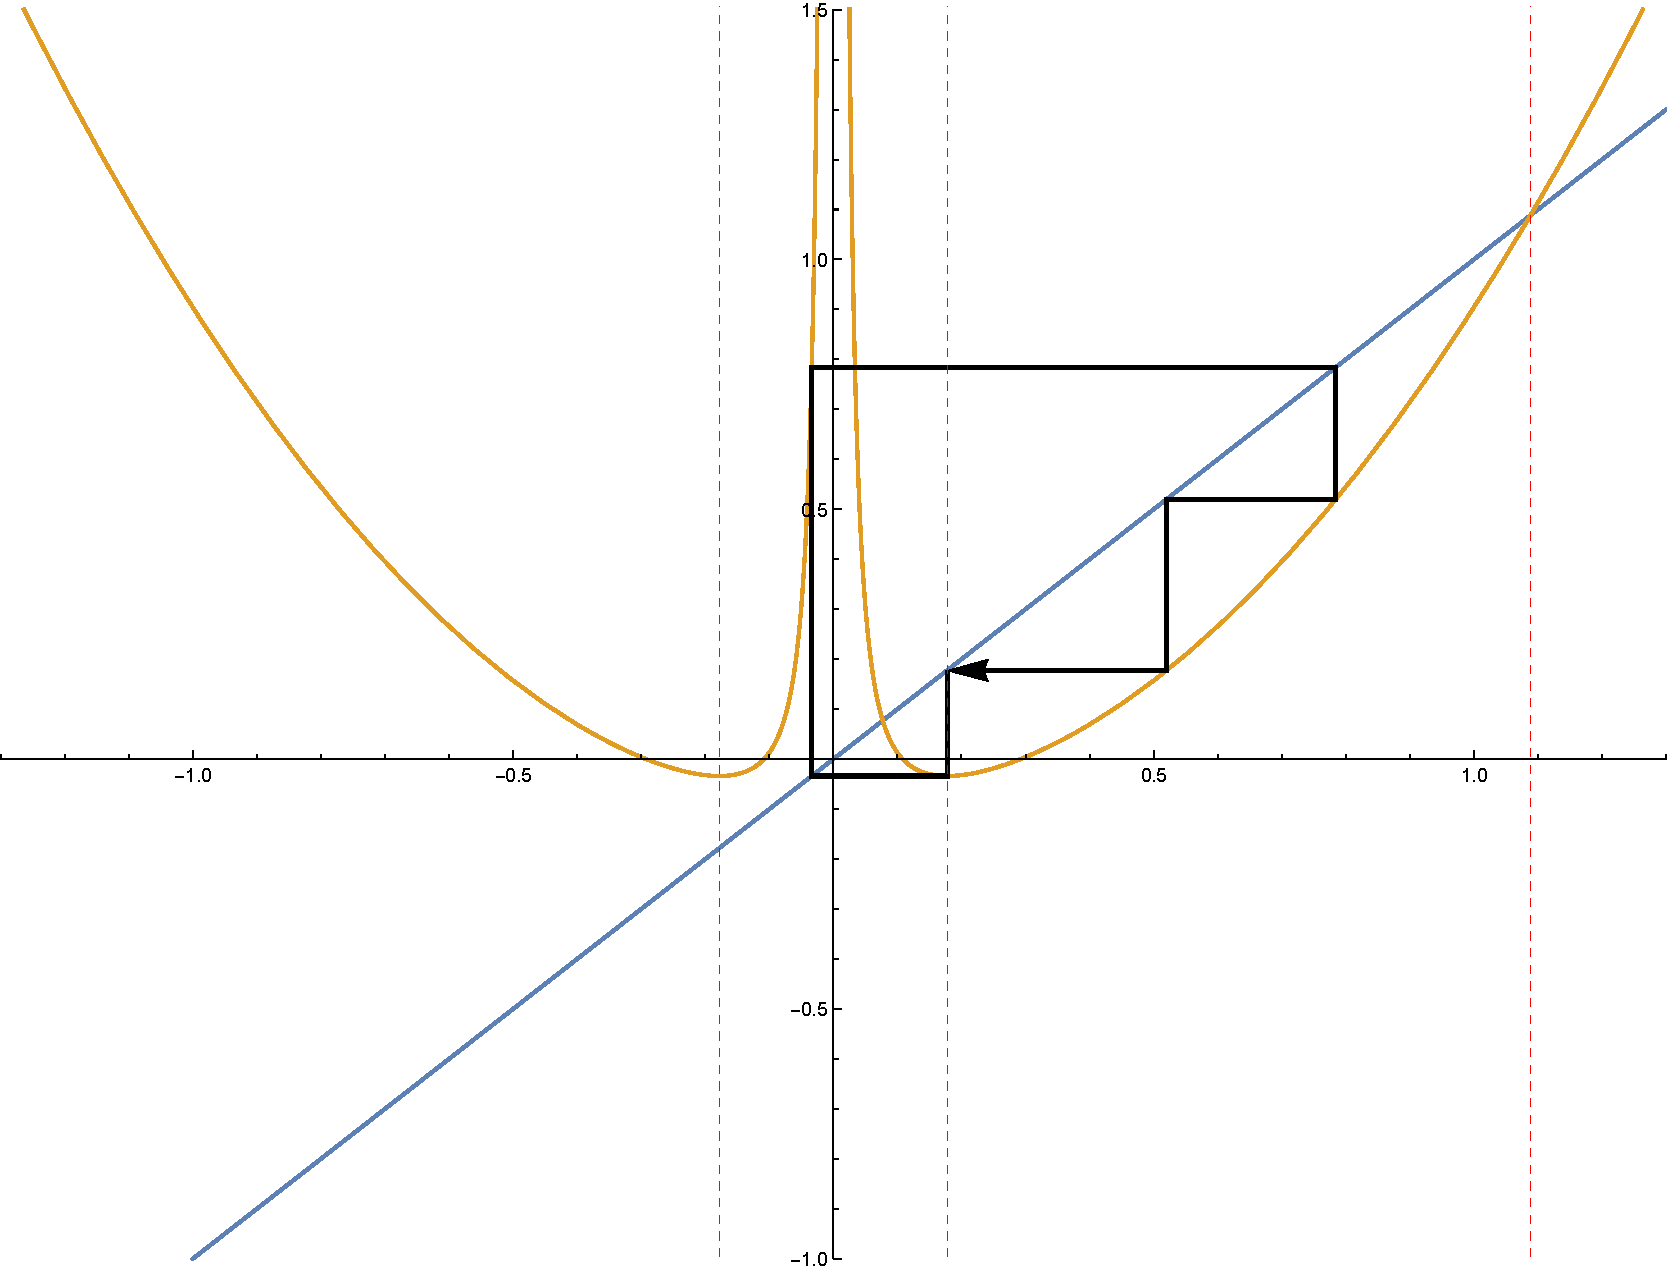
\includegraphics[width=\textwidth]{./img/plot-009695}
				\caption{$c \approx -.09695 \approx p_4^{CrFF}$}
		\end{subfigure}
		\begin{subfigure}[b]{.49\textwidth}
				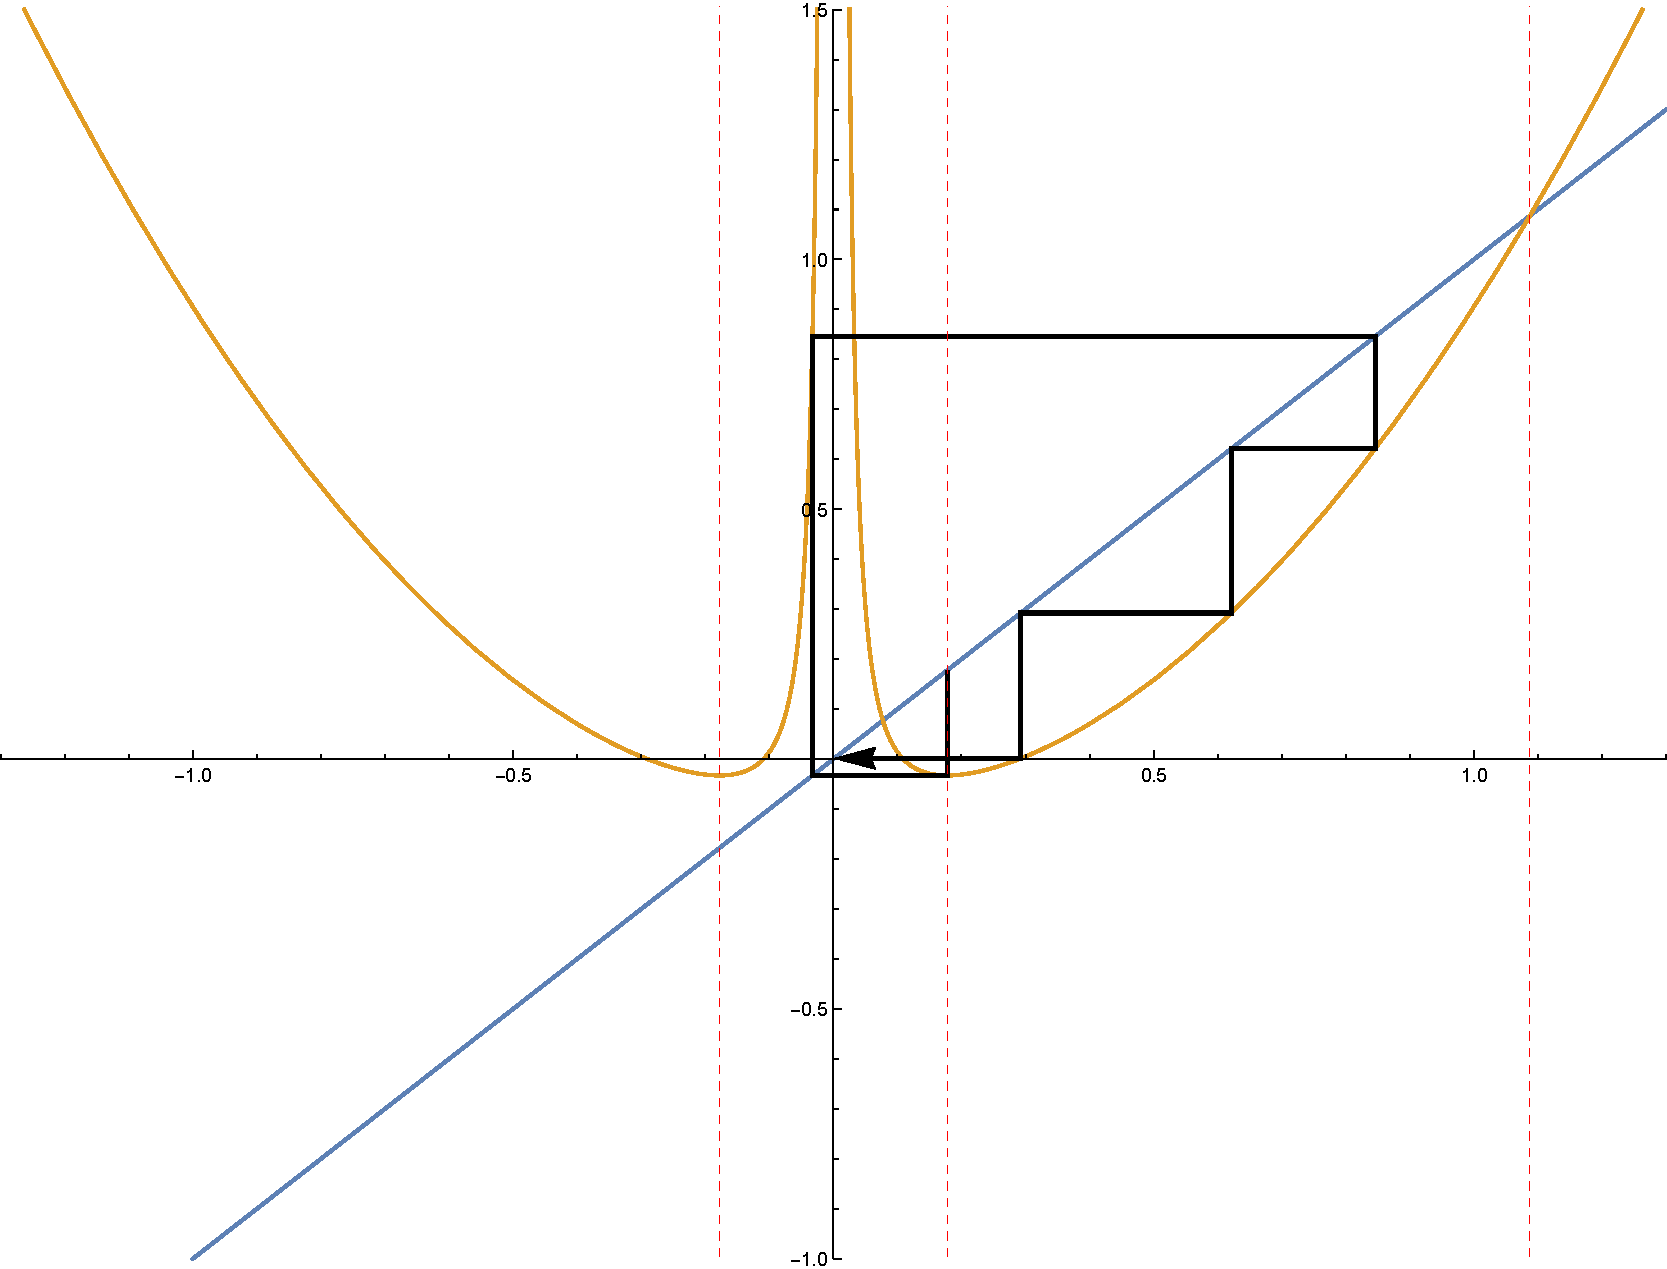
\includegraphics[width=\textwidth]{./img/plot-009585}
				\caption{$c \approx -.09585 \approx z_5^{CrFFF0}$}
		\end{subfigure}


		\begin{subfigure}[b]{.49\textwidth}
				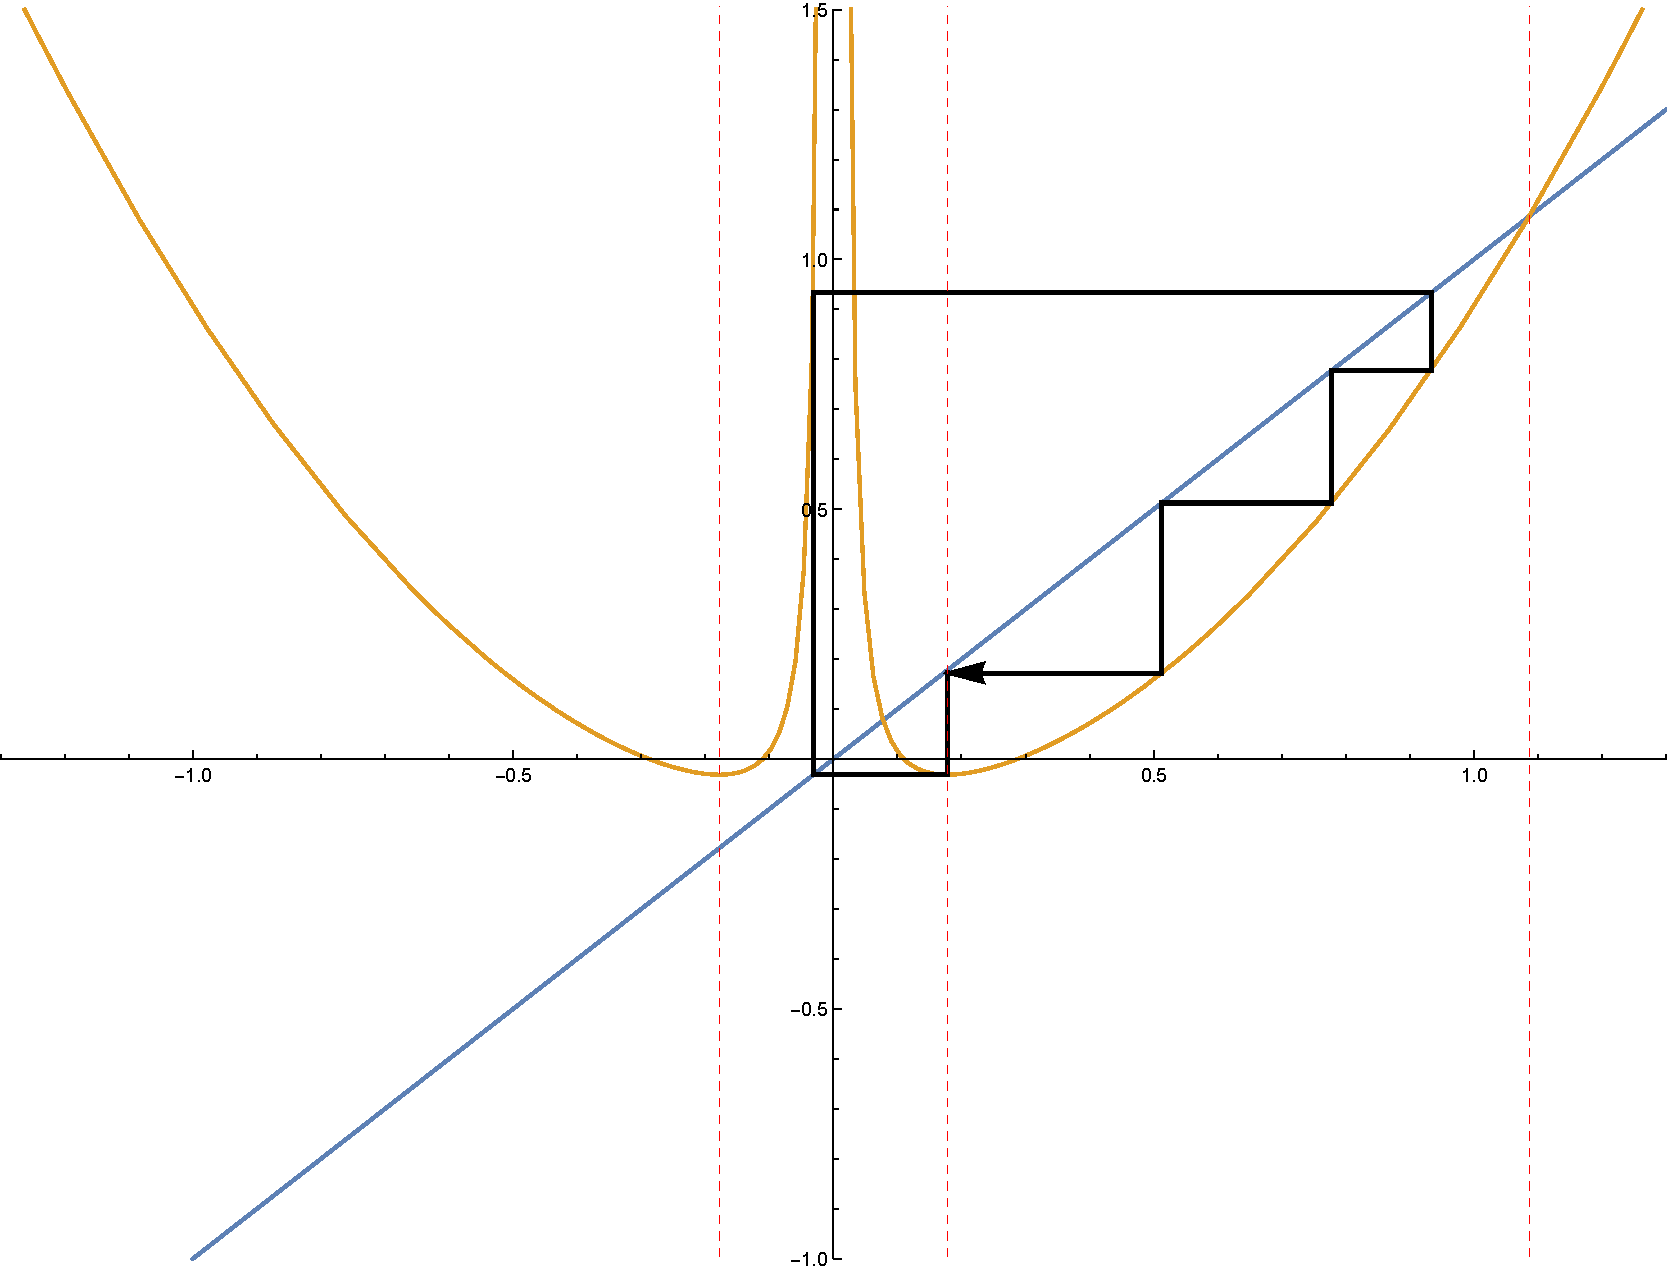
\includegraphics[width=\textwidth]{./img/plot-009445}
				\caption{$c \approx p_5^{CrFFF}$}
		\end{subfigure}
		\begin{subfigure}[b]{.49\textwidth}
				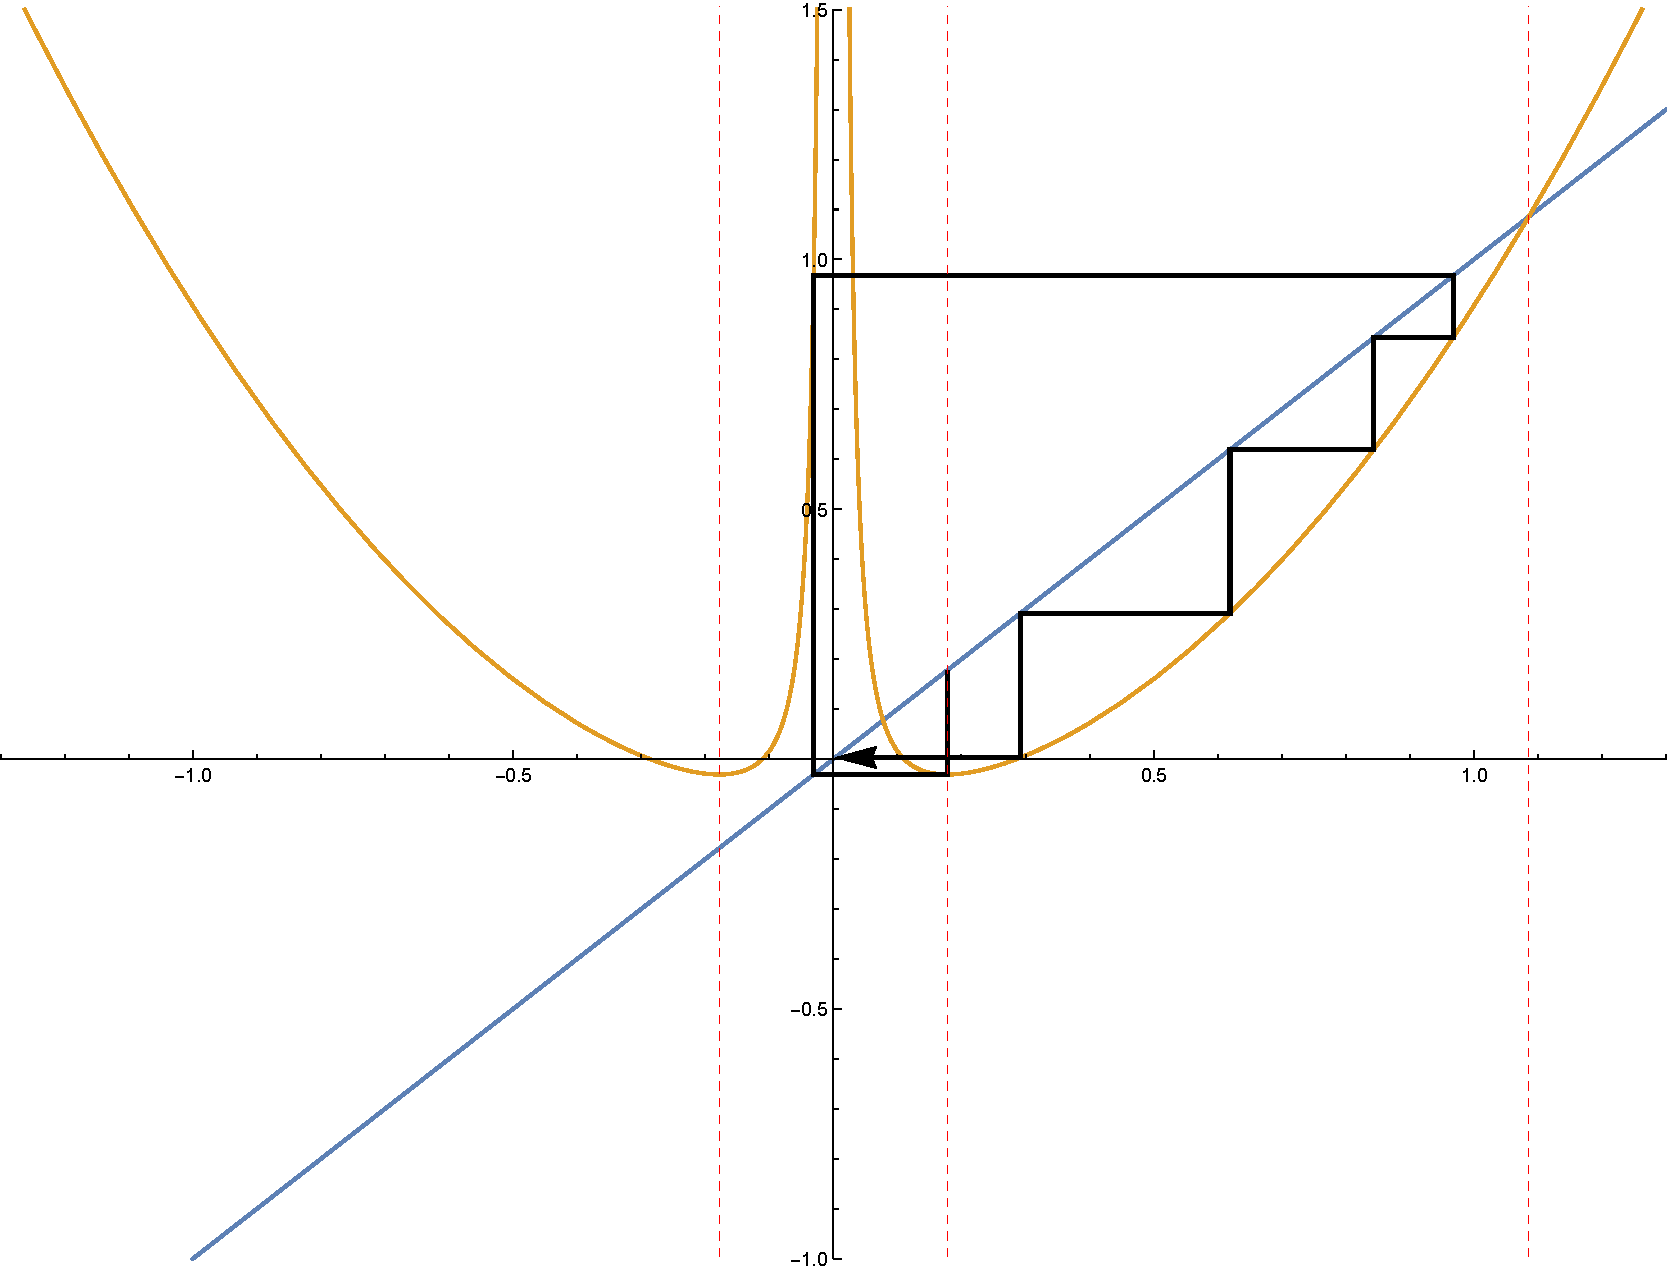
\includegraphics[width=\textwidth]{./img/plot-009395}
				\caption{$c \approx z_6^{CrFFFF0}$}
		\end{subfigure}
		
		\begin{subfigure}[b]{.49\textwidth}
				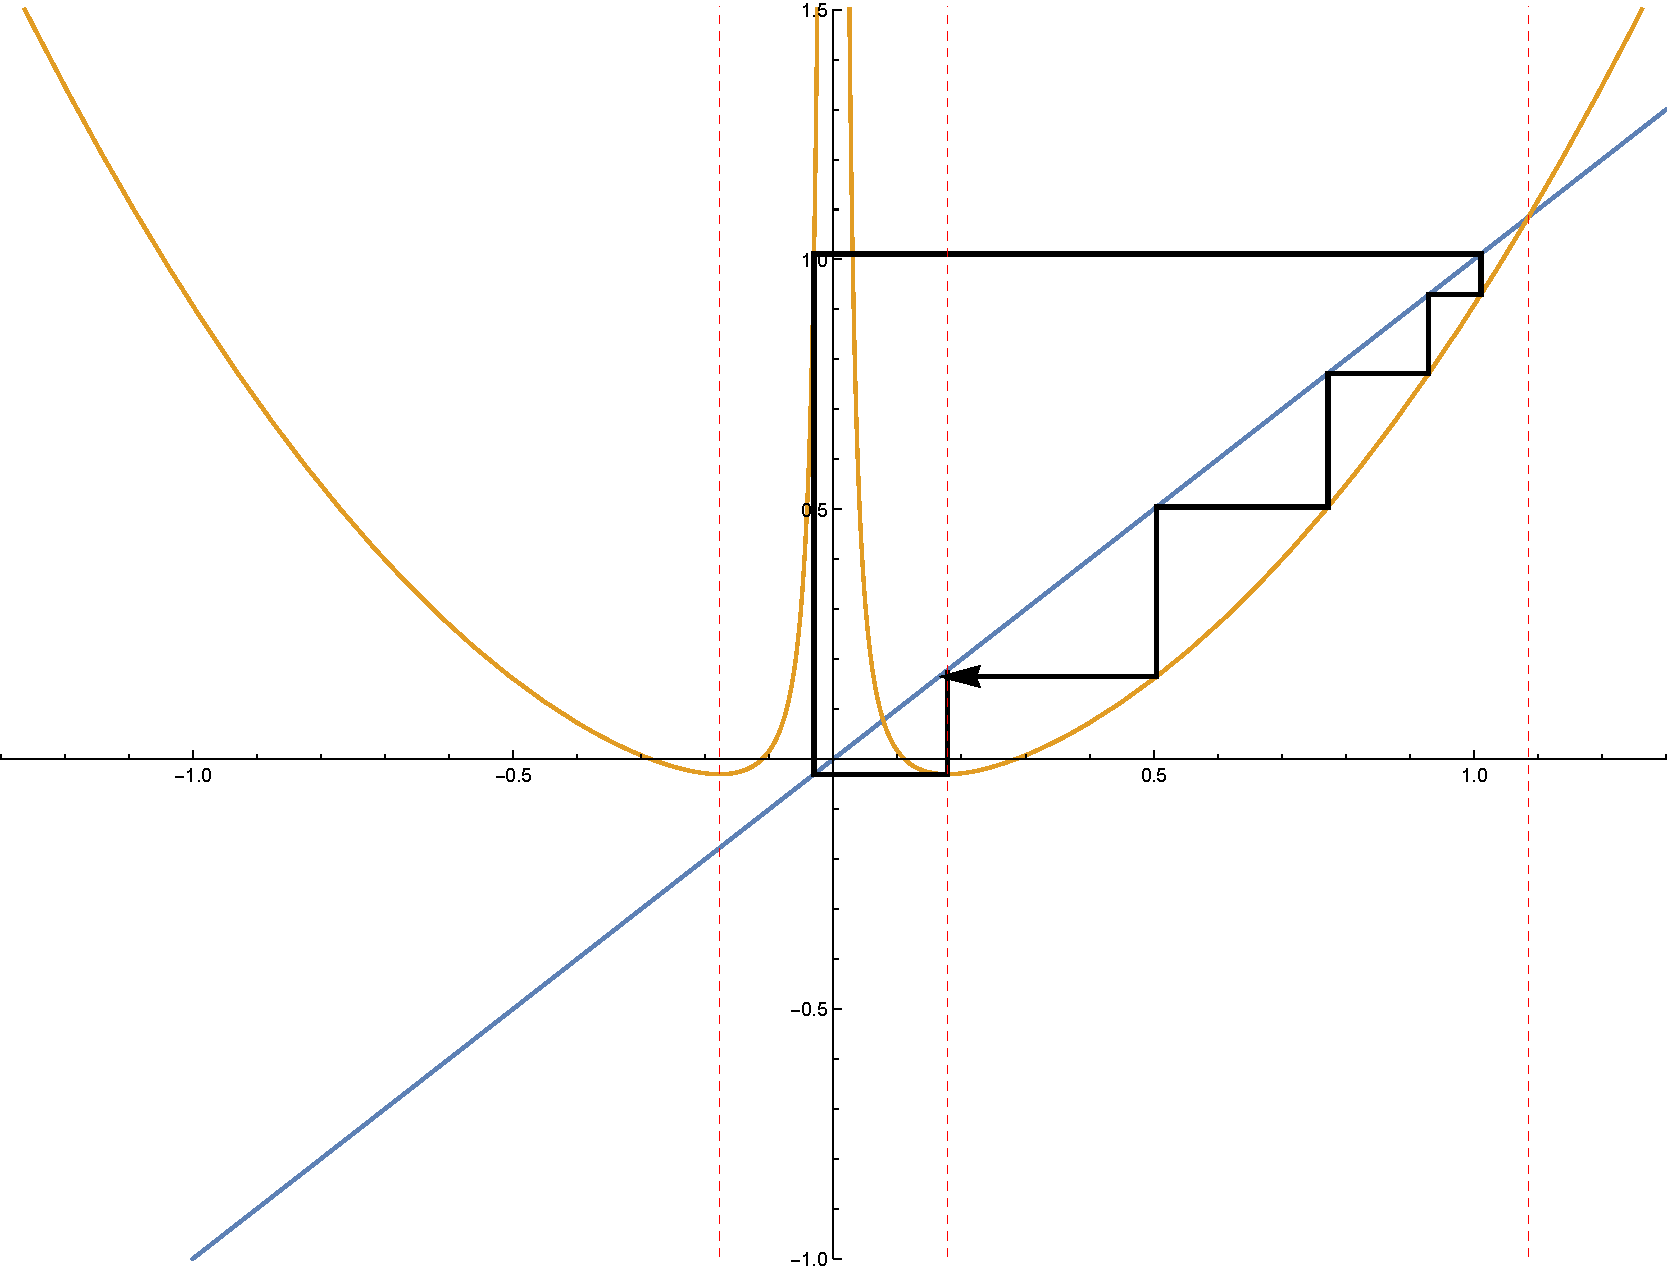
\includegraphics[width=\textwidth]{./img/plot-009335}
				\caption{$c \approx p_6^{CrFFFF}$}
		\end{subfigure}
		\begin{subfigure}[b]{.49\textwidth}
				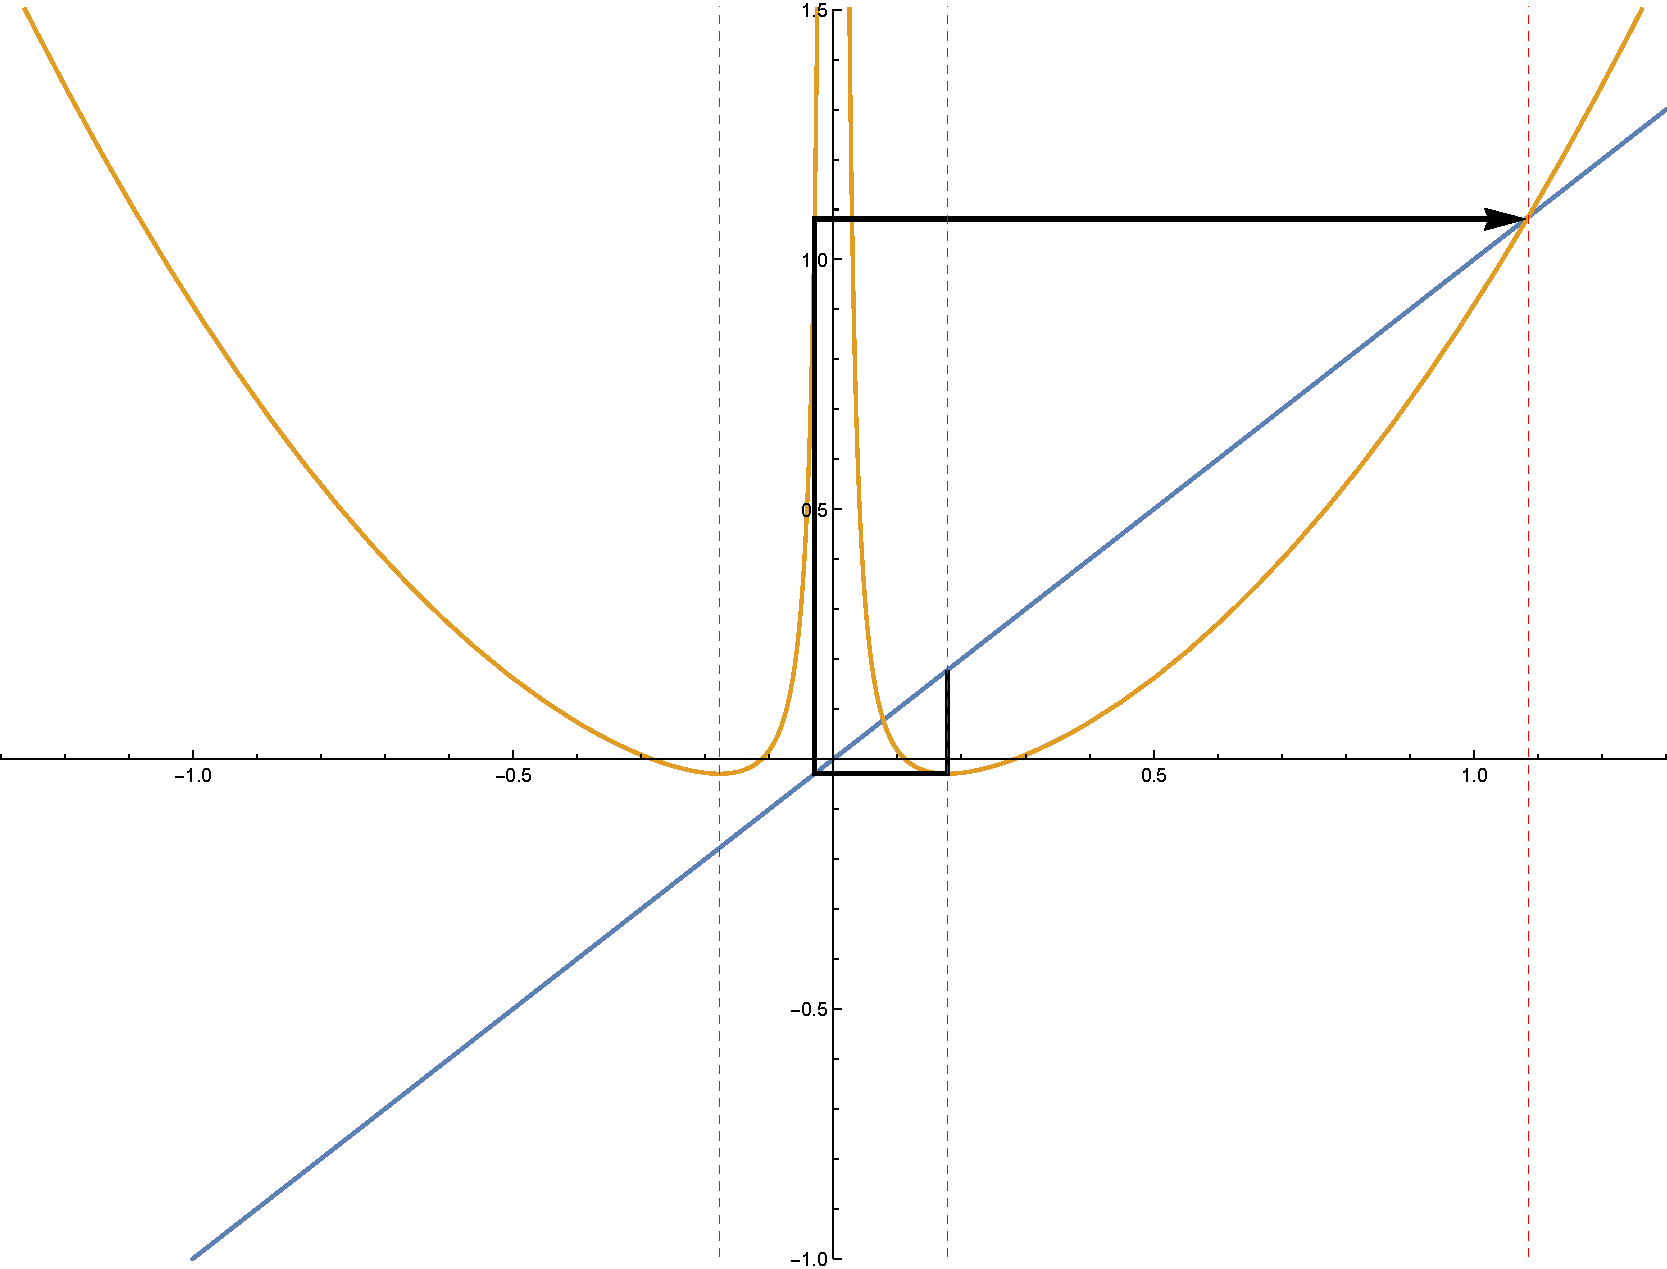
\includegraphics[width=\textwidth]{./img/plot-009245}
				\caption{$c \approx h_2^{CrP_c}$}
		\end{subfigure}
		% \begin{subfigure}[b]{.4\textwidth}
		% 		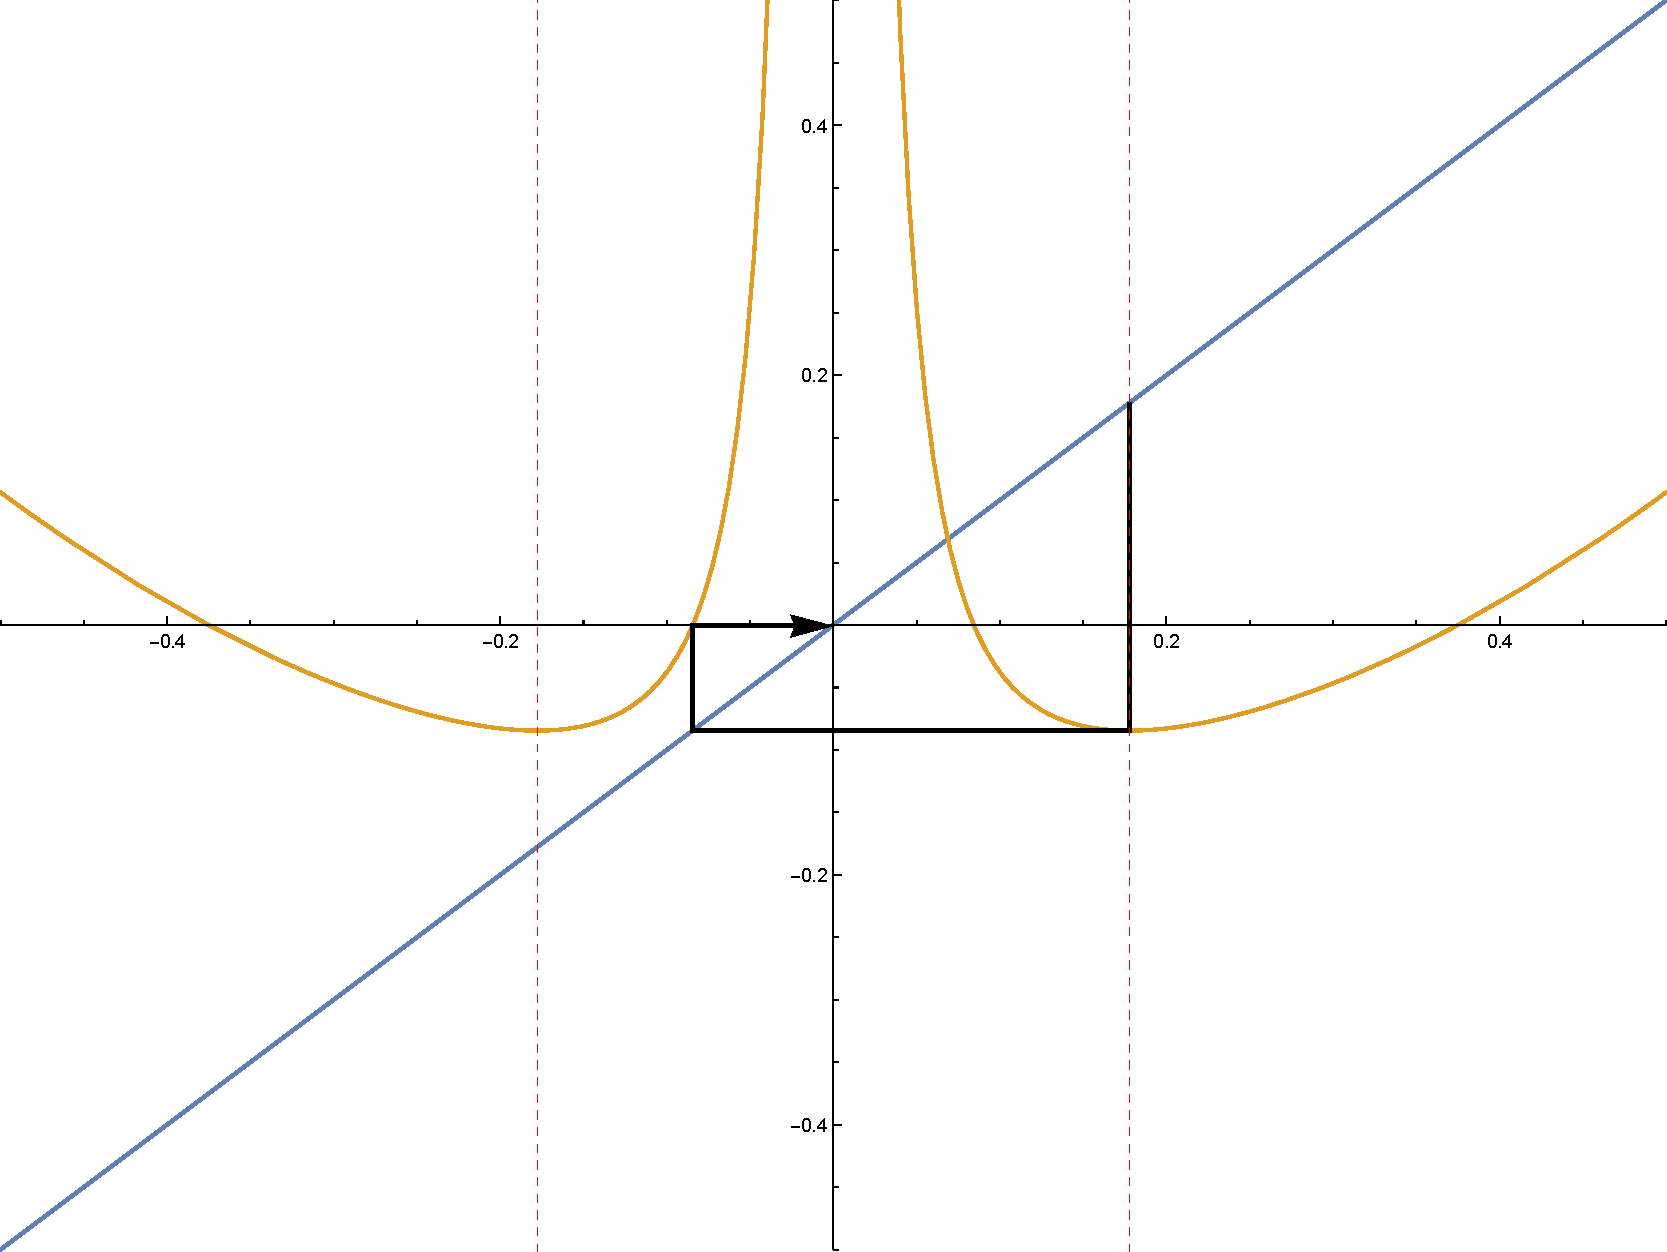
\includegraphics[width=\textwidth]{./img/plot-014778}
		% 		\caption{$c \approx -.14778 \approx z_2^{Cr0}$}
		% \end{subfigure}
		% \begin{subfigure}[b]{0.3\textwidth}
		% 		\includegraphics[width=\textwidth]{./img/plot-}
		% 		\caption{Seventh iterate of $f_c (C)$ added along with the parameter value of its prezero orbit}
		% 		\label{fig:cplot6S}
		% \end{subfigure}
		% \begin{subfigure}[b]{0.333\textwidth}
		% 		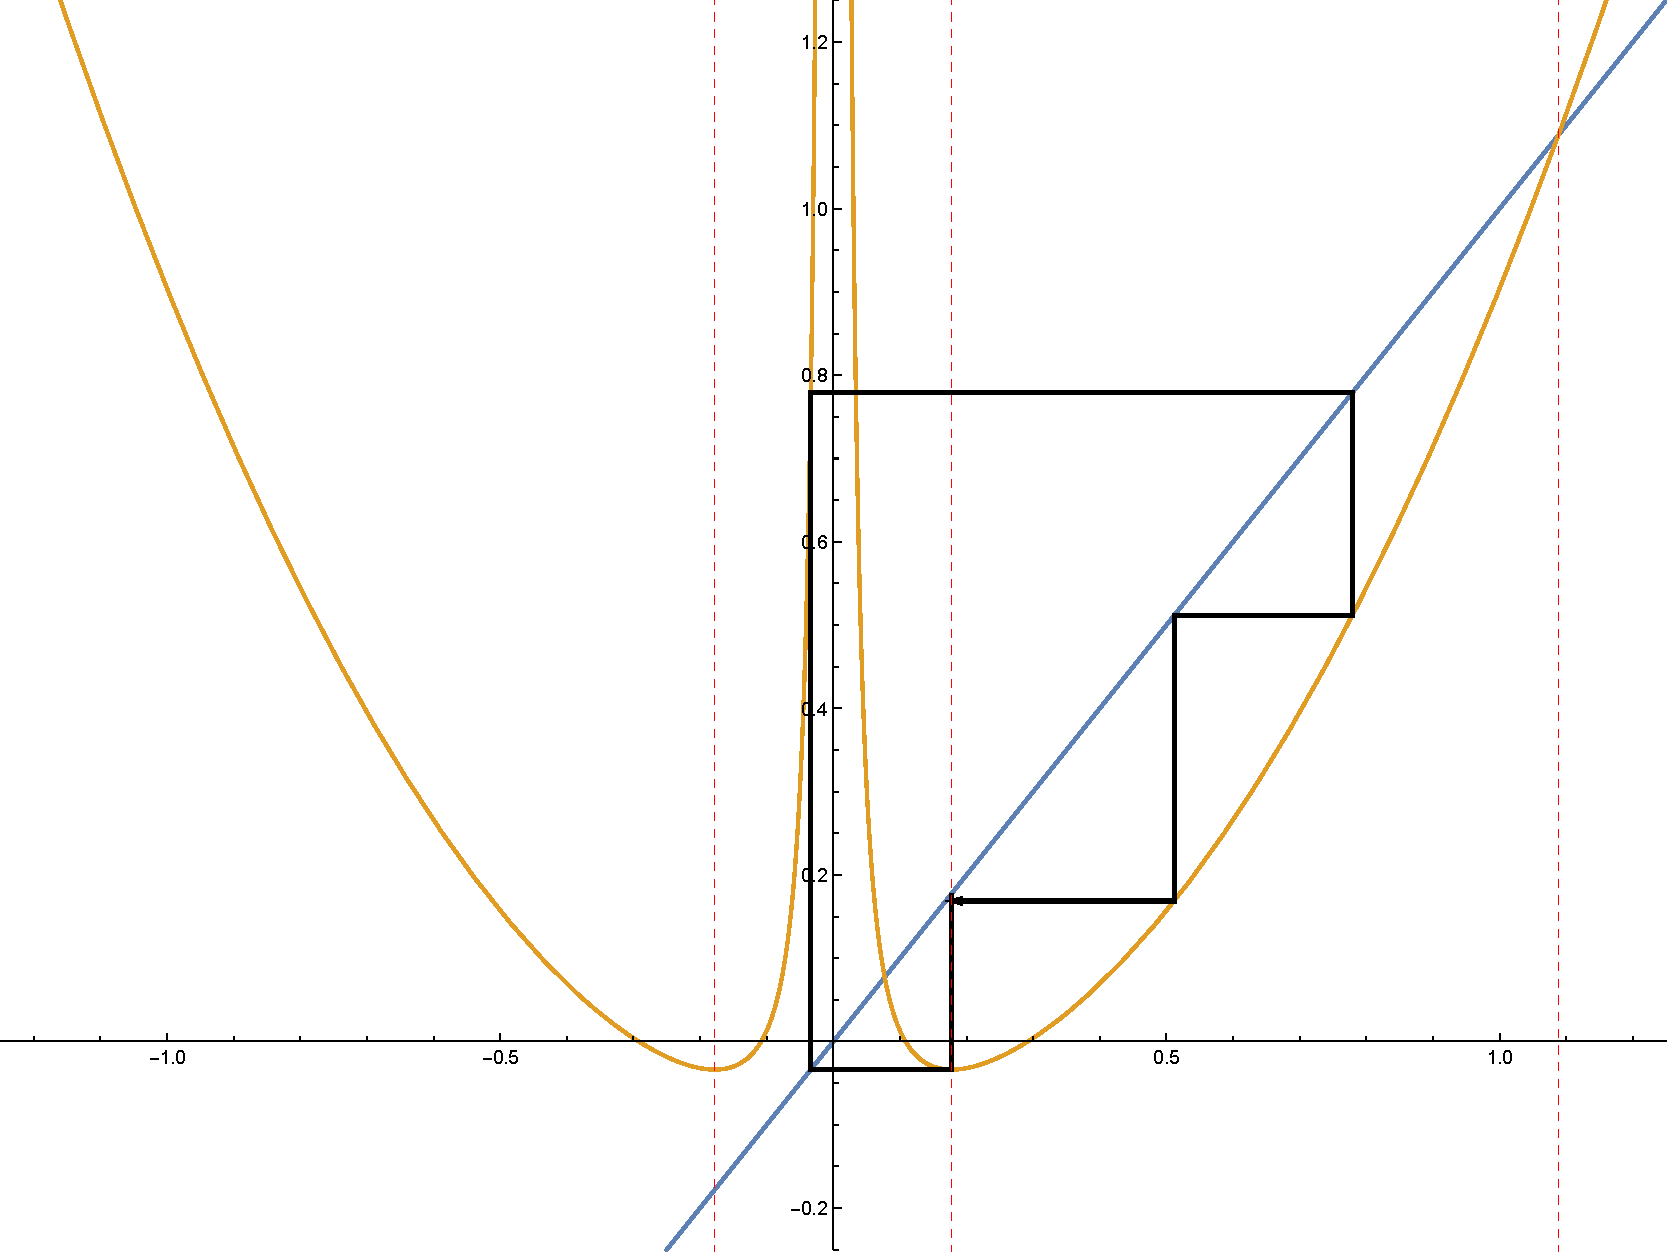
\includegraphics[width=\textwidth]{./img/CrFFC}
		% 		\caption{Seventh iterate of $f_c (C)$ added along with the parameter value of its prezero orbit}
		% 		\label{fig:cplot6S}
		% \end{subfigure}
		 %add desired spacing between images, e. g. ~, \quad, \qquad, \hfill etc.
		  % (or a blank line to force the subfigure onto a new line)
		%\caption{Graphical iteration showing the accumulation of periodic, prefixed, and prezero orbits as $c$ approaches $\pl$ (depicted in 3.10 (k)) from the right and the accumulation of periodic, and prezero orbits as $c$ approaches$\pr$ (depicted in 3.11 (k))  from the left}\label{fig:giters}
\end{figure}

\end{frame}

\begin{frame}[allowframebreaks]{Right Side Accumulation}
\begin{figure}[ht]
		\centering
		\begin{subfigure}[b]{0.5\textwidth}
				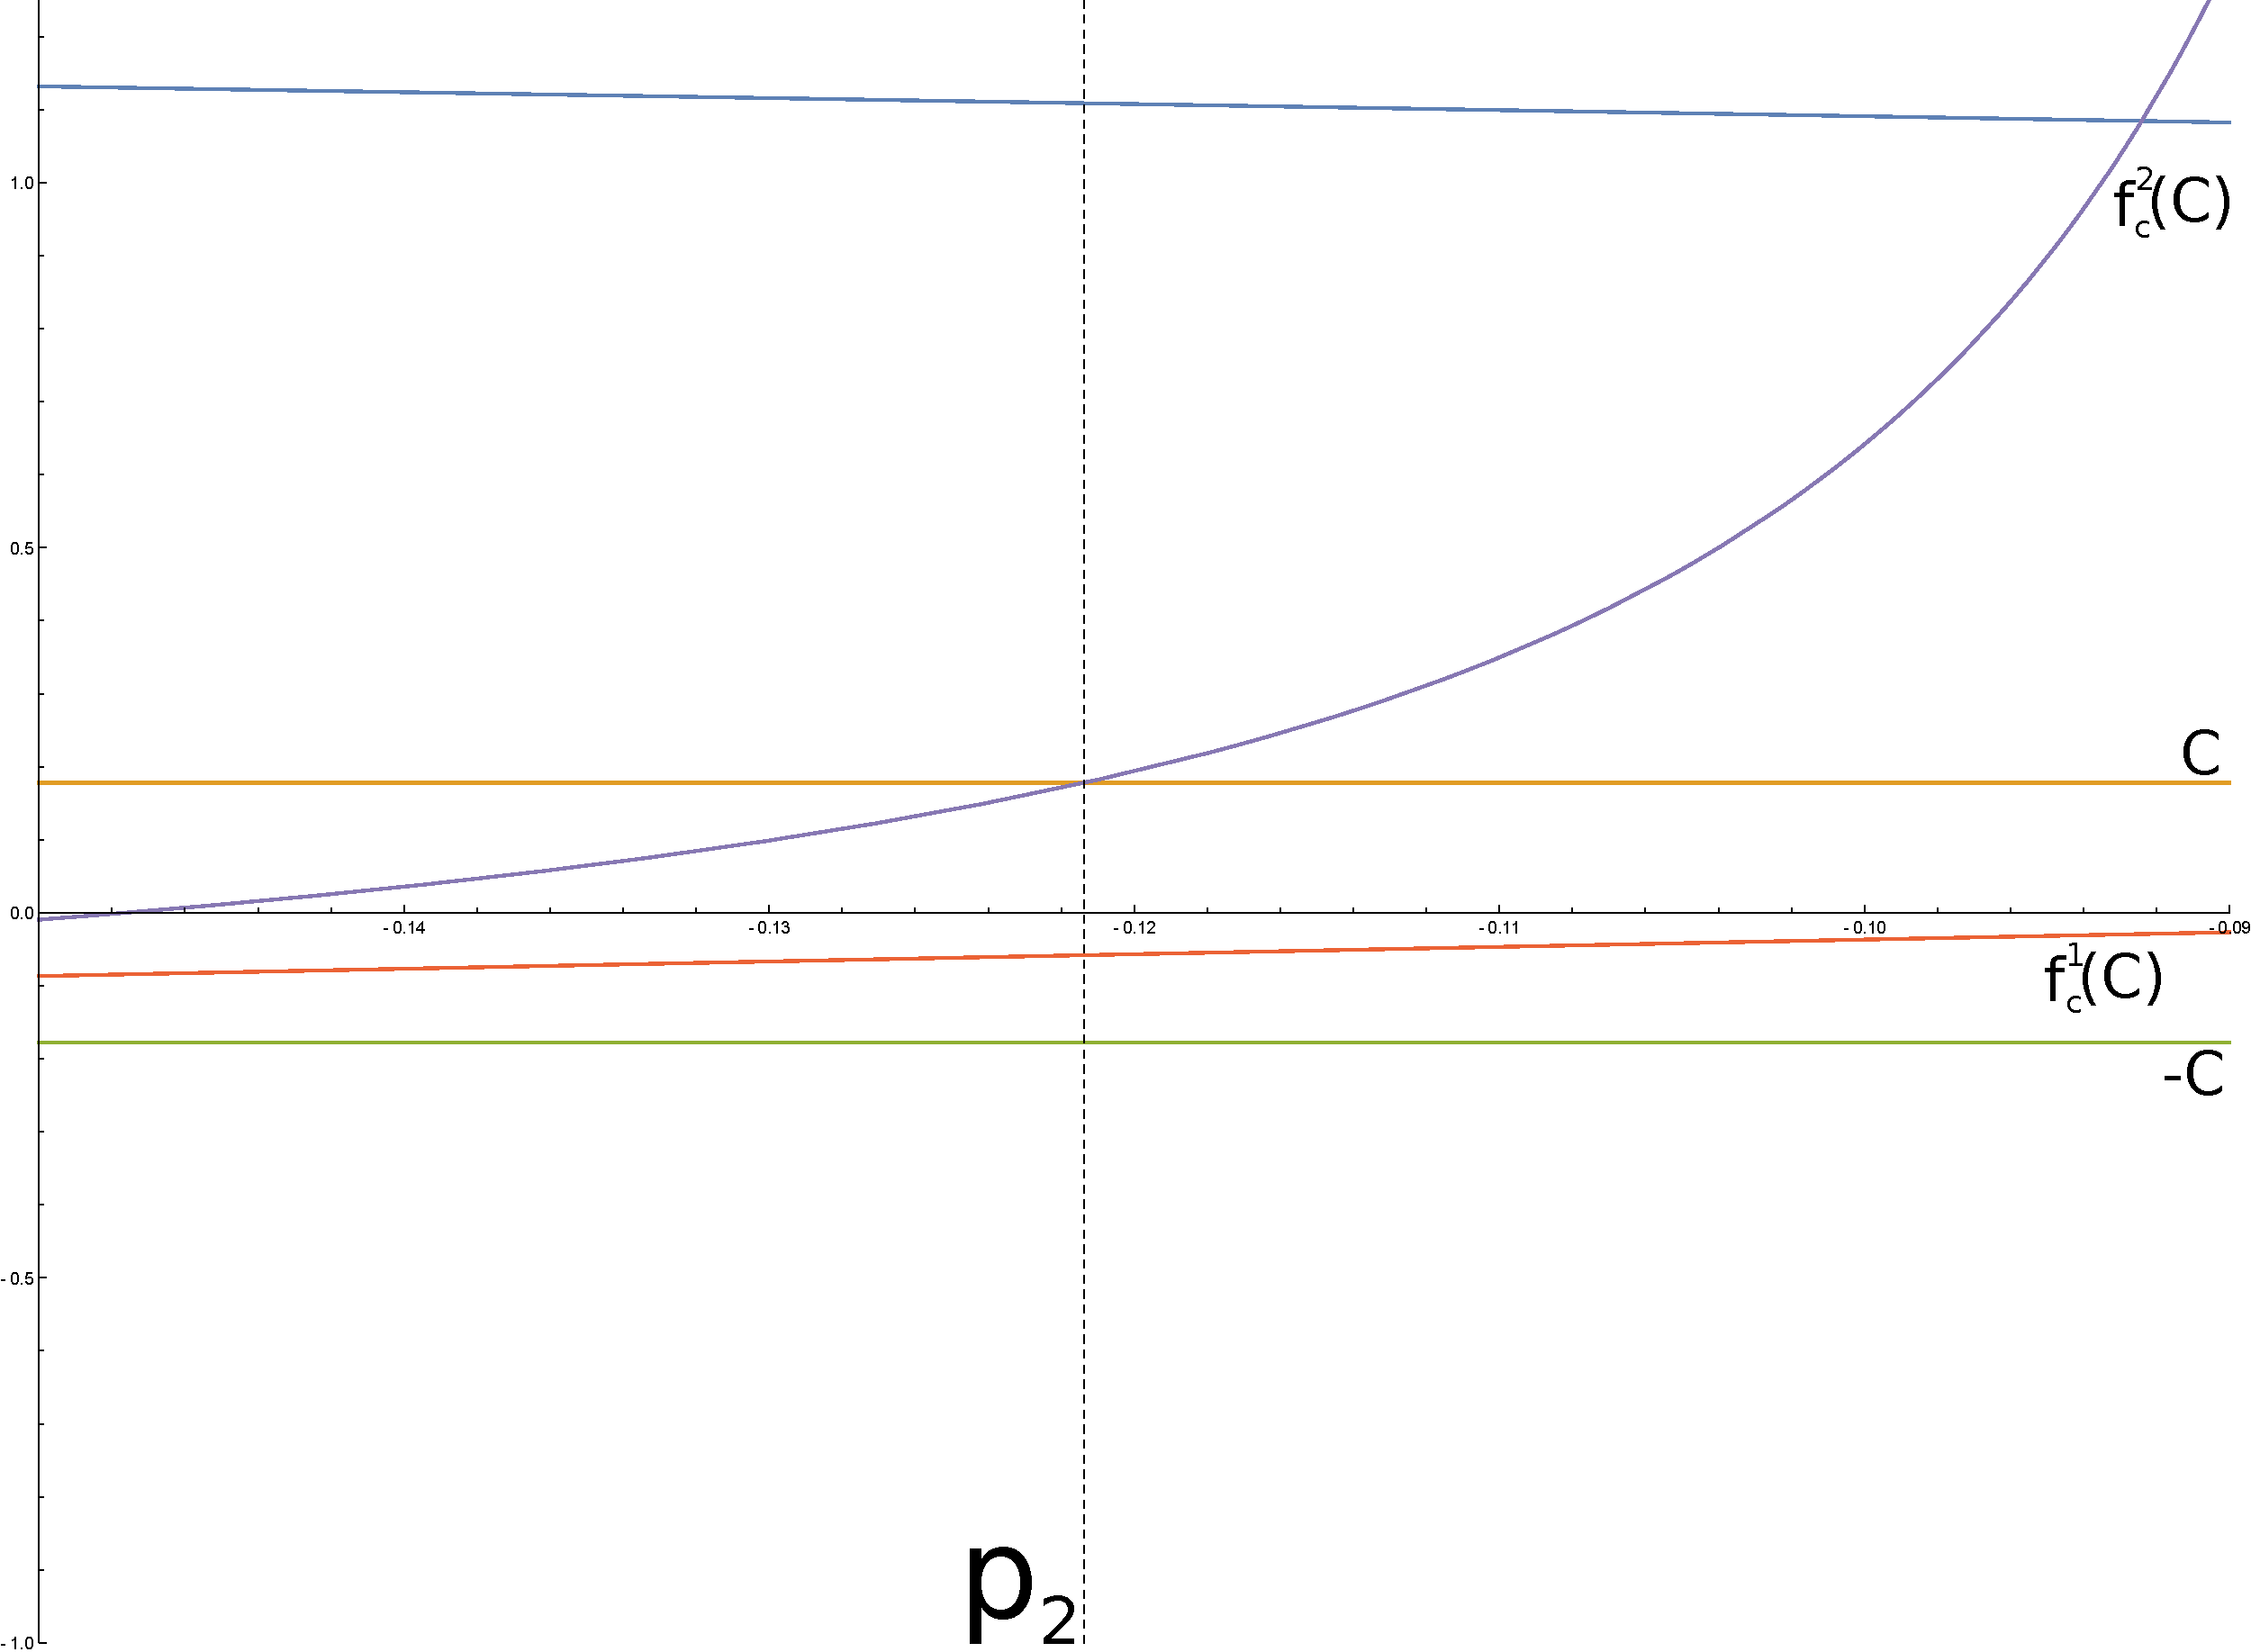
\includegraphics[width=\textwidth]{./img/cplot1H}
				\caption{$n = 2$}
				\label{fig:cplot1H}
		\end{subfigure}%
		~ %add desired spacing between images, e. g. ~, \quad, \qquad, \hfill etc.
		  % (or a blank line to force the subfigure onto a new line)
		\begin{subfigure}[b]{0.5\textwidth}
				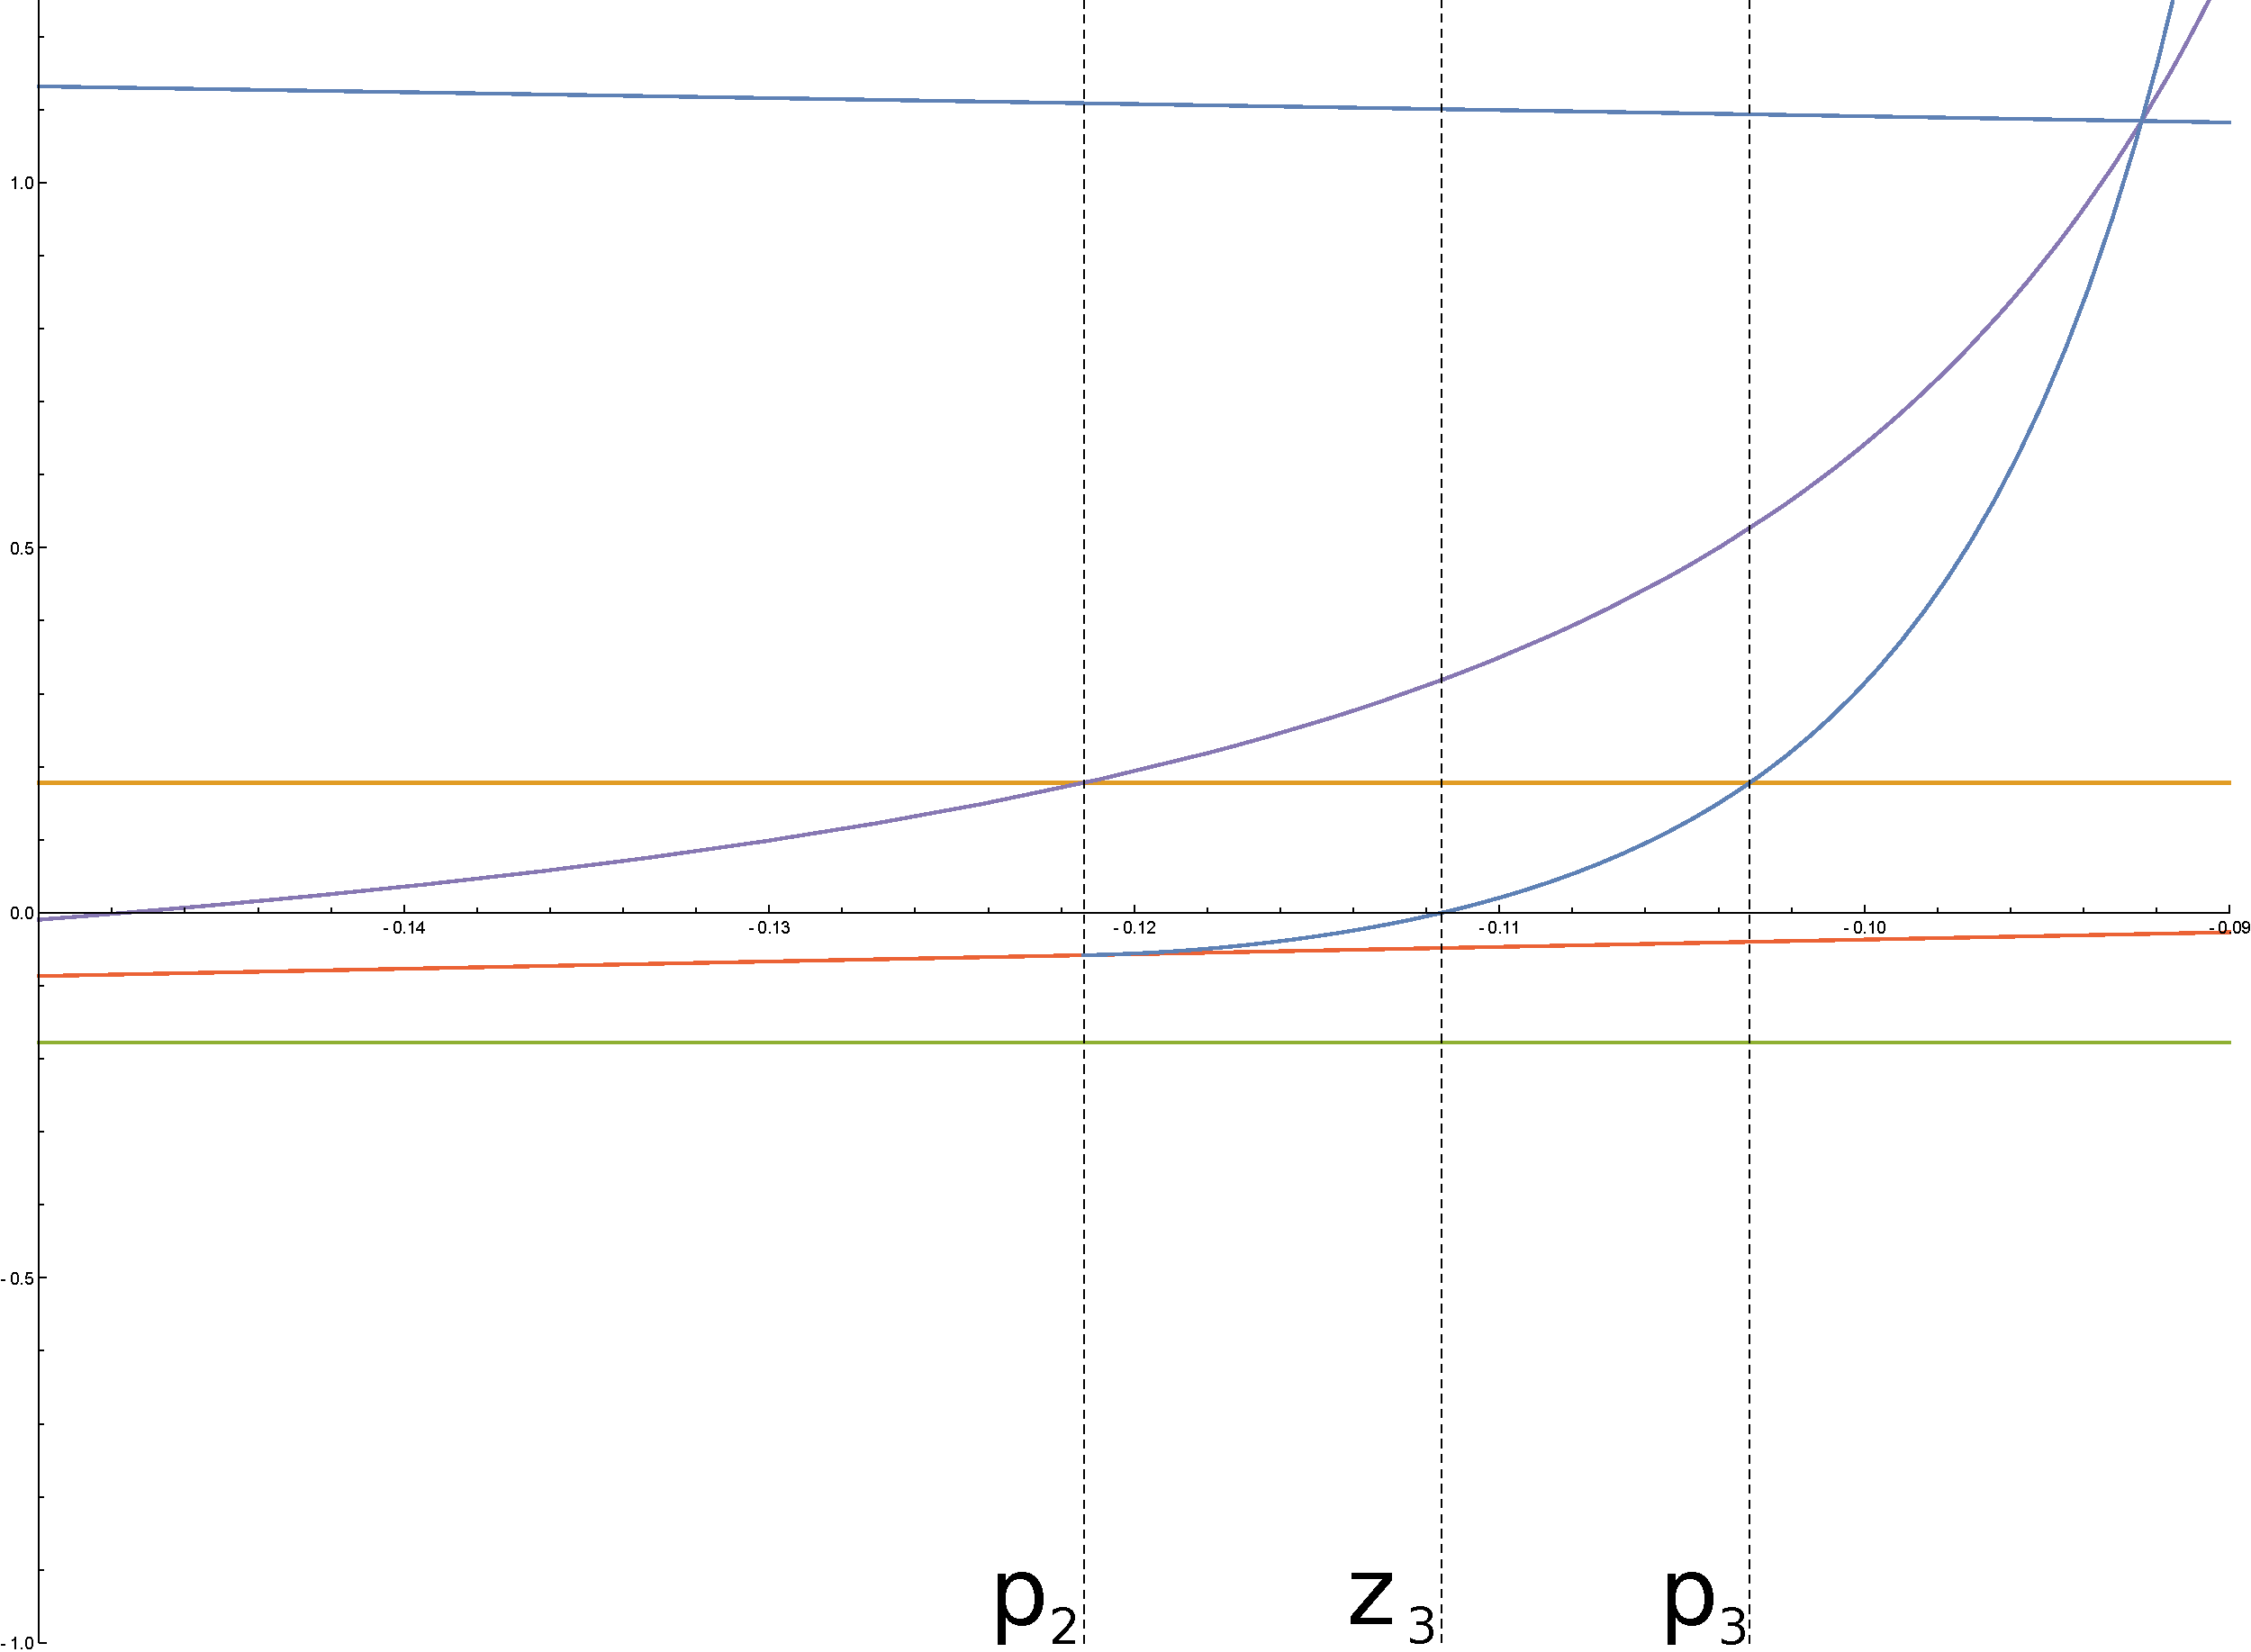
\includegraphics[width=\textwidth]{./img/cplot2H}
				\caption{$n=3$}
				\label{fig:cplot2H}
		\end{subfigure}
		\begin{subfigure}[b]{0.5\textwidth}
				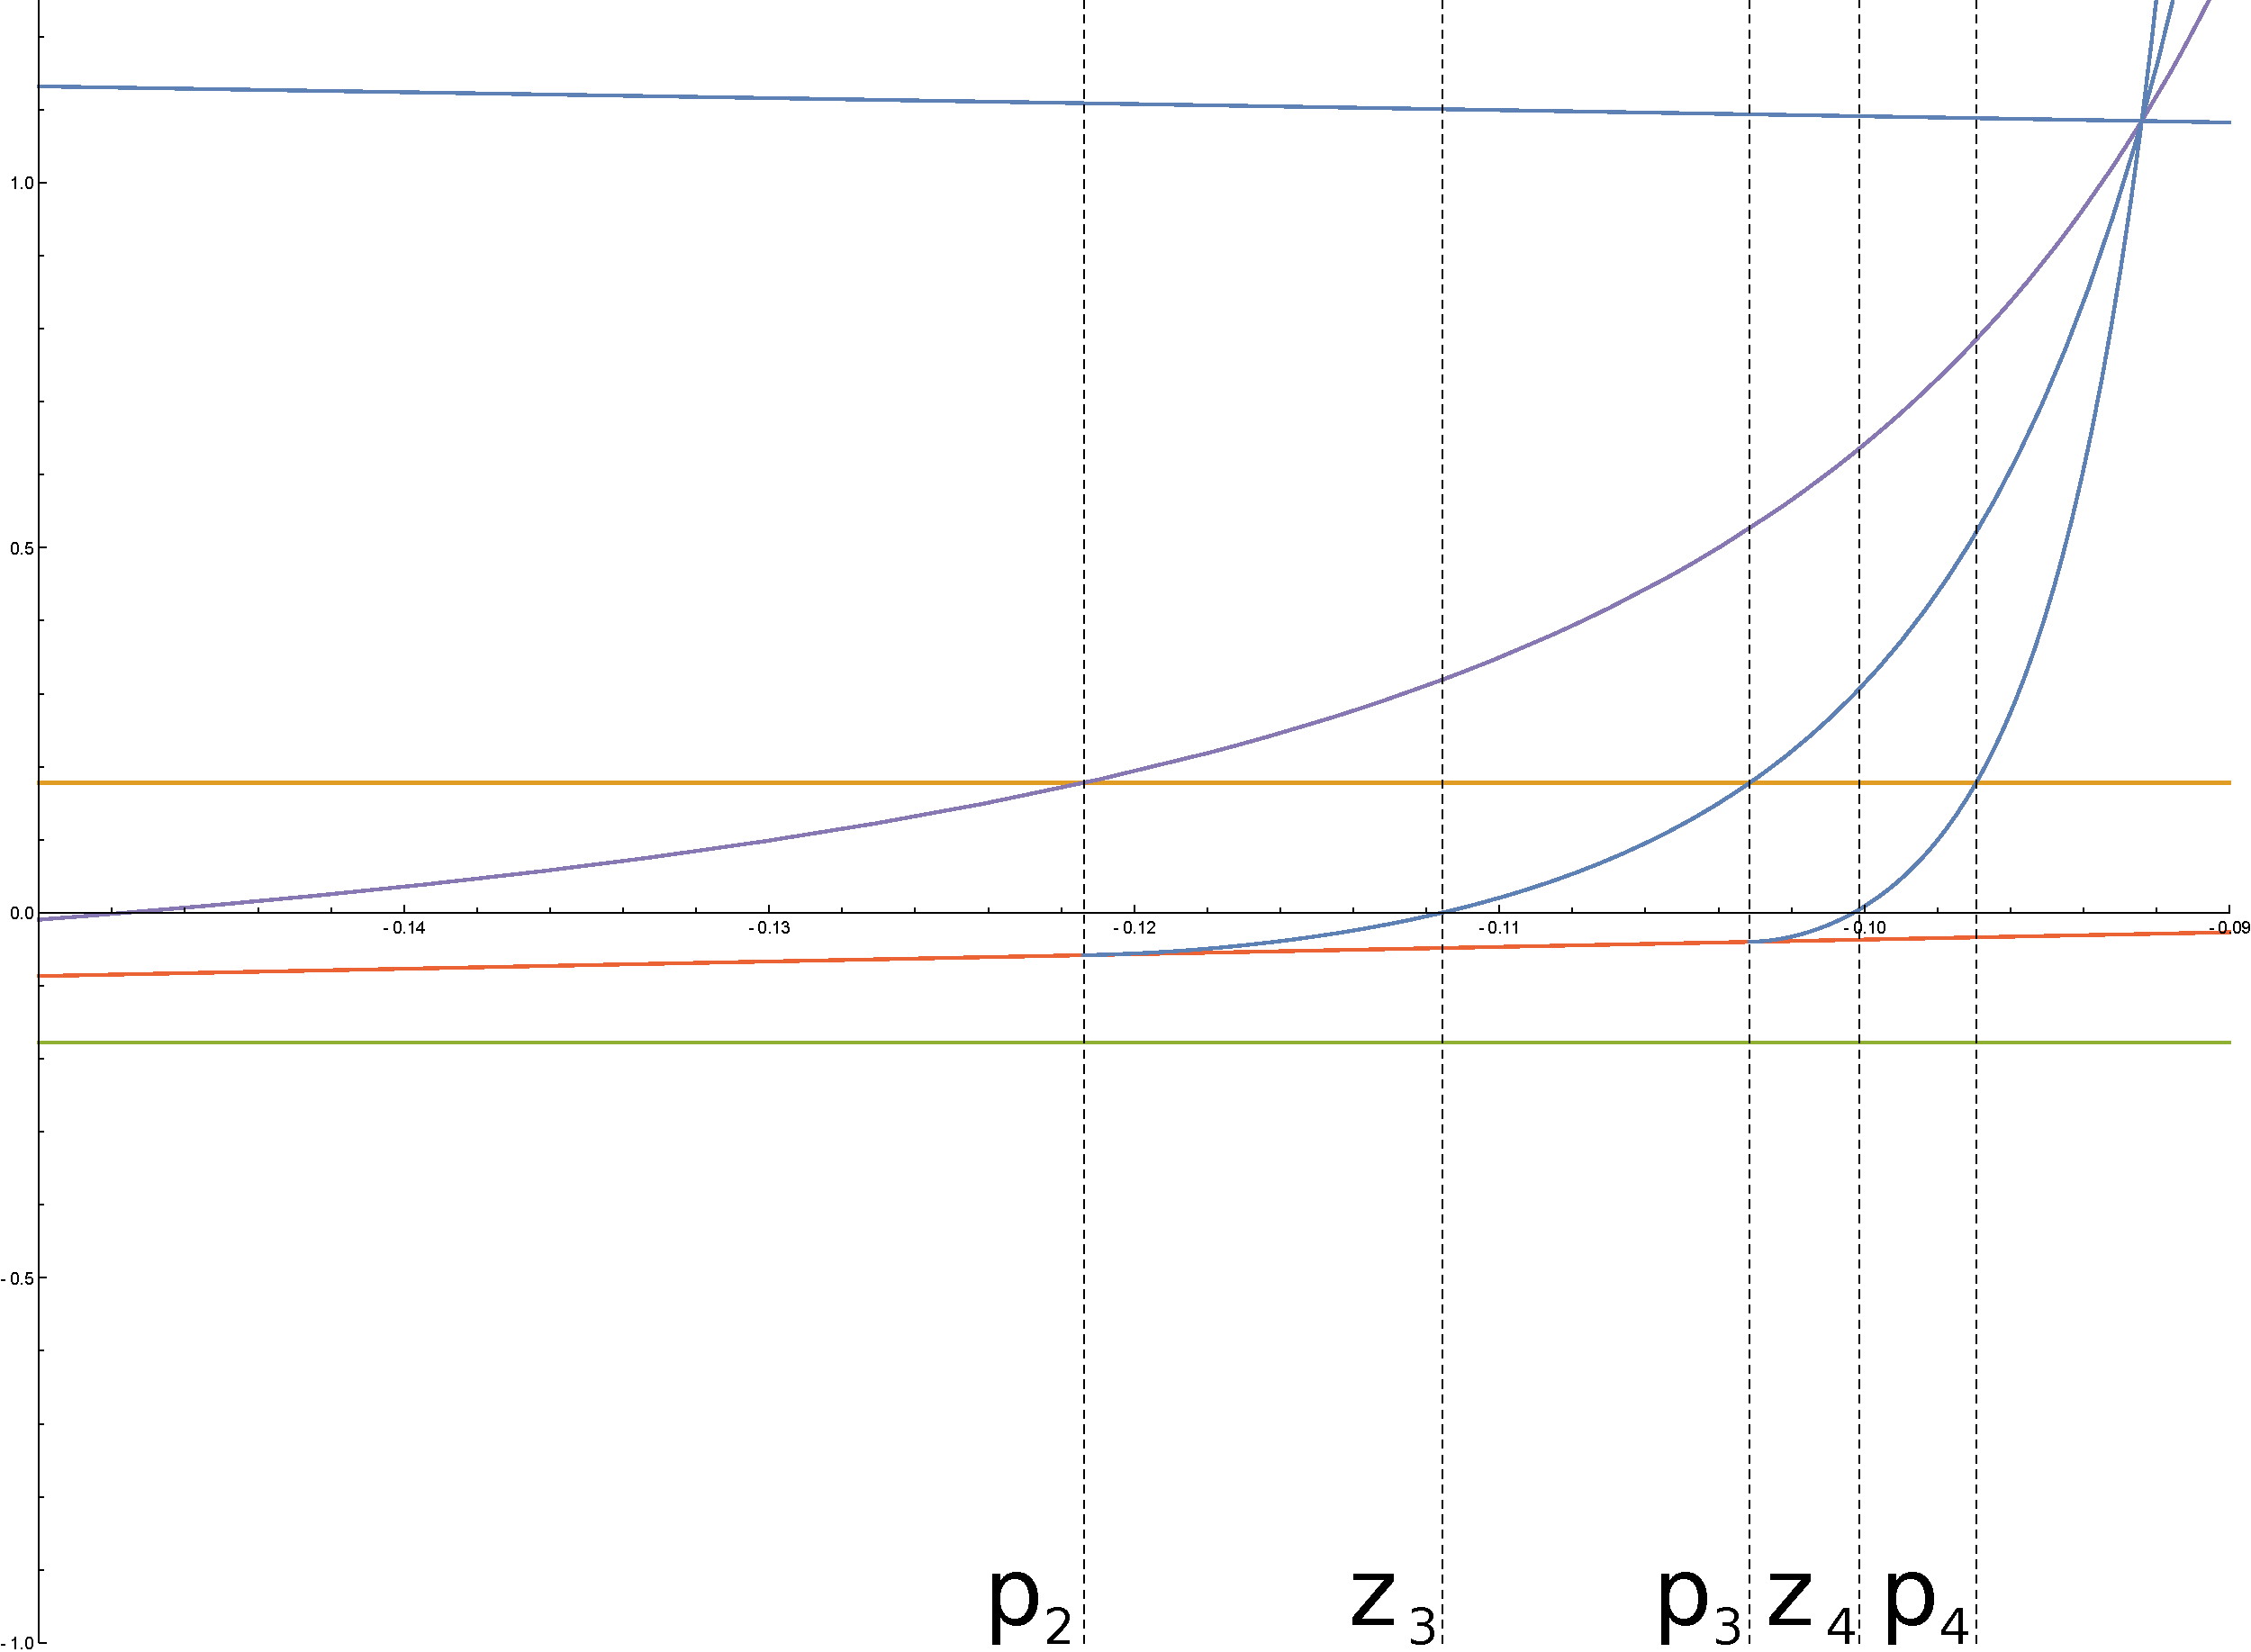
\includegraphics[width=\textwidth]{./img/cplot3H}
				\caption{$n=4$}
				\label{fig:cplot3H}
		\end{subfigure}%
		~ %add desired spacing between images, e. g. ~, \quad, \qquad, \hfill etc.
		  % (or a blank line to force the subfigure onto a new line)
		\begin{subfigure}[b]{0.5\textwidth}
				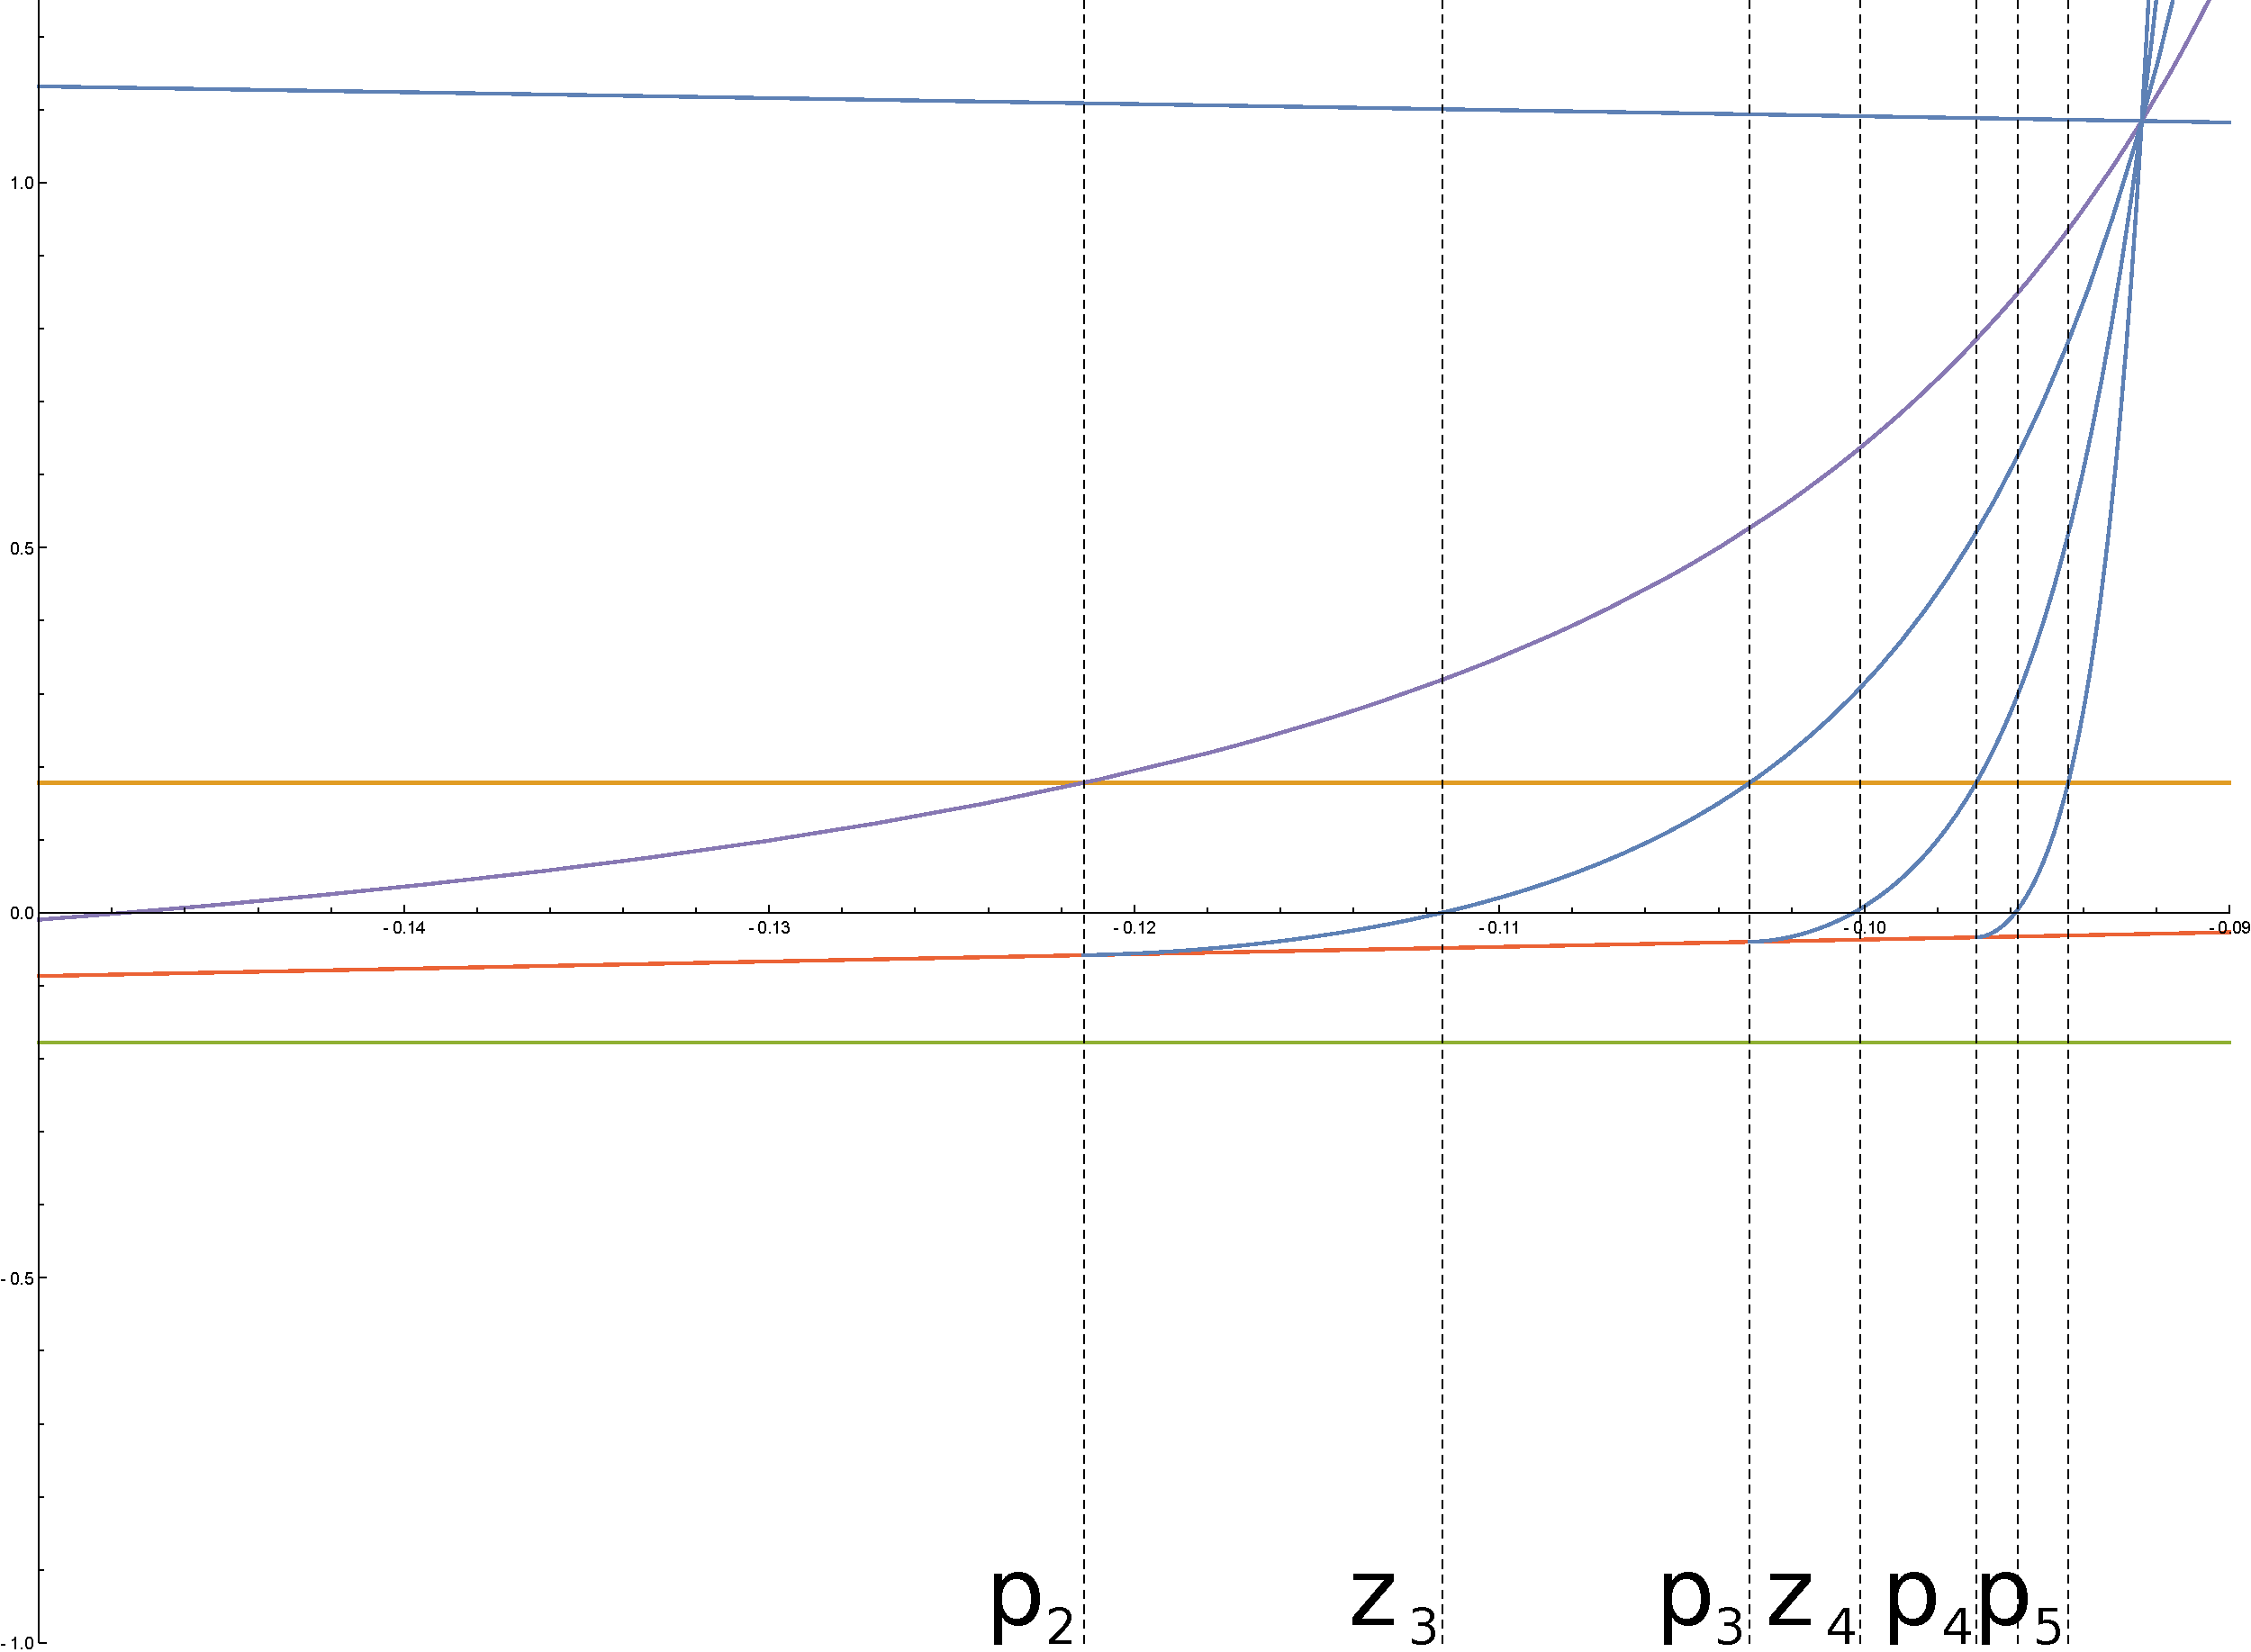
\includegraphics[width=\textwidth]{./img/cplot4H}
				\caption{$n=5$}
				\label{fig:cplot4H}
		\end{subfigure}
		\begin{subfigure}[b]{0.5\textwidth}
				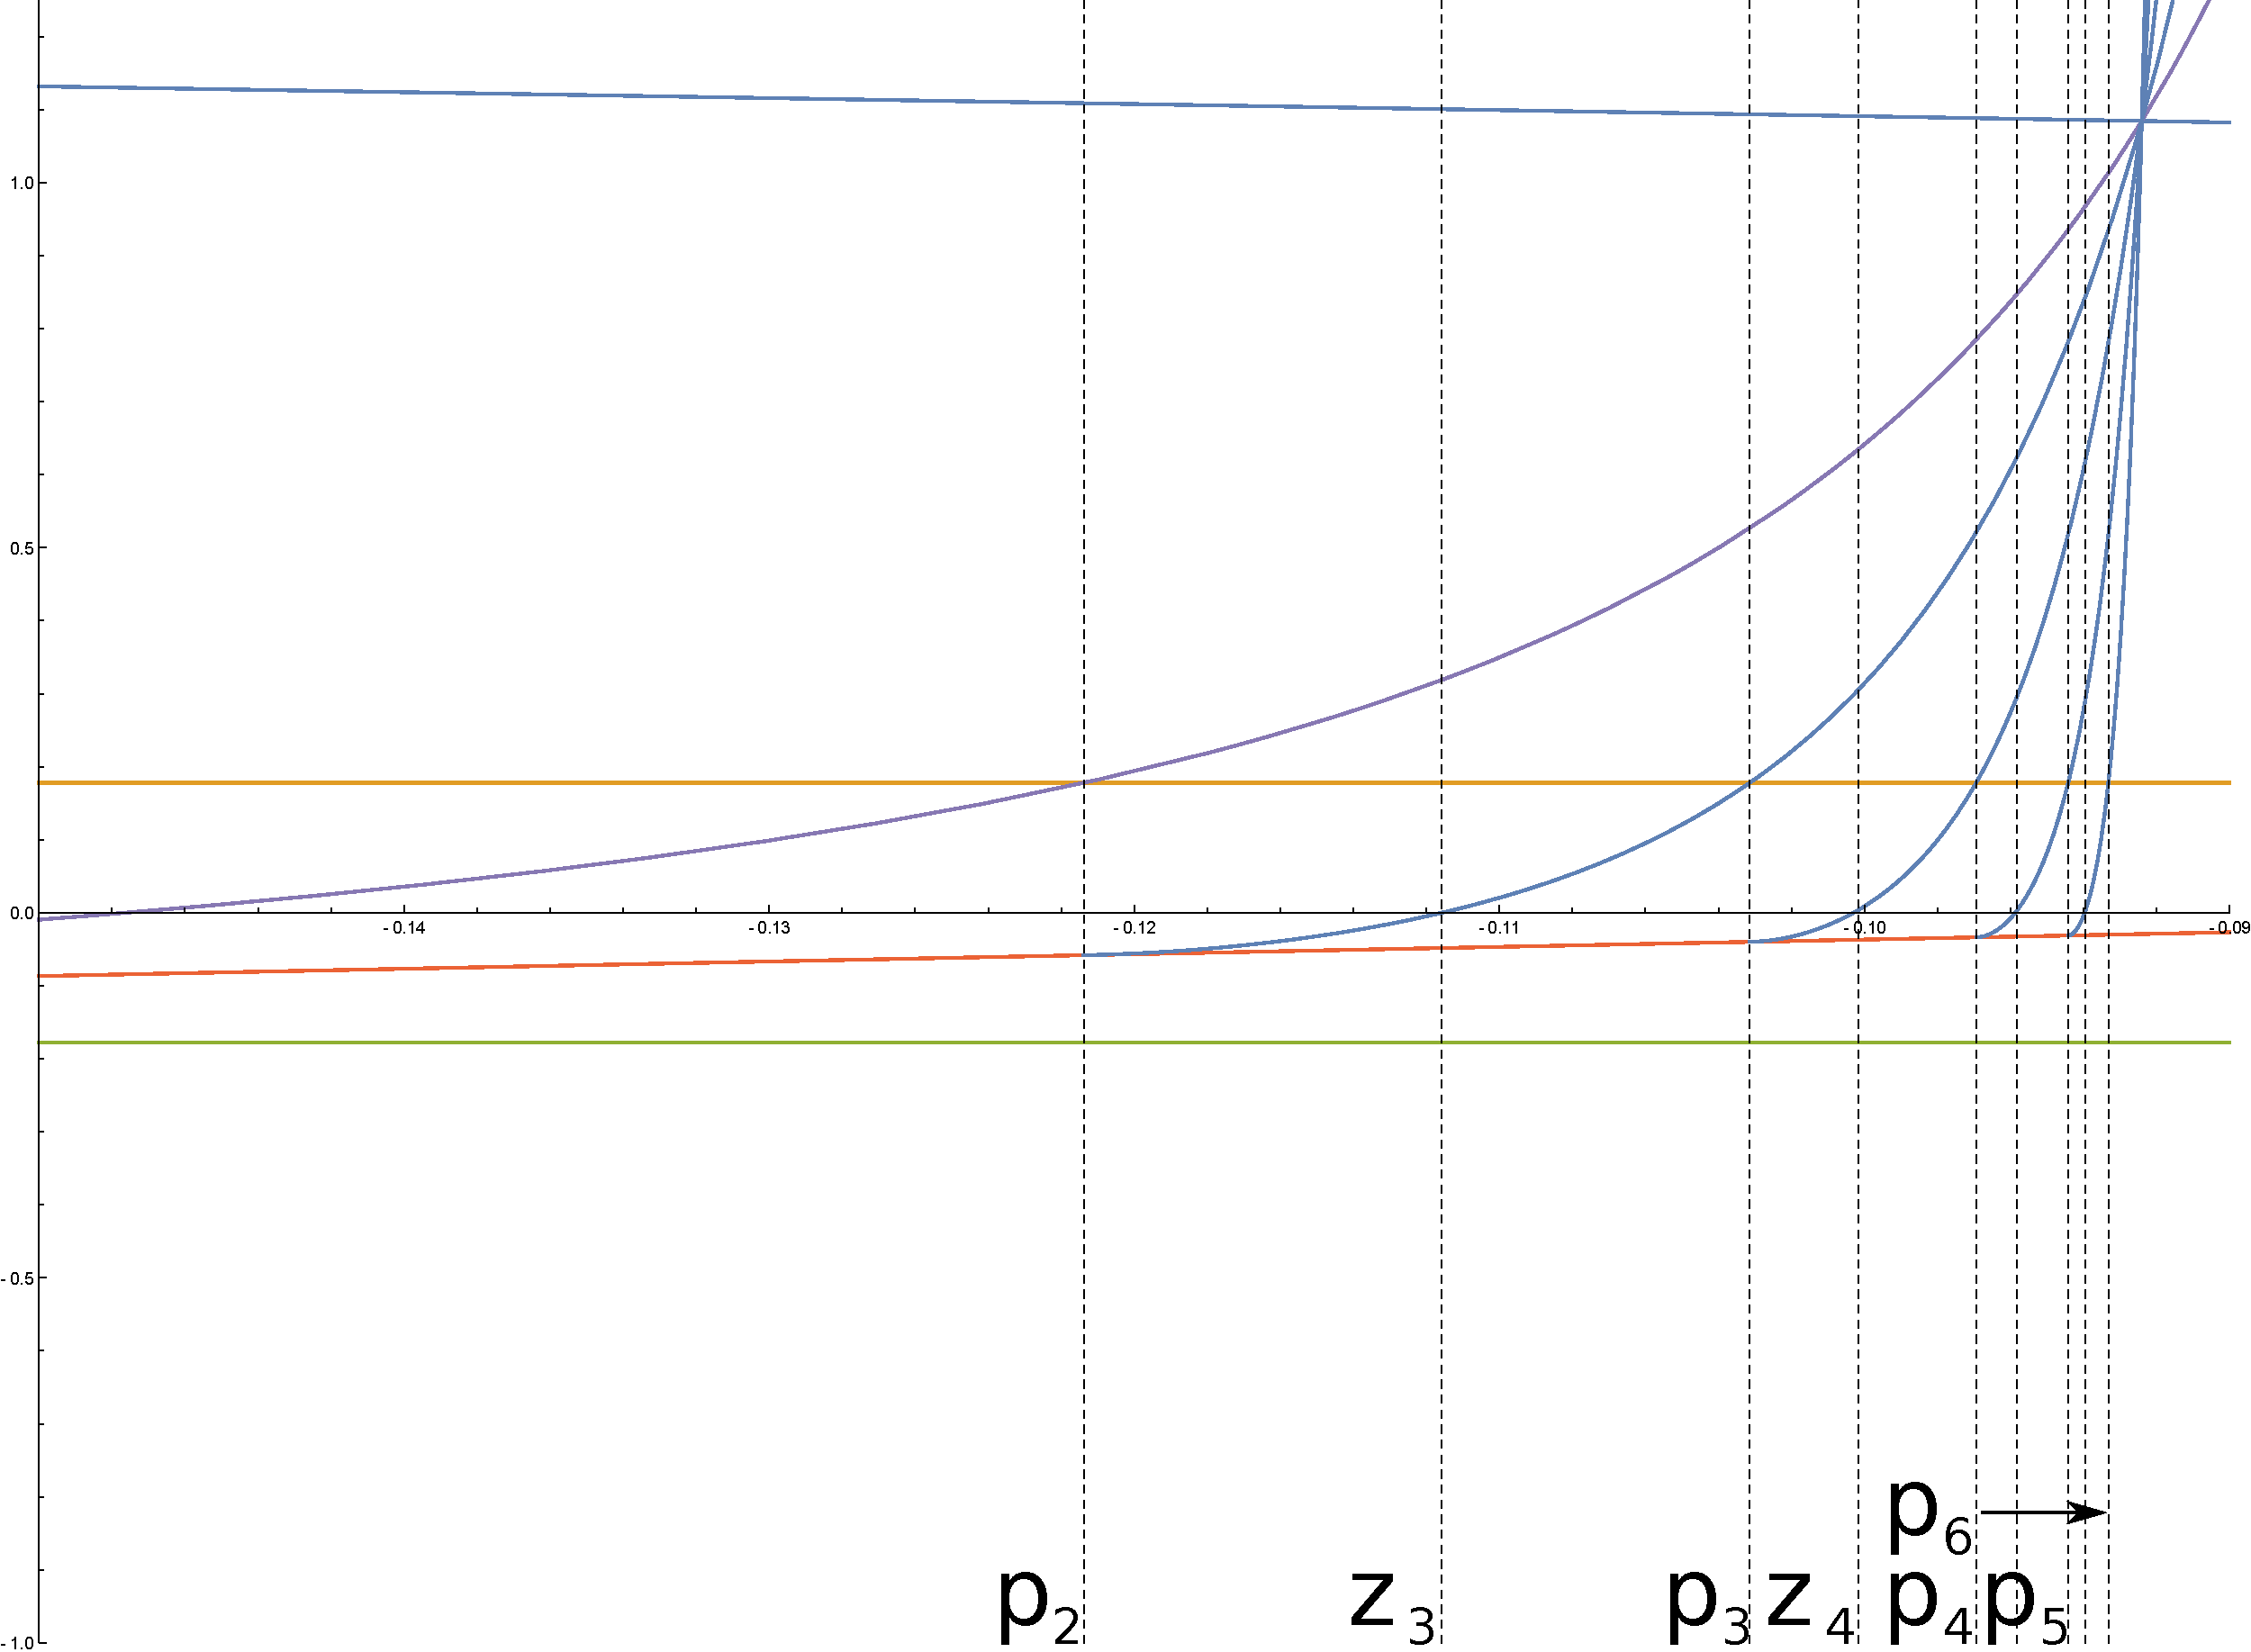
\includegraphics[width=\textwidth]{./img/cplot5H}
				\caption{$n=6$}
				\label{fig:cplot5H}
		\end{subfigure}%
		~ %add desired spacing between images, e. g. ~, \quad, \qquad, \hfill etc.
		  % (or a blank line to force the subfigure onto a new line)
		\begin{subfigure}[b]{0.5\textwidth}
				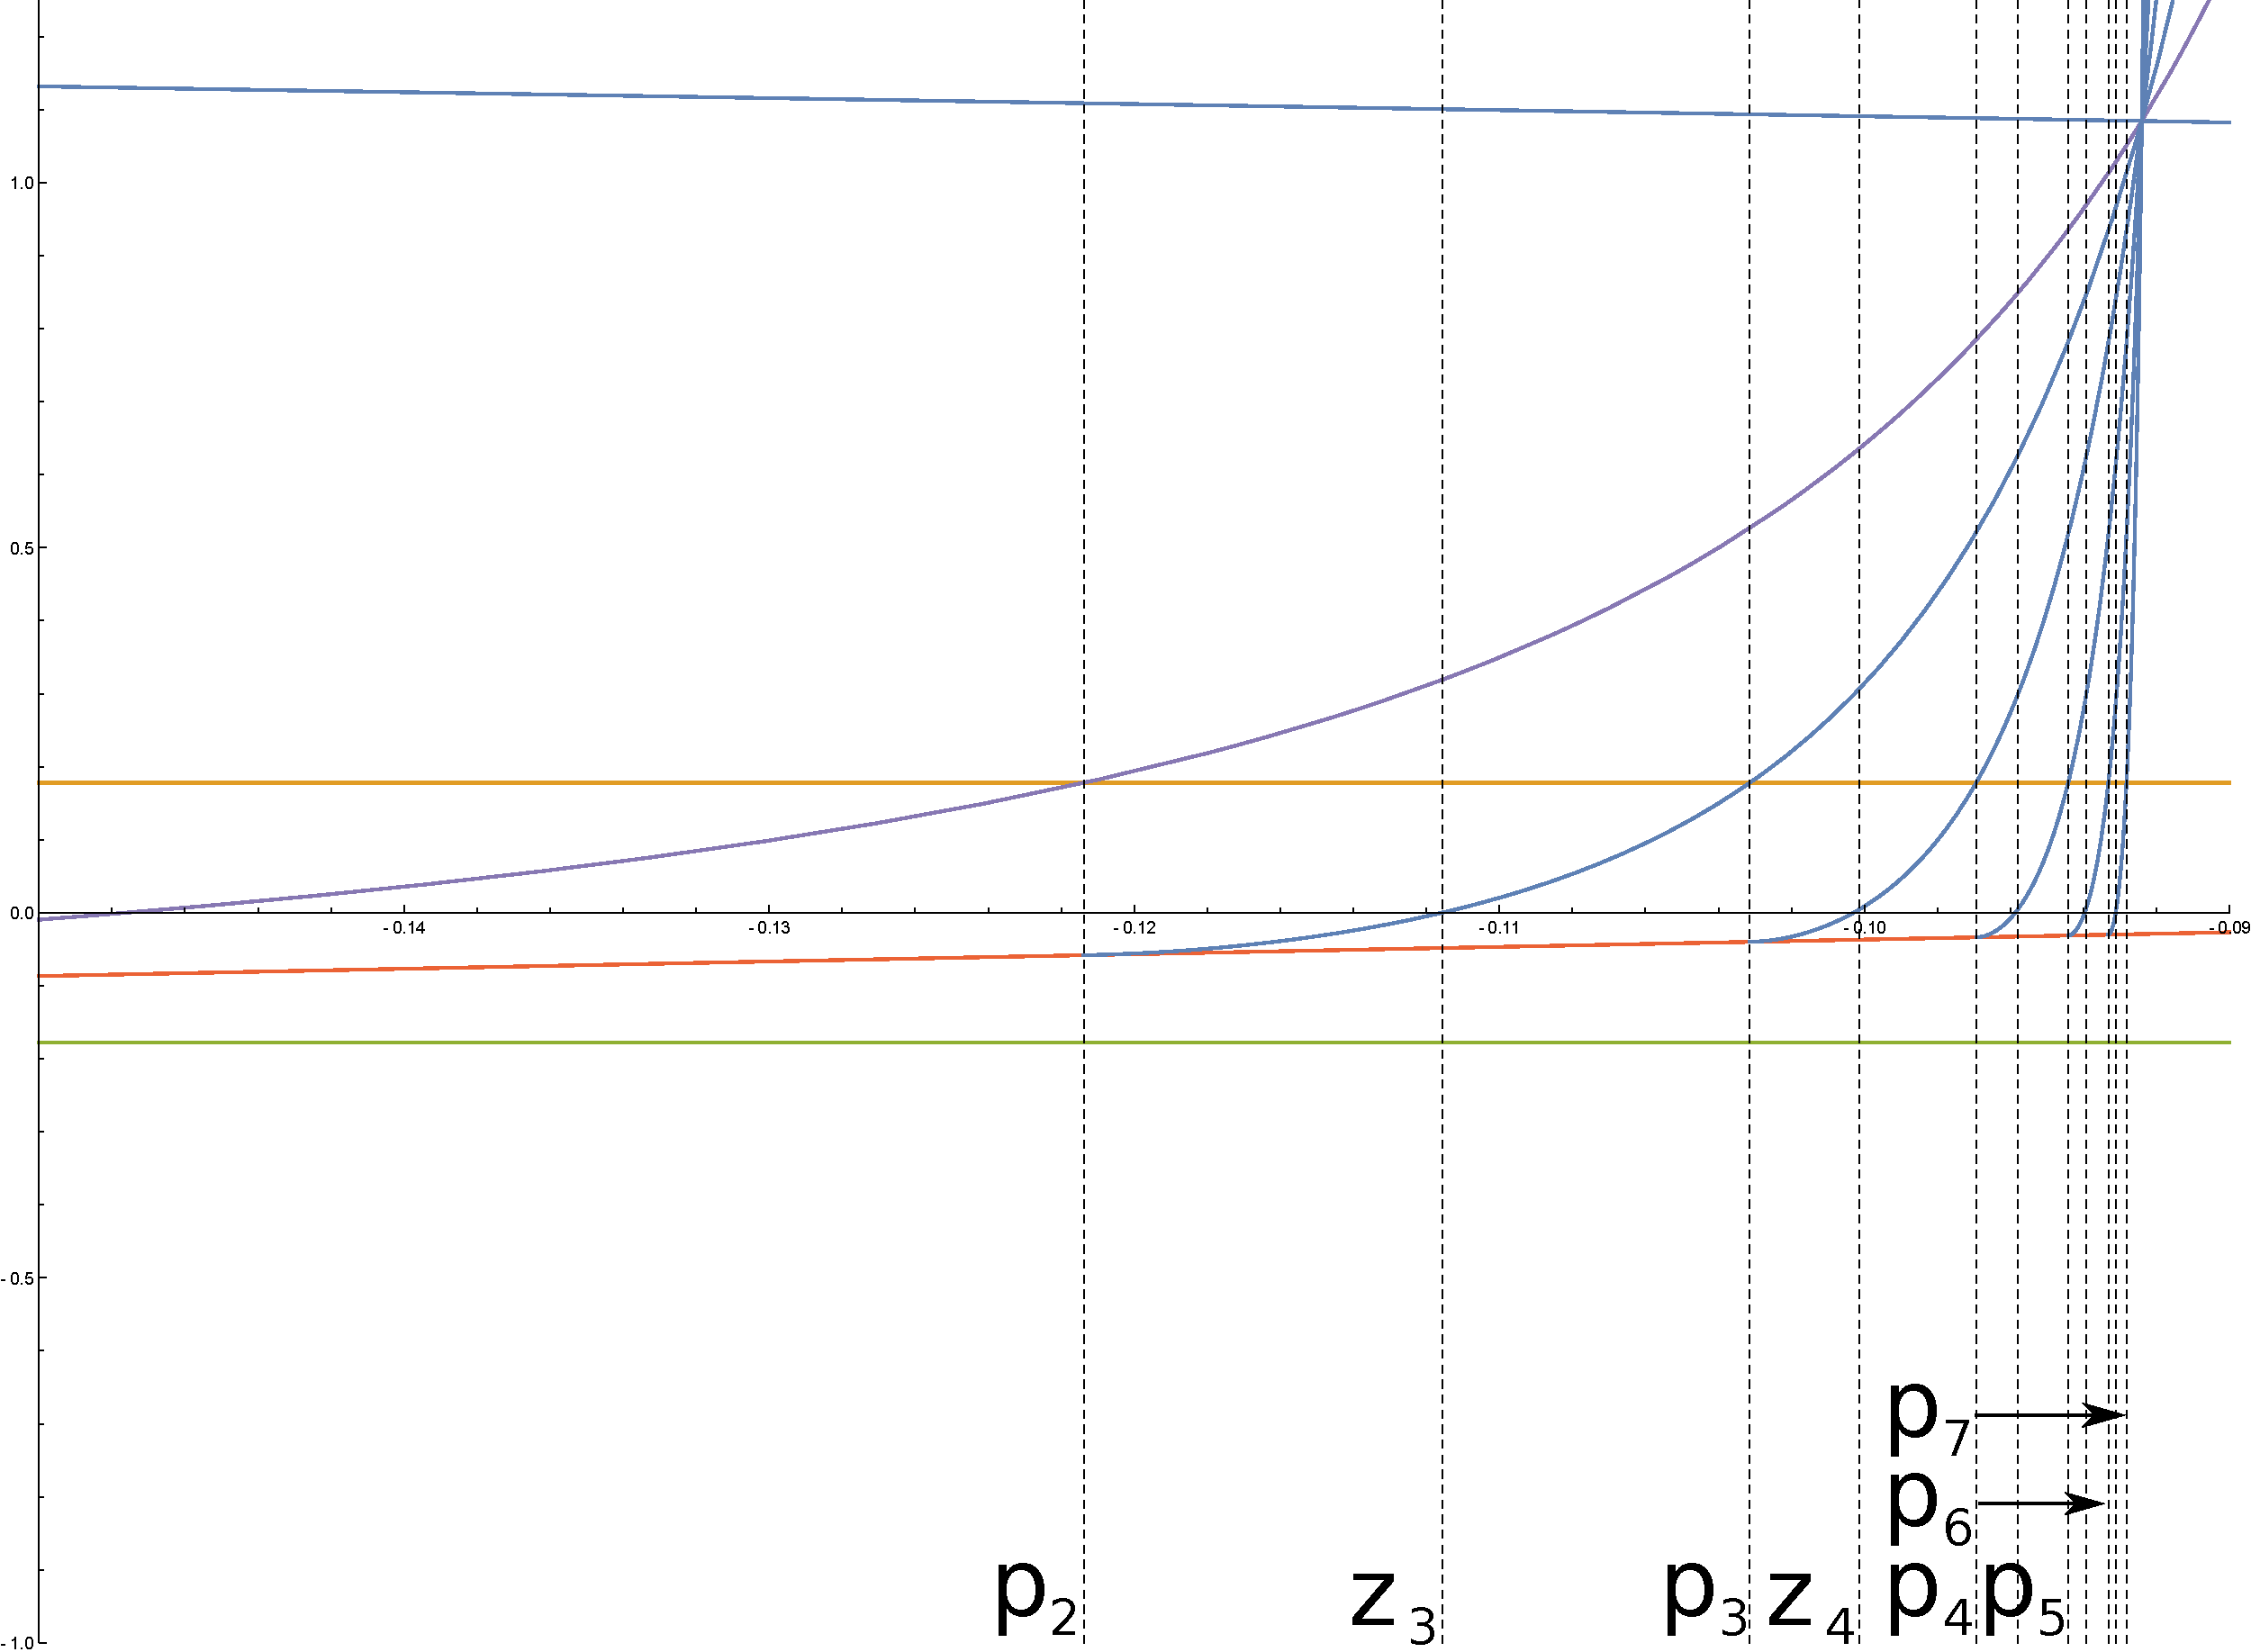
\includegraphics[width=\textwidth]{./img/cplot6H}
				\caption{$n=7$}
				\label{fig:cplot6H}
		\end{subfigure}
		~ %add desired spacing between images, e. g. ~, \quad, \qquad, \hfill etc.
		  % (or a blank line to force the subfigure onto a new line)
		% \caption{Plots of various iterates of $f_c (C)$ as a function of $c$ depicting the accumulation of prezero and periodic parameter values as we approach $h_2^{CrP_c}$ from the left. Note that for $n > 4$ the $z_n$ values are marked but not labeled}\label{fig:iterh}
\end{figure}
\end{frame}
\begin{frame}{An Infinite Hierarchy}
\begin{proposition}

		Suppose we have two distinct parameter values $z_{n_1}^{C\alpha0}, z_{n_2}^{C\beta0} \in (\pl, \pr)$ where $\alpha$ and $\beta$ are coding sequences such that $\alpha_i \neq \beta_i$ for at least one $i$. Then there must be at least two other prezero parameter values $z_{n_3}^{\gamma}$ and $z_{n_4}^{\delta}$ on the interval $\inte{z_{n_1}^{C\alpha 0}}{z_{n_2}^{C\beta 0}}$ such that $\gamma_i \neq \delta_i$ for at least one $i$.

\end{proposition}
\end{frame}

\begin{frame}{Plot of Critical Point}
	\begin{figure}
		\centering
		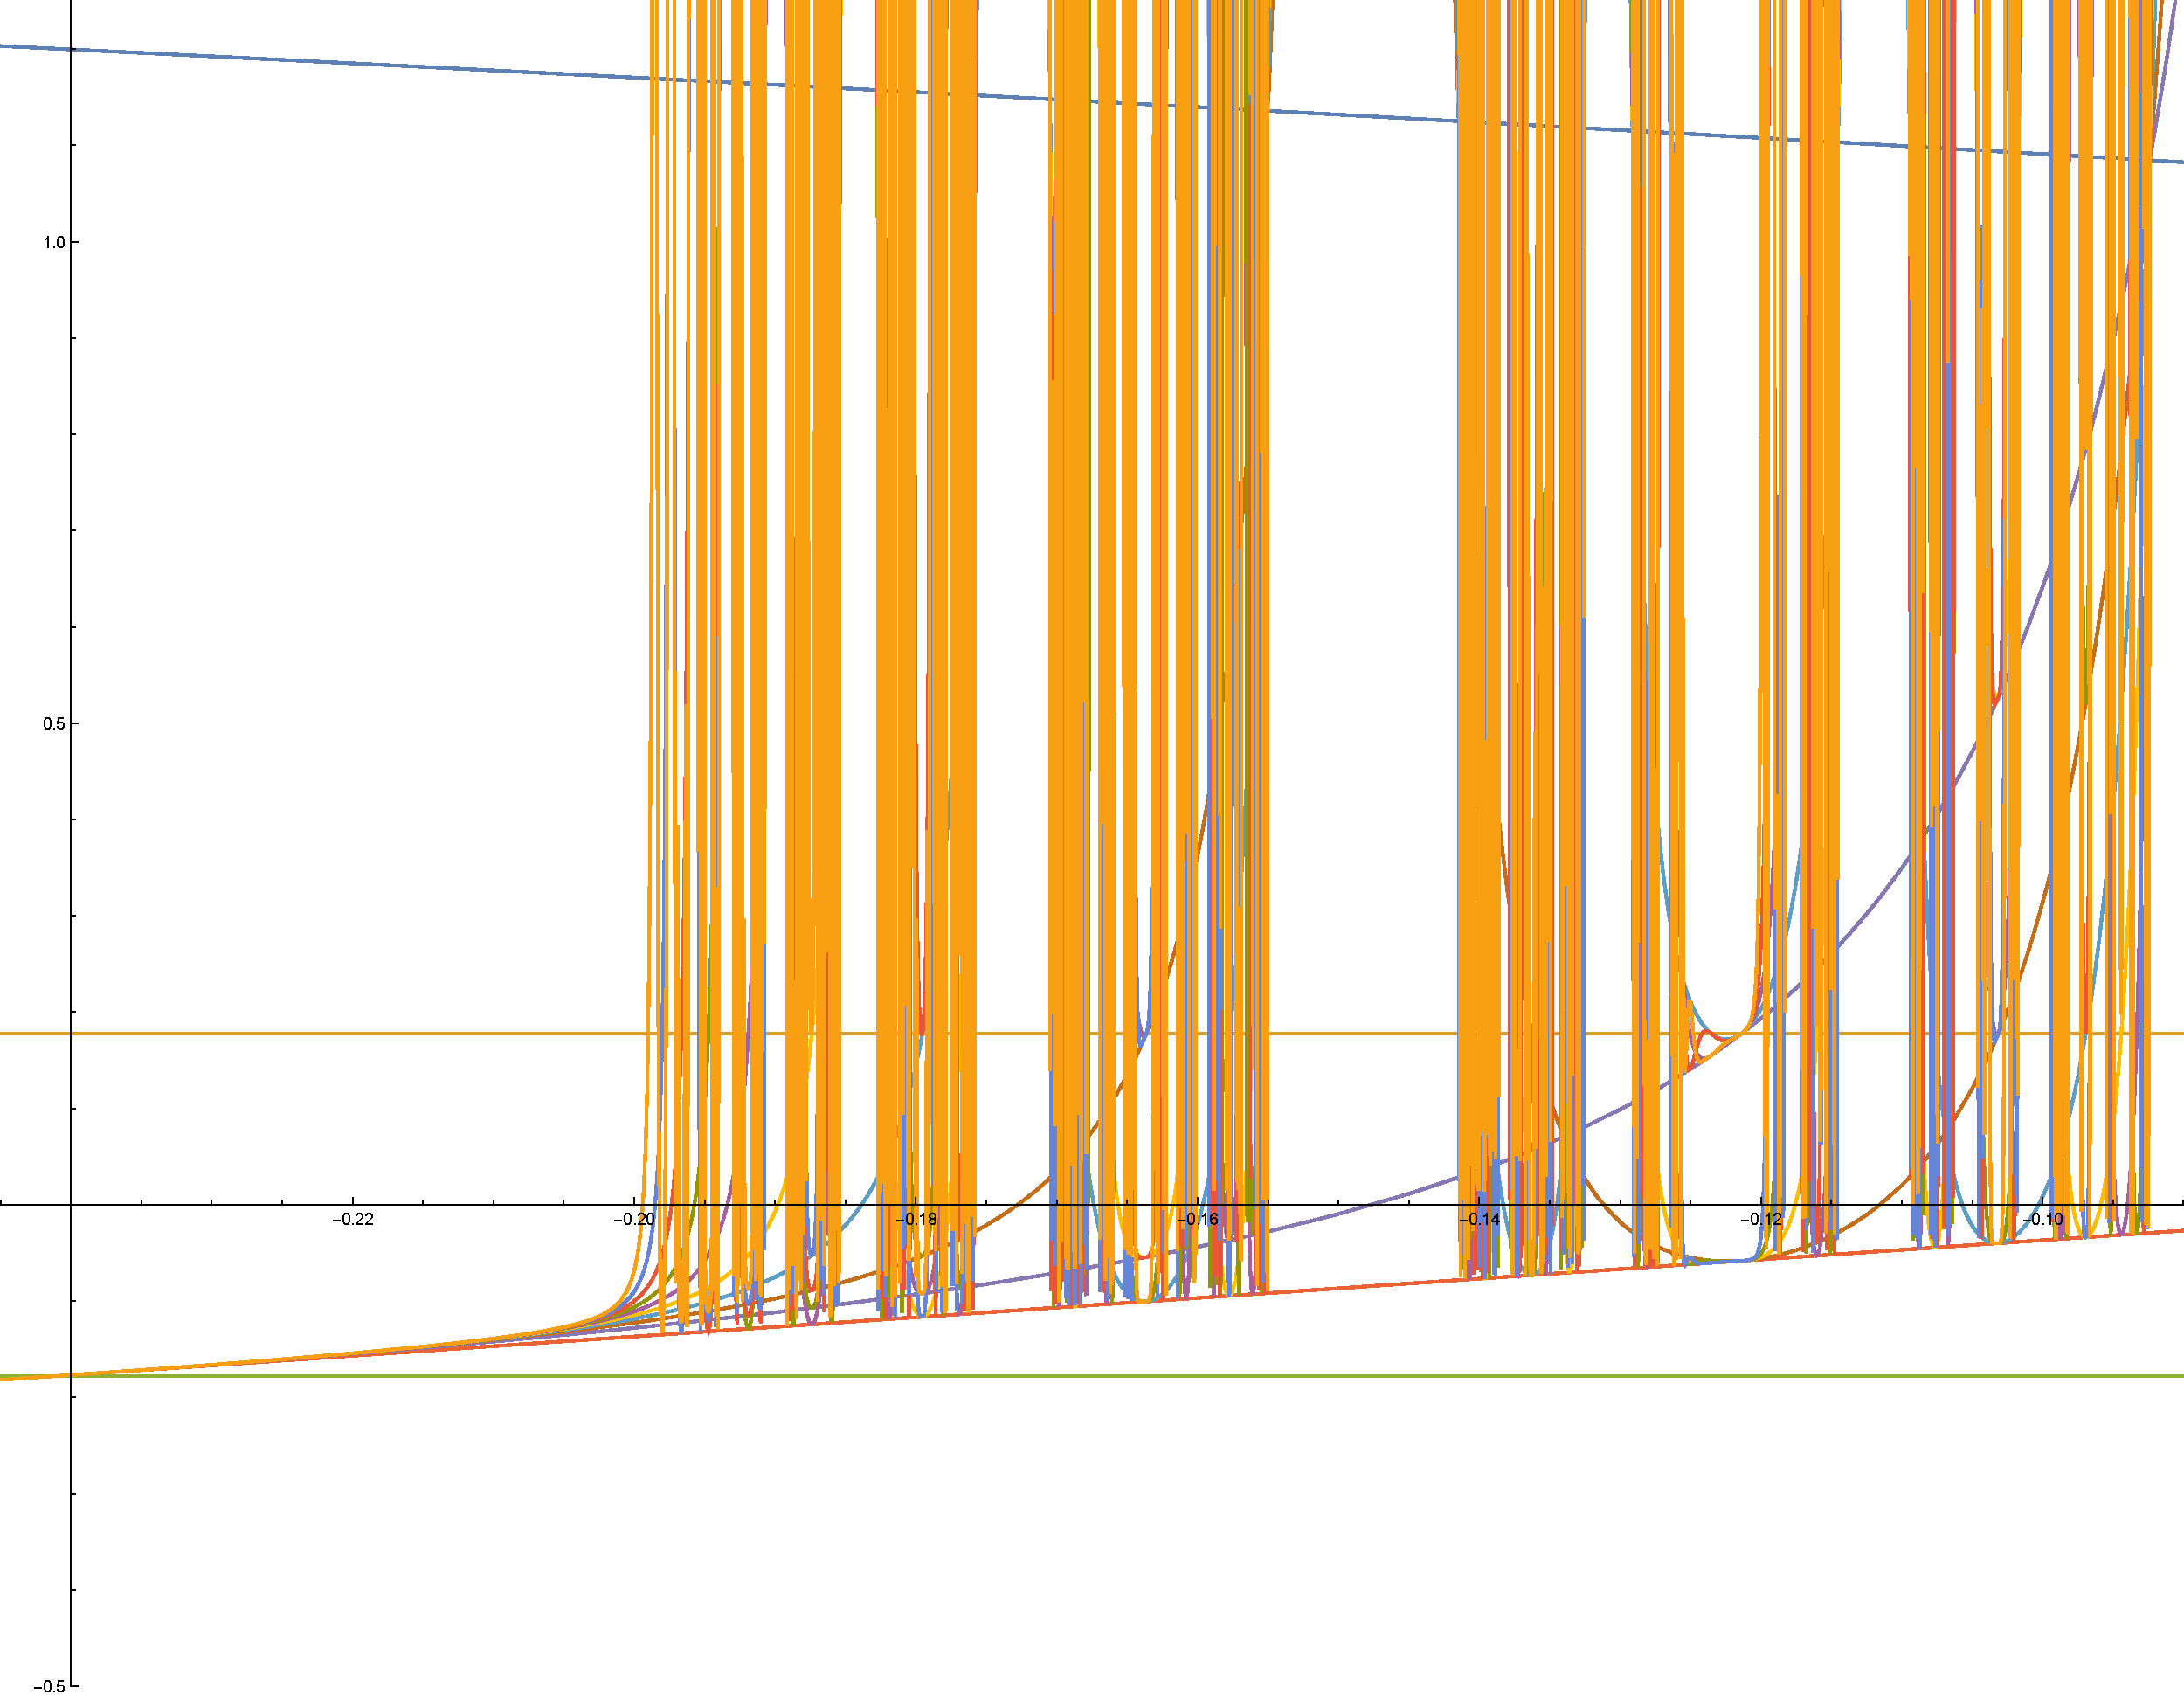
\includegraphics[width=.8\textwidth]{./img/10it}
		\caption{\footnotesize Plot of first 10 iterates of $C$ for $c \in (-.245,-0.09) \approx (\pl,\pr)$}
	\end{figure}
\end{frame}

\begin{frame}{Back to the Plane}
	\begin{figure}[h]
	\centering
	\begin{subfigure}[b]{0.49\textwidth}
			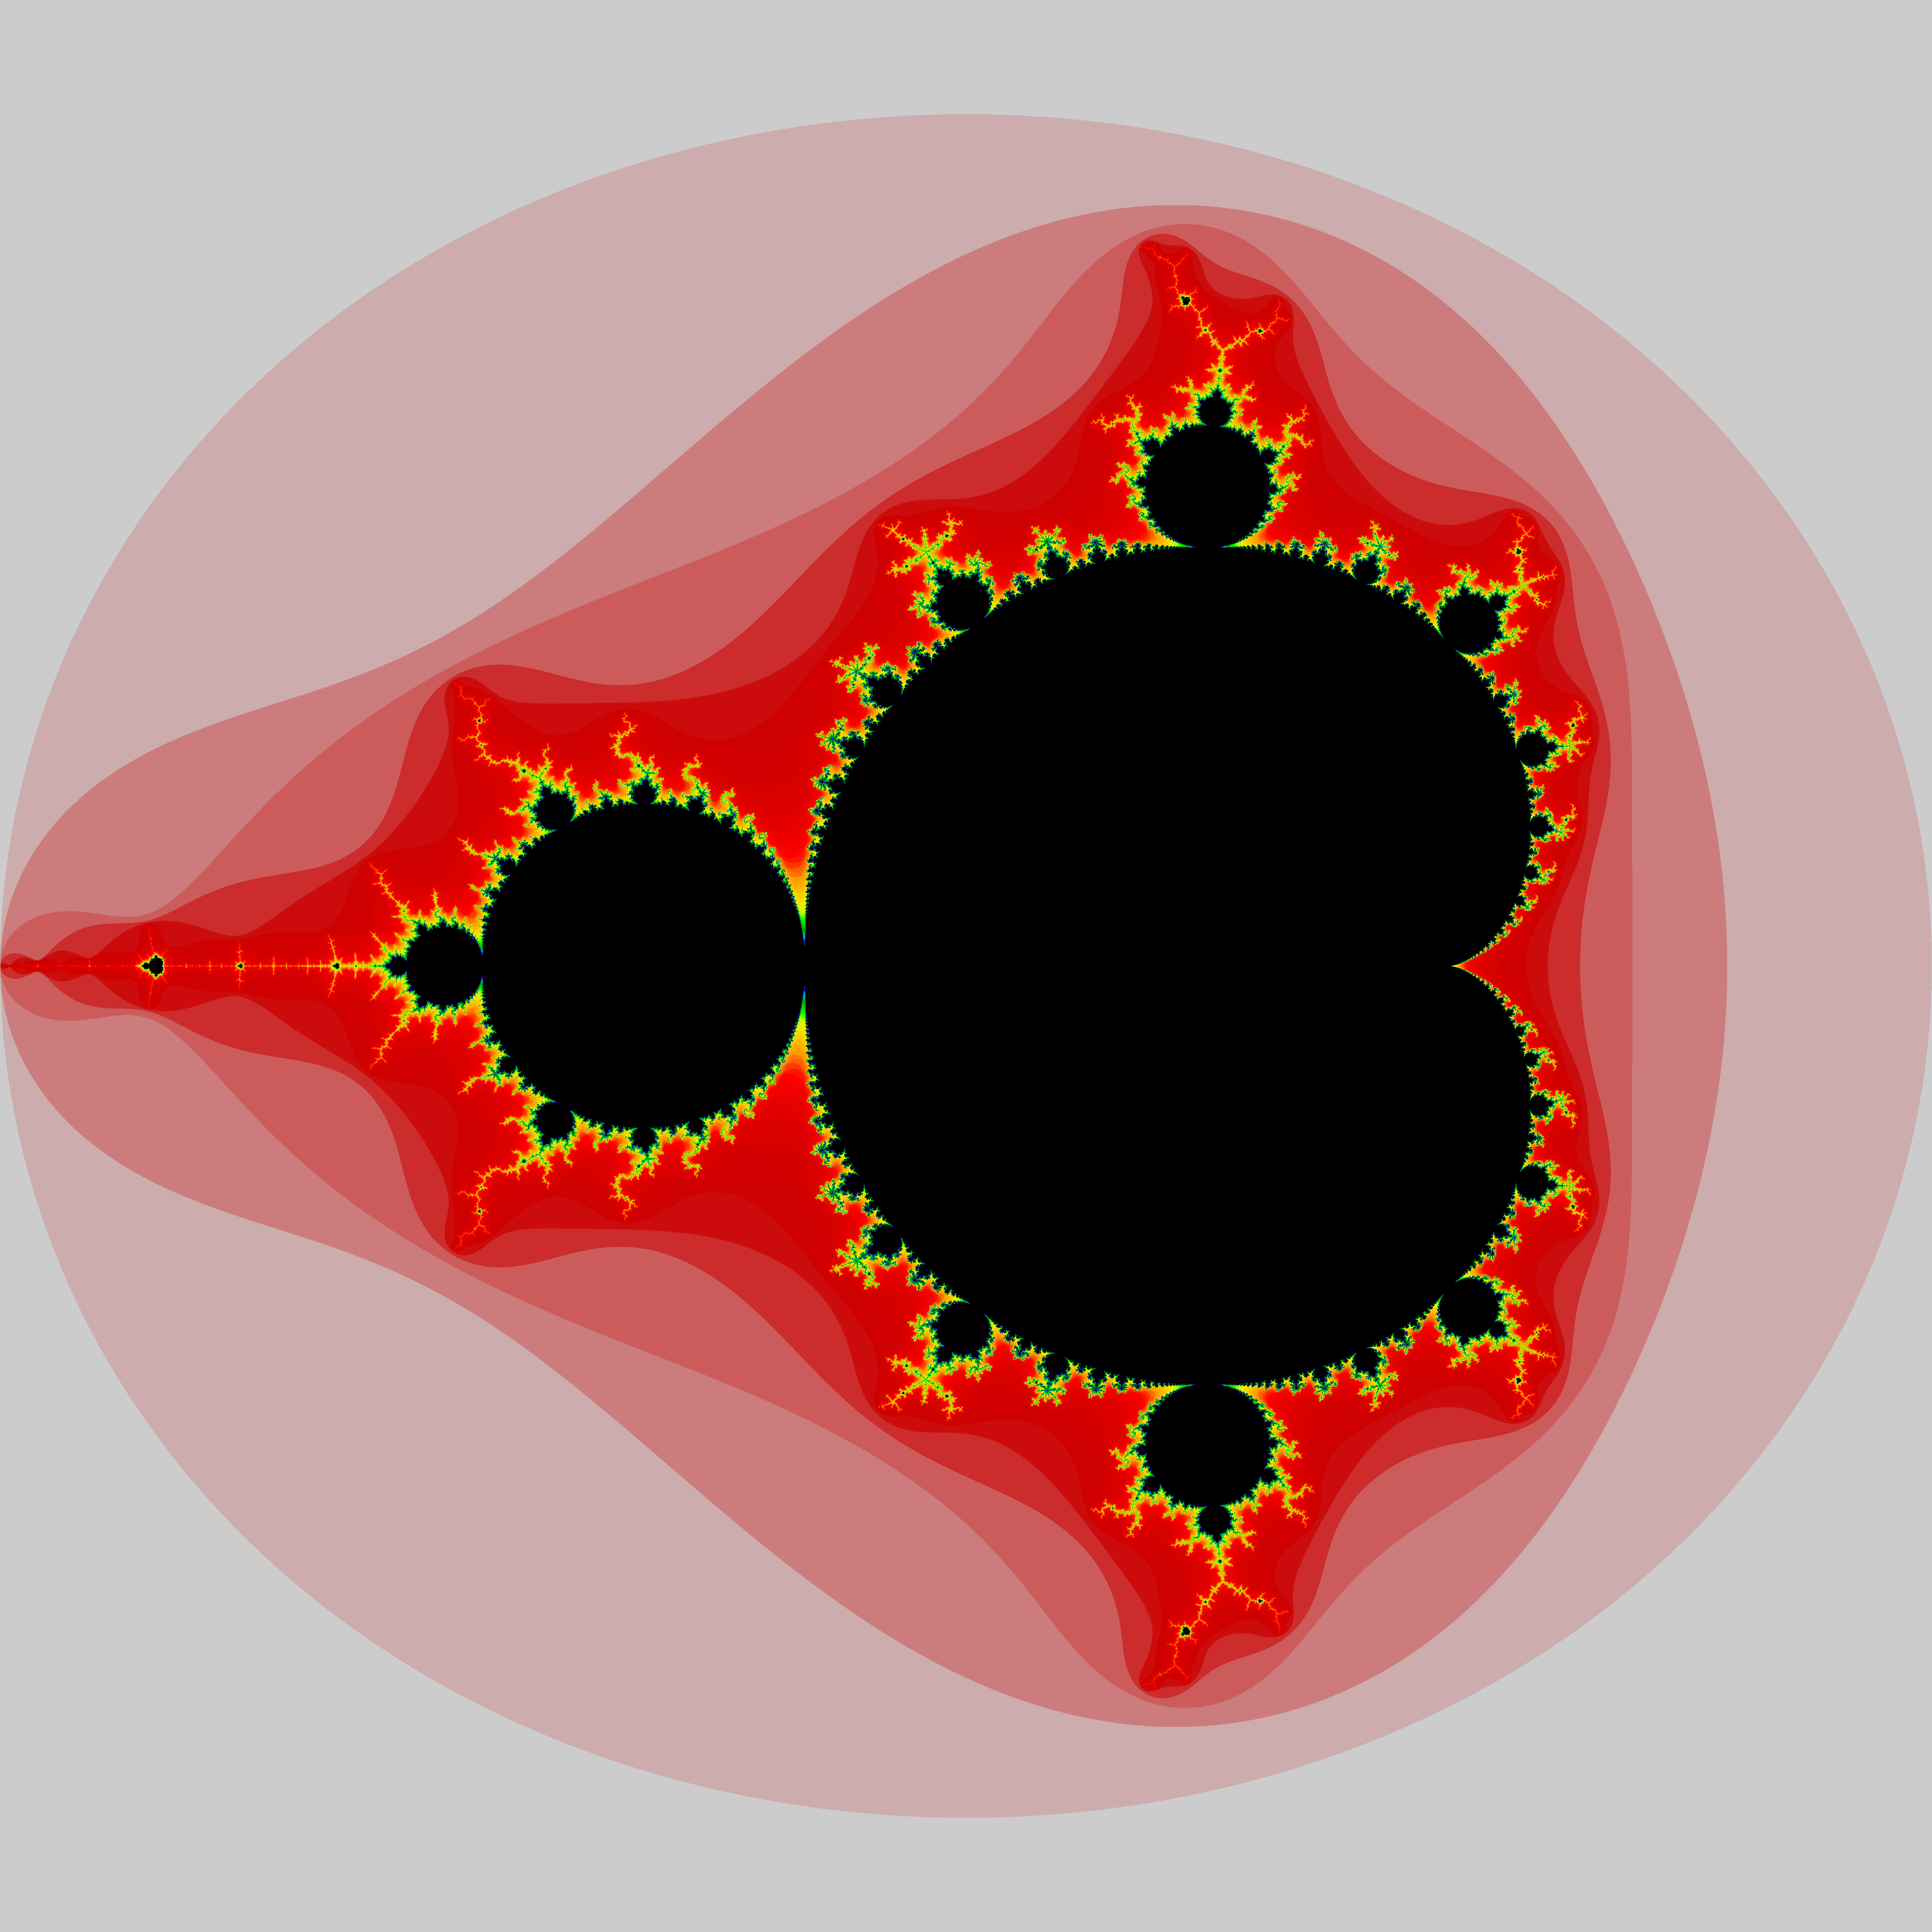
\includegraphics[width=\textwidth]{./img/b000}
			\caption{Parameter Space Escape Picture for $z^2 + c$}
	\end{subfigure}%
	\begin{subfigure}[b]{0.49\textwidth}
			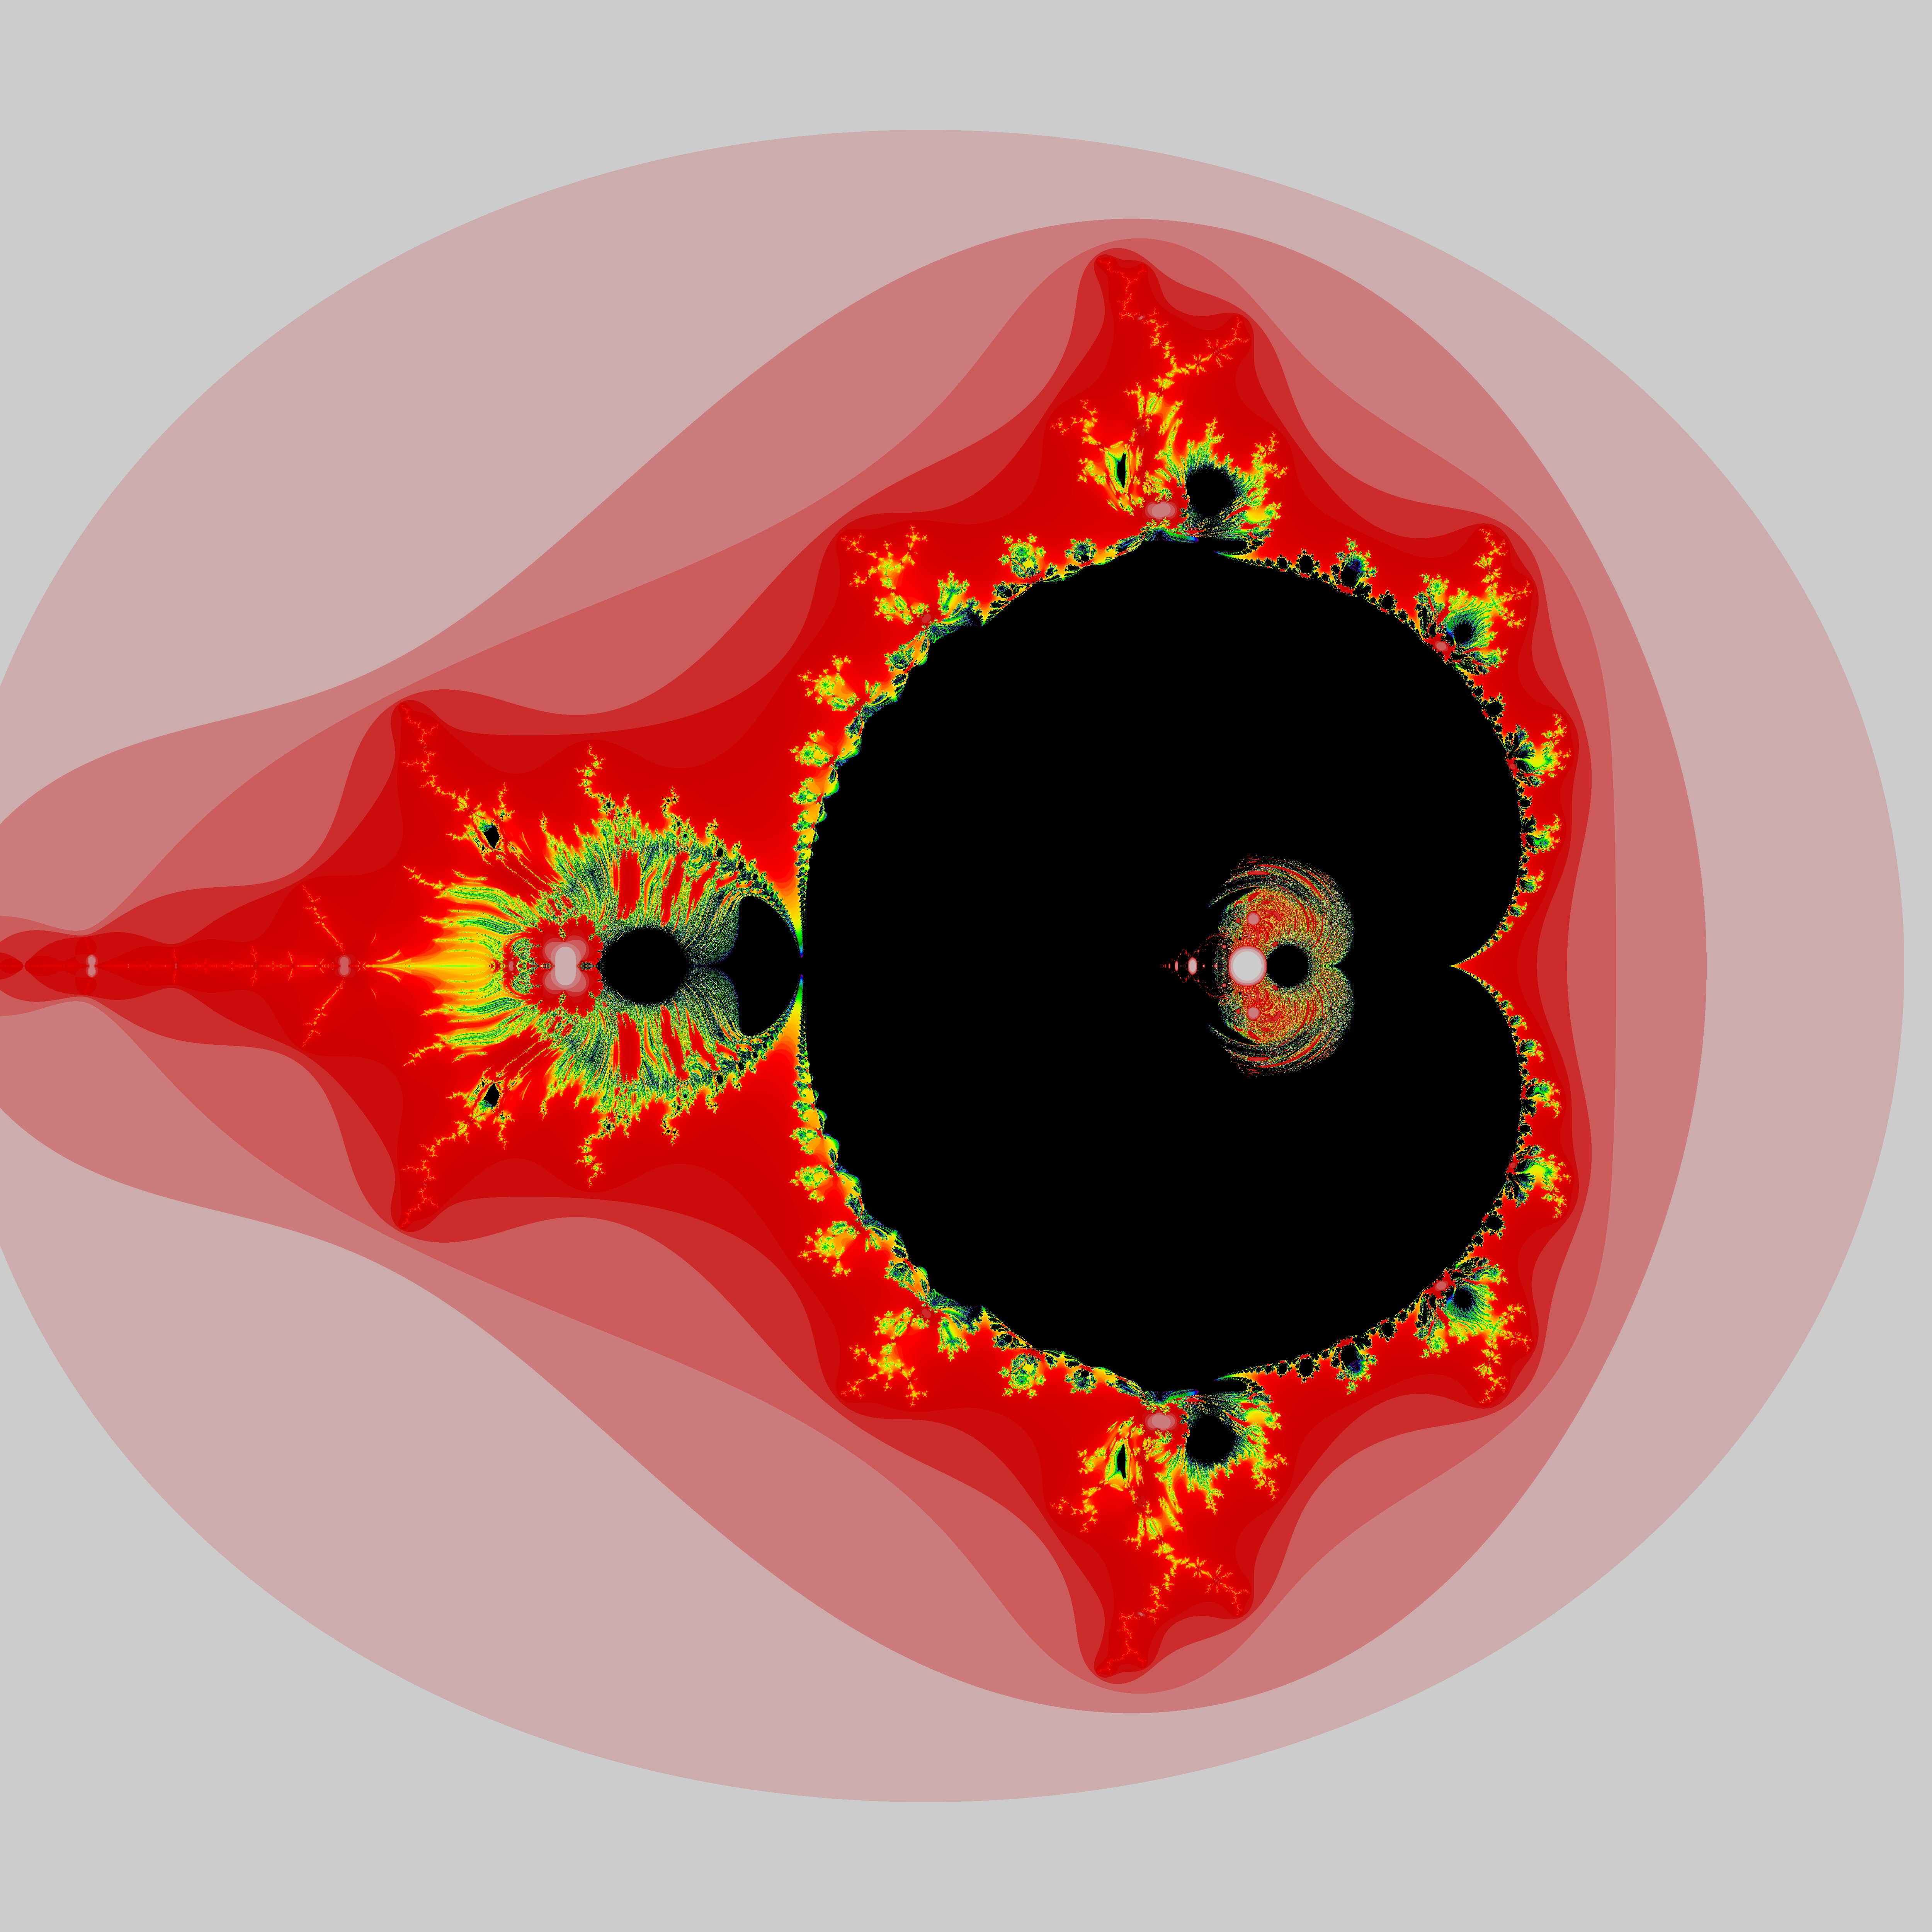
\includegraphics[width=\textwidth]{./img/b001}
			\caption{Parameter Space Escape Picture for $z^2 + c + \frac{.001}{\overline{z}^2}$}
	\end{subfigure}
	%\caption{Orbit diagrams of the original and perturbed systems}\label{fig:perdub}
\end{figure}
\end{frame}

% \begin{frame}
% \begin{rawhtml}
% <p><script src="http://www.wolfram.com/cdf-player/plugin/v1.0/cdfplugin.js"
% type="text/javascript"></script><script type="text/javascript">// <![CDATA[
% var cdf = new cdf_plugin ();
% cdf.addCDFObject ("source", "source.cdf",840,670);
% // ]]></script>

% <img id="source" src="screen_shot.png" 
%  alt="screen_shot" />
% \end{rawhtml}
% \end{frame}
\section{References}
\begin{frame}
\frametitle{Bibliography}
\nocite{*}
\bibliographystyle{plain}
\bibliography{sources}
\end{frame}

\end{document}